%
% Master thesis template for Ghent University (2018)
%
%
%  !!!!!!!!!!!!!!!!!!!!!!!!!!!!!!!!!!!!!!!!!!!!!!!!!!!!!!!!!!!!
%  !!  MAKE SURE TO SET lualatex OR xelatex AS LATEX ENGINE  !!
%  !!!!!!!!!!!!!!!!!!!!!!!!!!!!!!!!!!!!!!!!!!!!!!!!!!!!!!!!!!!!
%  !! For overleaf:                                          !!
%  !!     1. click gear icon in top right                    !!
%  !!     2. select `lualatex` in "latex engine"             !!
%  !!     3. click "save project settings"                   !!
%  !!                                                        !!
%  !!!!!!!!!!!!!!!!!!!!!!!!!!!!!!!!!!!!!!!!!!!!!!!!!!!!!!!!!!!!
%
%
%  History
%    2014         Doctoral Thesis of Bruno Volckaert
%    2017         Adapted to master thesis by Jerico Moeyersons
%    2018         Cleanup by Merlijn Sebrechts
%    2020         Improved table of content and appendix formatting by Thomas Detemmerman
%

\documentclass[11pt,a4paper,twoside, openany]{book}
\usepackage[a4paper,includeheadfoot,margin=2.50cm]{geometry}

\setlength{\parindent}{0cm}           % indent of the first sentence of a paragraph
\setlength{\parskip}{1em}             % space between paragraphs
\renewcommand{\baselinestretch}{1.2}  % stretch horizontal space between everything

\usepackage{graphicx}
\graphicspath{{images/}}
\usepackage{pdfpages}
\usepackage{enumitem}
\usepackage{mathtools}
\usepackage{float}
\usepackage{caption}
\usepackage{subcaption}
\usepackage[toc,page]{appendix}
\usepackage{minted}                                    % for modern code highlighting
\newenvironment{code}{\captionsetup{type=listing}}{}   % To get multiline code fragments working: https://tex.stackexchange.com/a/53540/72273

\usepackage{upquote}


\PassOptionsToPackage{hyphens}{url}
\usepackage{hyperref}
\usepackage{url}
\usepackage{siunitx}               %For ° symbol (degree)
\usepackage{quotchap}              % For the fancy quotes next to the chapter titles

%\usepackage[numbers]{natbib}       % For bibliography; use numeric citations
%\bibliographystyle{IEEEtran}
%\usepackage[nottoc]{tocbibind}     % Put Bibliography in ToC

%
% Page numbers and auto generate headers
%
\usepackage{fancyhdr}   

%allows texst around figure
\usepackage{wrapfig}
%
% pseudocode
%
\usepackage{amsmath}
\usepackage{algorithm}
\usepackage[noend]{algpseudocode}

%
% Charts and plots
%
\usepackage{pgfplots}
%
% Glossaries
%
\usepackage[acronym,toc,shortcuts]{glossaries}
\setglossarystyle{super}
\renewcommand{\glsnamefont}[1]{\textbf{#1}}
\makeglossaries

%
% Defines \checkmark to draw a checkmark
%
\usepackage{tikz}
\def\checkmark{\tikz\fill[scale=0.4](0,.35) -- (.25,0) -- (1,.7) -- (.25,.15) -- cycle;}

%
% For tables
%
\usepackage{booktabs}
\usepackage{array}
\usepackage{ragged2e}  % for '\RaggedRight' macro (allows hyphenation)
\newcolumntype{L}[1]{>{\raggedright\let\newline\\\arraybackslash\hspace{0pt}}m{#1}}
\newcolumntype{C}[1]{>{\centering\let\newline\\\arraybackslash\hspace{0pt}}m{#1}}
\newcolumntype{R}[1]{>{\raggedleft\let\newline\\\arraybackslash\hspace{0pt}}m{#1}}

%
% Set the title and your name
%
\title{Evaluating the human exposure of a UAV-aided network}
\author{Thomas Detemmerman}

%
%  END OF HEADER
%  The actual latex document content starts here.
%
\begin{document}

\frontmatter                                            % latin page numbers
\pagestyle{plain}                                       % page numbers in center of footer
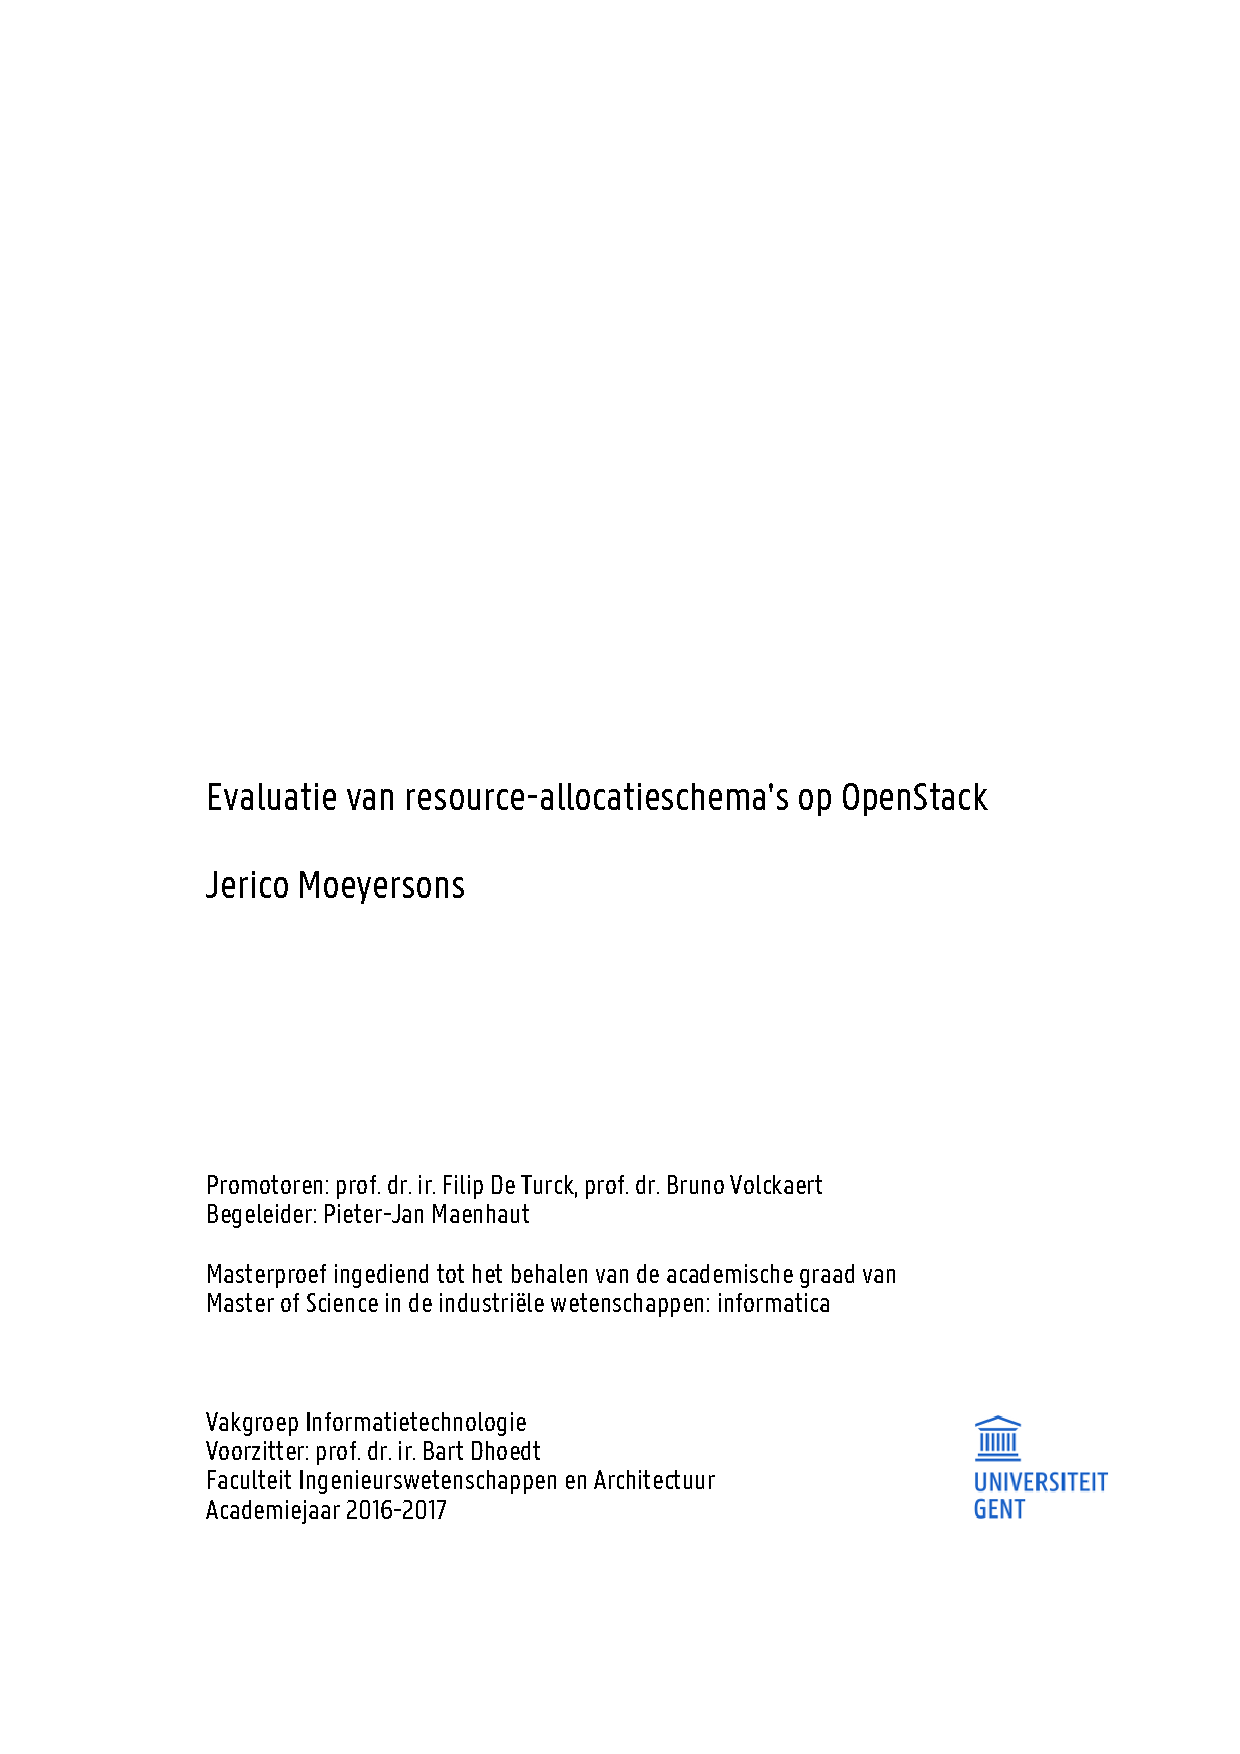
\includepdf{voorblad.pdf}                               % Front matter
\newpage\thispagestyle{empty}\mbox{}                    % White page
\thispagestyle{empty}    % Don't show page number

\begin{center}
\textbf{Dankwoord}
\end{center}

Na een intensieve periode van vijf maanden heb ik de laatste hand gelegd aan deze masterproef. Op verschillende vlakken heb ik nieuwe elementen binnen de wondere wereld van de informatica kunnen ontdekken. Daarom wil ik aan een aantal personen een welgemeende dankjewel zeggen om mij steeds te steunen tijdens het maken van deze masterproef.\\

Allereerst wil ik mijn promotoren, prof. dr. ir. Filip De Turck en prof. dr. Bruno Volckaert, bedanken voor het vertrouwen, de steun, de tips en de feedback. Ook mijn begeleider, de heer Pieter-Jan Maenhaut wil ik hartelijk bedanken voor de steun, de vele tips en uitgebreide feedback. Daarnaast wil ik ook mevrouw Leen Pollefliet bedanken voor de vele tips die ik nuttig heb kunnen gebruiken tijdens het schrijven en presenteren van deze masterproef. Vervolgens wil ik ook mijn vriendin, Lynn Haentjens, hartelijk bedanken om mij steeds te steunen in deze periode alsook voor het leveren van grammaticale feedback. Ten slotte wil ik ook mijn ouders bedanken voor de geleverde steun tijdens deze periode.\\

Om te eindigen met mijn dankwoord wil ik ook nog een aantal vrienden, namelijk Cédric Reyniers, Maxim Ronsse en Simon Vermeersch, bedanken voor de aangename middagpauzes, de relevante en ook de minder relevante gesprekken.\\
\\
Bedankt allemaal!\\
Jerico Moeyersons                            % Word of thanks
%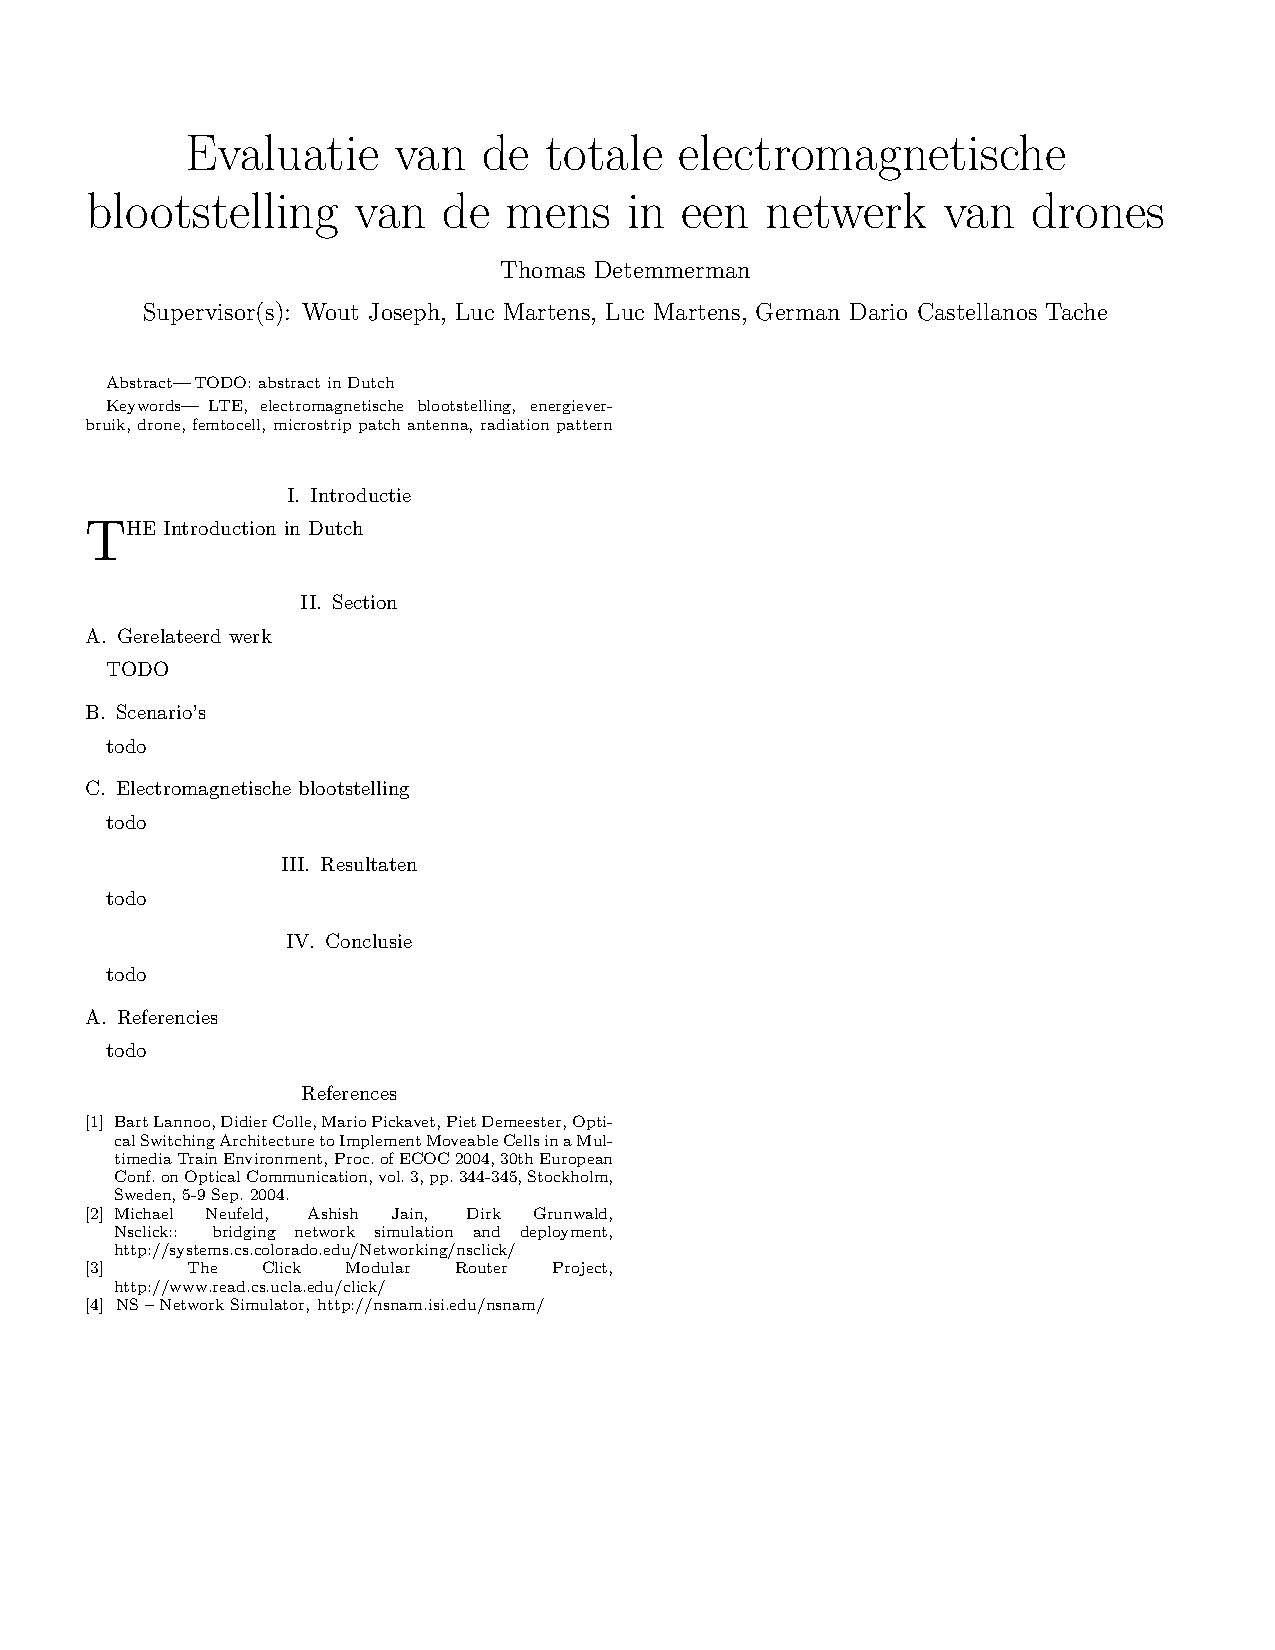
\includepdf[pages=-]{abstracts/extendedabstract.pdf}   % Extended Abstract
\tableofcontents                                        % Table of Contents
\listoffigures                                          % List of figures
\addcontentsline{toc}{chapter}{List of Figures}         %list "list of figures" in 'table of contents"
\listoftables                                           % List of tables
\addcontentsline{toc}{chapter}{List of Tables}          %list "list of tables" in "table of contents"
\listoflistings                                         % List of listings (code fragments)
\addcontentsline{toc}{chapter}{List of Listings}        %list "list of listings" in "table of contents"



%-------------------------------- acroniemen

\newacronym{UABS}{UABS}{Unmanned Arial Base Station}
\newacronym{EIRP}{EIRP}{equivalent isotropic radiation power}
\newacronym{UE}{UE}{User Equipment}
\newacronym{IEC}{IEC}{International Electrotechnical Commission}
\newacronym{SAR}{SAR}{Specific Absorption Rate}
\newacronym{whipp}{WHIPP}{WiCa Heuristic Indoor Propagation Prediction}
\newacronym{DL}{DL}{downlink}
\newacronym{UL}{UL}{uplink}
\newacronym{LTE}{LTE}{Long-Term Evolution}
\newacronym{FDD}{FDD}{Frequency Division Duplex}
\newacronym{TDD}{TDD}{Time Division Duplex}
\newacronym{ICNIRP}{ICNIRP}{International Commission on Non-Ionizing Radiation Protection}
\newacronym{LOS}{LOS}{line of sight}
\newacronym{NLOS}{NLOS}{non line of sight}
\newacronym{Exp Opt}{Exp. Opt.}{exposure optimized}
\newacronym{PwrC Opt}{PwrC. Opt.}{power consuption optimized}
\newacronym{WHO}{WHO}{World Health Organization}
\newacronym{FCC}{FCC}{Federal Communications Commission}
\newacronym{USA}{USA}{United States of America}
\newacronym{IOT}{IoT}{Internet of Things}
\newacronym{UAV}{UAV}{Unmanned Aerial Vehicle}
\newacronym{EU}{EU}{European Union}
%--------------------------------- woordenlijst
\newglossaryentry{isotropicradiator}{
	name = equivalent isotropic radiator,
	text = equivalent isotropic radiator,
	description = A theoretical source of electromagnetic waves which radiates the same intensity for all directions
}

\newglossaryentry{spuriousradiation}{
	name = spurious radiation,
	text = spurious radiation,
	description = According to the thefreedictionary.com: Any emission from a radio transmitter at frequencies outside its frequency band. Also known as spurious emission
}

\newglossaryentry{RRP}{
	name = RRP,
	text = RRP,
	description = RRP is an abreviation used in this paper to indicate an extension on EIRP and stands for Real Radiation Pattern. An RRP value indicates the power (in dBm) for a certain location unlike an EIRP where the power (in dBm) is independent of the location
}

\newglossaryentry{power flux density}{
	name = power flux density,
	text = power flux density,
	description = Magnitude of power ($W$) that travels through a curtain area ($m^2$)
}

\newglossaryentry{thermoregulatory capacity}{
	name = thermoregulatory capacity,
	text = thermoregulatory capacity,
	description = The capacity of an organism to regulate body temperture
}

%\printglossary[type=\acronymtype,title={Lijst van acroniemen}]
%\addcontentsline{toc}{chapter}{\textcolor{maincolor}{Lijst van acroniemen}}
%\printglossary
%\addcontentsline{toc}{chapter}{\textcolor{maincolor}{Verklarende woordenlijst}}





\printglossaries

%
% Include the main chapters of the thesis below
%
\mainmatter                                             % arabic page numbers
\pagestyle{headings}                                    % page numbers and subtitle in header
% Inspirerende caption 
%
%\begin{savequote}[0.55\linewidth]
%	``If you think you've seen this movie before, you are right. Cloud computing is based on the time-sharing model we leveraged years ago before we could afford our own computers. The idea is to share computing power among many companies and people, thereby reducing the cost of that computing power to those who leverage it. The value of time share and the core value of cloud computing are pretty much the same, only the resources these days are much better and more cost effective.''
%	\qauthor{\textasciitilde David Linthicum, author of Cloud Computing and SOA Convergence in Your Enterprise: A Step-by-Step Guide}
%\end{savequote}

\chapter{Introduction}
\label{chap:intro}

\section{Outline of the issue} %1p
\label{sec:issue}



% inspiratie kan je hier ook nog vinden:
% PREDICTION AND COMPARISON OF DOWNLINK ELECTRICFIELDAND UPLINK LOCALISED SARVALUES FOR REALISTIC INDOORWIRELESS PLANNING
Society is constantly getting more and more dependent on electronic communication. On any given moment in any given location, an electronic device
can request to connect to the bigger wireless network. Devices need more then ever to be connected, starting from small IOT sensors up to self-driving cars
which needs to be supported by the existing infrastructure. 

Once again it becomes clear why we're on the eve of a new generation of cellular communication named 5G. 
This new technology is capable of handling millions of connections every square meter %to do: klopt deze hoeveelheid want lijkt wel heel veel.
while satisfying only a few microseconds of a delay and providing connections up to 10Gbps \cite{5GFeatures}.

Also in exceptional and possibly life-threatening situations, we rely on the cellular network. For example during the terrorist attacks in Zaventem, a Belgian city.
Mobile network operators saw all telecommunications drastically increasing causing moments of contention. Some operators decided to temporarily exceed the exposure limits in
order to handle all connections. \cite{baseZaventem}

Electromagnetic exposure can however not be neglected. Research shows how exesive electromagnetic radiation can cause diverse biological side effects \cite{bioeffects}.
Because of public concern, the World Health Organization had launched a large, multidisciplinary research effort which eventually concluded that there was no sufficient evidence that confirmed 
that exposure to low level electromagnetic fields harmfull is \cite{WHO}. Nevertheless remains the public very concerned about potetial health risks.

\section{Objective}
\label{sec:objective}

In this master dissertation the electromagnetic exposure of  a user is investigated taking all prominent sources into account which include the user's own mobile device, basestations
and other users their \gls{UE}.

In order to determine the magnitude of exposure to which users in a certain area are exposed, various values need to be known. 
Not only the used technology but also the position of users and basestations need to be known. 
To make this research possible, an existing planning tool is used which gives insight in users and basestation distributions. Bitrates of idividual users, power useage of 
the different electronical devices and which basestations handels which users. The tool describes in other words a fully configured network.
In this way, all needed parameters will be known.

The electromagnetic exposure will then be analysed by applieing the tool in different scenarios. During the simulations
it is investigated how various input variables influence the network.

The calculation of electromagnic exposure originating from base stations is discussed in variously discussed in litterture. Papers who convert electromagnetic exposure
 into a single value is rather limited.
Not only how electromagnetic exposure behaves but also related values like power consumption or even coverage.



\textbf{research question 1:} How can a \gls{UABS} network be optimized to minimize global exposure and overal power consumption? What are the effects on the network?\\

\textbf{research question 2:} What are the advantages and disadvantages of a model as described in research question 1 compared the the already existing pahtloss oriented model.\\

\textbf{research question 3:} How does the \gls{UABS} fly height influence uplink and downlink exposure?


%todo: onderstaande tekst (in commentaar) is een letterlijke copy van J10-RDP. Het is hier gezet als referentie. Moet nog correct verwoorden:
%In this paper, prediction algorithms are created to
%simulate and visualise electric-field strengths due to
%downlink traffic and localised SARvalues due to uplink
%traffic. Downlink exposure are expressed in terms of
%whole-body exposure due to the electric-fields E originating
%from the base stations or APs, whereas uplink
%exposure are expressed in terms of localised SAR10g
%[SAR in 10 g of tissue(8)] values due to the mobile
%device’s transmitted signal. To

\section{Structure}
\label{sec:structure}

TODO: update this section

The following chapter \ref{chap:stateoftheart} exists of several succesive sections explaining how the electromagnetic exposure of a single human being is calculated. The first section \ref{sec:calculatingexposure}
explains how the exposure is calculated between a user and a single femtocell. Section \ref{sec:combiningexposure}  defines how to combine all exposures from the different femtocells towards a single users.
Finaly, section \ref{sec:radiationpatterns} explains how directional antenna's are taken into account.


\chapter{State of the art}
\label{chap:stateoftheart}

\section{Deployment tool for an UAV network}
\label{sec:stateoftheart:deploymenttool}

Calculating electromagnetic exposure requires knowledge about the area. The position of base stations need to be know,
 the transmission power used by the antenna and how far is the user separated from this base stations are only a few parameters
 that have to be considered.

The WAVES research group at UGent has developed a deployment tool for disaster scenarios with the aid of UAVs \cite{J2}.
The idea of this  UAV-aided emergency network is that in case of a disaster, the existing network might be damaged and won't be able 
to handle all users who are trying to reconnect to the backbone network. 
The tool makes a fast deployable network possible by attaching femtocells to UAVs, so-called \gls{UABS}s.
The tool will orchestrate the \gls{UABS}s over the disaster area. This tool is thus a suitable starting point and works as follows:

%The optimal placement for each \gls{UABS} needs to be defined to make sure that as many users as possible are properly reconnected to the backbone network while satisfying certain restrictions. 
%To make these calculations as realistic as possible the architecture of the several buildings present in the area is described in a shapefile. 
%A deployment tool calculates the optimal position of the \gls{UABS} by taking the 3D models of the building into account along with some femtocell specifications and user distribution. This deployment tool is developed by the WAVES research group, a department within Ghent University.

The deployment tool will try to calculate the optimal placement for each \gls{UABS} and requires therefore a description of the area where the UAV-aided network needs to 
be deployed. This is done with the use of so-called shape files. Theses files contains tree dimensional descriptions of the buildings present in the area and are
key values in approaching results as realistic as possible. Furthermore, the tool also requires a time period and a configuration file containing technical specifications of the type of \gls{UABS} that is being used. 
The tool will thereafter randomly distribute users over the area and assigns a certain bitrate to them. \\
\\
In a second phase, the optimal position for each \gls{UABS} is calculated. This is done by trying to locate a \gls{UABS} above each active user. Two options are possible.
If a flying height is defined, a base stations is placed above each user at the given height, unless a building is obstructing it's location. Then, no base station will be located above that user.
If no flying height is given to the tool, the base station is located 4 meters above the outdoor user or 4 meters above the building where the indoor user resides. 
The later is only allowed if the suggested height remains below the given maximum allowed height. \\
\\
Finally, all  \gls{UABS} are sorted on wether they were active or not, followed by the increasing pathloss from each \gls{UABS} to that user.
So the algorithm starts by checking for each active \gls{UABS} if it can cover the user. If this is the case, the user will be connected to this \gls{UABS}. If not,
the second active base station with a (slightly) worse pathloss is considered. If no active base station is suitable, inactive \gls{UABS} are considered. The user remains uncovered if no \gls{UABS}
is found. The reasoning behind first only considering base stations that are already active is the hight cost that comes along with each drone. \\
\\
Up till now, the tool has only calculated some suggestions. The effective provisioning is done in the fourth phase where drones are sorted by the ammount of users it covers. As long as \gls{UABS}
are available in the facility where they reside, \gls{UABS} are provisioned and its users are marked as covered.


\section{Electromagnetic exposure}

\subsection{Electromagnetic field radiation} % (fold)
\label{sub:emf}
People in a telecommunication network are exposed to far field electromagnetic radiation originating from base stations and other \gls{UE}. 
Network planners need to make sure that the the electromagnetic fields (expressed in V/m) does not exceed limitations enforced 
by the government. These limits are location dependent. The european union recommend the guidelines as defined by the \gls{ICNIRP} which limits electromagnetic exposure to 61 V/m.
Each european country needs to decide for themselves which limitations to enforce. Belgium for example delegated this responsibility to Flanders, Brussels and Wallonia \cite{J23}.

The used deployment tool is applied in Ghent, a Flemish city in Belgium. The standards defined by the Flemish government is therefore applicable.
They state that in the 2.6 Ghz frequency band, an individual antenna can't exceed 4.5 V/m and the cumulative sum of all fixed sources 31 V/m \cite{S13_normenBelgie}.

\subsection{Specific Absorption Rate}

\gls{SAR} represents the rate that electromagnetic energy is absorbed by human tissue with the thermal effect as it's most important health consequence.
The volume of this tissue is typically 1g or 10g. The Federal Communications Commission of the United States defines regulations based on 1g tissue (indicated as $SAR_{1g}$) 
while the European Union handles the 
10g model ($SAR_{10g}$). $SAR$ values can further be categorized based on the area it covers. 
A first one is whole body \gls{SAR} ($SAR^{wb}$) which is the average absorbed radiation over the entire 
body. The second type is more precisely. Localized \gls{SAR}-values cover only  a part of the human body like the head.
The \gls{ICNIRP} has concluded that the threshold effect for $SAR^{wb}_{10g}$ is at 4 W/kg meaning that any higher absorption rate would overwhelm the thermoregulatory capacity of the human body.
Whole body values between 1 and 4 W/kg increases the temperature of human body less then 1°C which is proven not to be harmful for a healthy human being\cite{J24}.
Thereafter, a safety margin is introduced to tackle unknown variables like experimental errors, increased sensitivity for certain population groups and so on. 
This results in a whole body $SAR_{10g}$ of $0.8 W/kg$ and $2 W/kg$ for localized $SAR_{10g}$ at head and torso area \cite{J23}.

%todo: de 10g slaat al op localized, vandaar dat het maar 10g is, anders is het whole-body
%todo: we kunnen niet sar10gmax gebruiken want This means that the SAR calculations will be worst-case and possibly an overestimation of the real localised SAR. (herwoorden voor plagiaat)
%Human exposure caused by downlink traffic is a not negligible asset. However, telecommunications is not a one-way street. When connecting to a UMTS network, also uplink data caused by the \gls{UE} should be considered.
%\gls{UE} generates, just like femtocells, electromagnetic waves to which a user is exposed. A part of this radiation goes to the femtocell, another part enters the body of its user. How much electormagnic strenghts enters the body is defined as \gls{SAR} and is measured with 10g biological tissue which represents the human skin. This value will from now on be expressed as $SAR_{10g}$. 
%A mobile device induces two types of exposure: local and whole-body. 

\subsection{Related work} % (fold)
\label{sub:general}
The goals of this master dissertation is the investigation of electromagnetic exposure considering all sources. Three types of sources are considered: electromagnetic radiation 
caused by basestations, near field radiation from the users own device and far field radiation originating from other users their equipment. This electromagnetic radiation is thereafter
absorbed by the human body which will be expressed in \gls{SAR} values.

Several papers exist calculating exposure originating from certain sources but very limited research has been done covering the whole picture.
In \cite{J6_originalExposureFormula} is described how electromagnetic radiation of several WiFi access points is being calculated. The authors of \cite{J1} used this knowledge 
to investigate electrmangetic exposure originating from basestations in a more outdoor environment. \cite{J10_RDP, J10.1} addresses the fact that 
also \gls{UL} traffic from the user's device should be considered. They therefore investigated indoor exposure. They did not only consider the electromagnetic radiation
but also how much is absorbed by the body wich will be expressed as specific absorption rate. Since the authors only covered voice calls,
uplink SAR was expressed in localized SAR values while the downlink traffic is expressed in whole body SAR. With the advent of 5G, paper \cite{J17_kuehn2019modelling} has been 
published describing how localized SAR values are achieved from all sources. More precisly: all mobile phones and all basestations in the network after which they converted the electromagnetic 
exposure to localized SAR values.
Finally, \cite{J22_plets2015joint} describes how both \gls{UL} and \gls{DL} traffic can be converted in whole body SAR values making it possible to achieve an overall picture. They applied this formula 
however only for the user's own device.

In a realistic network like the used deployment tool, some users are calling while annother part is using other type of telecommunication services like browsing the web.
Therefore, all absorbed electromagnetic exposure should be expressend in whole body SAR while still covering all sources.

\section{Optimizing towards electromagnetic exposure and power consumption}
\gls{UABS}s are drones with femtocell base stations attached to it. Drones can remain in the air for only a limited time, which is certainly 
the  case when also an antenna needs to be connected to the battery of the its carrier. It is therefore
interesting to not only considering electromagnetic exposure of the user but also the power consumption that comes with it. 
However an increasing transmission powers of an antenna comes with an increasing electromagnetic exposure, this is not the case considering
both values for an entire network. In fact, the autors from \cite{J1}  prove that both become inversely equivelent.

If a network is optimized towards power consumption, less drones will be provisioned radiating at higher power levels. This is because not only 
the transmission power is considered but also the power needed to keep the drone in the air. Therefore, it is cheaper to cover a user by 
increasing the antenna's transmission power of an already activated drone nearby as it therefore prevents the power cost of a new drone.
By increasing the transmission power, also the electomagnetic exposure will increase for users closer to that drone. An exposure optimized
network will therefore faster decide to power up a new drone.

todo: geen grid maar per user--> methodology

\section{Technologies}
\subsection{Type of drone}

Section \ref{sec:stateoftheart:deploymenttool} describes how femtocell antennae will be connected to helicopter drones. Two types of 
drones are considered in \cite{J2}: an off-the-shelf drone affordable by the generic public and a more expensive drone. The results in \cite{J2}
show that the second type will require less drones to cover the same number of users and will last longer in the air. The research in this paper
will therefore be done with the usage of the second type. A technical overview of this drone is given in table \ref{table:dronespecs}.

\begin{table}[h!]
\centering
\begin{tabular}{|l|c|l|}
\hline
 parameter          & value         \\    \hline
 Carrier power      & 13.0 A \\
 average carrier speed           & 12.0 m/s       \\ 
 Average carrier power usage    & 17.33 Ah      \\ 
 Carrier battery voltage        & 22.2 V \\ \hline
\end{tabular}
\caption{specifications for the used drone.}
\label{table:dronespecs}
\end{table}

\subsection{LTE}
The tool make usage of \gls{LTE} which is by the general public better known as 4G which allows better \gls{UL} and \gls{DL} data speeds 
compared to its predecessors and is based on an all IP architecture. LTE can cover macrocells supporting cell sizes ranging from 5 km up to 100 km. 
These type of antennae are usually attached to transmission towers along highways or on top of buildings. LTE supports however also smaller cells like
femtocells covering only a few hundred meters. They are therefore more portable, require less energy and won't require a telecommunication operator because
of it's simplicity. Femtocell base stations are therefore used by the deployment tool.
Further, \gls{LTE} also support both \gls{FDD} and \gls{TDD}.

\gls{FDD} makes simultaneous \gls{UL} and \gls{DL} traffic possible by assiging different frequencies within the frequency range 
to both data streams. A small guardband is used between \gls{UL} and \gls{DL} directions in other to prevent interference.

\gls{TDD} allows  \gls{UL} and \gls{DL} by splitting the time domain. Meaning that both traffic directions use the same frequency and therefore
alternately (in time) use the frequency spectrum. A small time interval is used to prevent interference in case of a slightly bad timed synchronization.

This master dissertation will make usage of \gls{FDD}.

\subsection{Type of antenna} % (fold)

An important part of this master dissertation is the type of antenna that will be used by the femtocell base stations. The deployment tool makes use
of drones that will position the femtocell base stations in the right position.  Using conventional 
sector antennae, as used by traditional terrestrial transmission towers, would be to complicated for a simple drone. 
The characteristics of microstrip antennae will therefore be investigated.

Microtstrip antennae provide several advantages compared to traditional antennae \cite{J13_singh2011micro, J14_antennadesign}. Microstrip antennae
are lightweight, low in cost and thin causing them to be more aerodynamic which is  a useful feature since the antennae will be attached
to flying drones.

A basic microstrip antenna like figure \ref{fig:basicpatchantenna} consists out of a ground plane and
a radiating patch, both separated with a dielectric substrate. Several variations exist like microstrip patch antenna, microstrip slot antenna and printed dipole antenna which
has all similar characteristics. They are all thin, support dual frequency operation and they all have the disadvantage that they 
will transmit at frequencies outside the aimed band which is also known as
\gls{spuriousradiation}. The microstrip patch and slot antenna support both linear
and circular polarization while the printed dipole only support linear polarization. Further is the fabrication of a microstrip patch antenna considered to be the easiest of its competitors. 

\begin{figure}[H]
\centering
  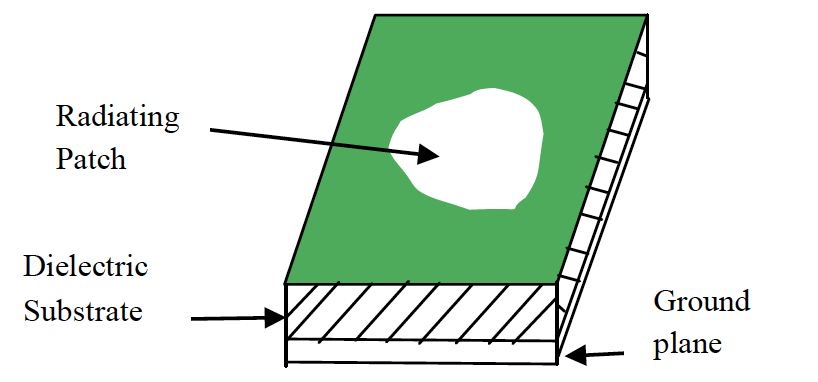
\includegraphics[width=\textwidth/2]{../images/patchantenna.png}
  \caption{General design of a microstrip antenna}
  \label{fig:basicpatchantenna}
\end{figure}

The microstrip antenna requires besides the groundplane, dielectric substrate and the radiation patch also a feed line. Several feeding techniques exists of which the most popular are: coaxial probe feeding, microstrip line and apeture coupling. %and Microstrip Patch Antenna
(todo: more refs? gebruik nummer twee van J13 (p2))

A first feeding method is with the usage of a coaxial cable where the outer conductor is attached to the ground plane and the inner conductor to the radiations patch. Modelling is however difficult, escpecially for thic substrates as will be used in this master dissertation.
A second option is the usage of a microstrip line. This type of feeding is much easier to model since the microstrip line can be seen as en extension of the radiating patch.
A disadvantage is the increased \gls{spuriousradiation} which limits bandwith.
A third is proximity coupling which has the largest bandwidth and low \gls{spuriousradiation}. It consist however of two dielectric substrates causing the overall thickness
of the antenna to increase as well as it's fabrication difficulty.
(todo: tekst te weinig, bespreek ook apperture coupled attenna (zelfde paper als de rest))

The increasing usage of the microstrip patch antennae can be explained by it's easy fabrication and lightweightness and therefore knows a widespread application in the millitary, global possitioning systems, telemedicine, WiMax applications and so on.
The authors of \cite{J13_microstripadvantages} also state that some of the disadvantages like lower gain and power handling can be solved with the usage of an array configuration.

The radiating patch is usually made of a thin layer of either gold or copper \cite{J14_antennadesign,J15_antennadesign}
and can be any form. However, shapes besides a circle or rectangle would require large numerical computation \cite{J14_antennadesign}.
A simple rectangular shape will thus be used.
Further is also the dielectric constant of the substrate important which typically varies between 2.2 and 12. Finding a good dielectric depends on how the antenna will used. A lower
dielectric constant with a thick substrate will result in better performance, better efficiency and larger bandwidths  \cite{J15_antennadesign}.
On the other hand, a larger dielectric constant reduce de dimensions of the antenna \cite{J14_antennadesign}
which is also useful when attaching the 
antenna to a limited surface. Glass as a dielectric substrate with a constant of 4.4 will therefore be used.
\chapter{Scenarios}
\label{chap:scenarios}
The tool supports multiple configurations and the tool will behave differently for most configurations. Three main scenarios 
will be investigated, order based on the network complexity. Within each scenario, different configurations will be applied.
For the first scenario, only one user with one drone will be present in the network. The network will thereafter be expanded
for multiple users but with still only one drone available. Eventually, that last restriction will be dropped meaning 
that the third scenario covers multiple users with unlimited number of drones. Table \ref{table:defaultconf} show the default configuration which 
always applicable unless mentioned otherwise.

\begin{table}[!htb]
\centering
\begin{tabular}[t]{ll}
        \toprule
        \multicolumn{2}{l}{\textbf{broadband cellular network}} \\
        \hline
        \hspace{3mm}  technology        & LTE     \\
        \hspace{3mm}  frequency         & @ 2.6 GHz \\
        \hline
        \multicolumn{2}{l}{\textbf{Carrier}} \\
        \hline  
        \hspace{3mm}  Carrier power        & 13.0 A   \\
        \hspace{3mm}  average carrier speed        & 12.0 m/s \\
        \hspace{3mm}  Average carrier power usage      & 17.33 Ah    \\
        \hspace{3mm}  Carrier battery voltage       & 22.2 V \\
        \hline
        \multicolumn{2}{l}{\textbf{femtocell antenna}} \\
        \hline  
        \hspace{3mm}  maximum $P_{tx}$          & 33 dBm   \\
        \hspace{3mm}  antenna  direction        & downwards (az: \ang{0}; el: \ang{90})    \\ 
        \hspace{3mm}  gain                      & 4 dBm   \\ 
        \hspace{3mm}  feeder loss               & 2 dBm   \\ 
        \hspace{3mm}  implementation loss       & 0 dBm   \\
        \hspace{3mm}  radiation pattern         & \shortstack[l]{\gls{EIRP} or \\ microstrip patch antenna } \\
        \hspace{3mm}  height                    & 100m  \\
        \hline
        \multicolumn{2}{l}{\textbf{\gls{UE} Antenna}} \\
        \hline 
        \hspace{3mm} height                     & 1.5m from the floor       \\ 
        \hspace{3mm}  gain                      & 0 dBm   \\ 
        \hspace{3mm}  feeder loss               & 0 dBm   \\ 
        \hspace{3mm}  radiation pattern         & \gls{EIRP}  \\
        \toprule
\end{tabular}
\caption{Overview of default configuration values.}
\label{table:defaultconf}
\end{table}

%%%%%%%%%%%%%%%%%%%%%%%%%%%%%%%%%%%% scenario 1
\section{A single user}
\label{sec:s1}

This first scenario will investigate how $SAR_{10g}$ is influenced in an isolated environment meaning there is nor influence 
from other base stations nor other \gls{UE}. The tool will provision one single drone and position it directly above the user.
These results will however depend on the position of the user. If the randomly generated location of the user is indoor, 
the flying height of the drone might obstructed by the building where the user resides, causing the user to be uncovered. If this is not the case,
the expected altitude of the user is half of the height of the building meaning that the user would be closer to the \gls{UABS} as 
if he would have been outdoors. For a more consistent result, the user will therefore be positioned outside when systematically 
increasing the fly height. Another considered variable is the transmitting power of the \gls{UABS}.

This scenario deducted with two type of antennas. First, an \gls{isotropicradiator} will be used and thereafter a realistic antenna.
It is expected that after the introduction of an realistic antenna, the user coverage will decrease.

The scenario consist of two groups with each 3 series of simulations. The first group is with an \gls{isotropicradiator} and the second 
will be identical but with a realistic radiation pattern. The first series of simulations
investigates $SAR_{10g}$ and power consumption of the network for a variable flying height but a fixed maximum transmission power of 
33dBm as defined in \cite{J2}. The second series 
investigates the minimal require transmit power by the used antenna for a fixed flying height of 100 m 
which is the proposed flying height by \cite{J2} but with a variable transmit power of the base station.

The user gets a fixed position. The exact location doesn't matter as long as it is outside. For this experiment is choses for the 
`Koningin Maria Hendrikaplein', a square just next to the train station of Ghent.  Doing so will force the \gls{UE} 
to always be at the same height of 1.5 meters. The conclusions will be based on $SAR_{10g}$, power consumption and transmission power.
These output values depend on fly height and type of antenna. An overview can be found in table \ref{table:confOverviewScenario1}

\begin{table}[!htb]
    \begin{minipage}{.5\linewidth}
      \centering
        \begin{tabular}{|l|c|l|}
        \hline
        x possition user               & 3.711198       \\    
        y possition user               & 51.036747          \\ 
        shadow margin user             & -3.0398193315963473 \\
        height of the \gls{UE}         & 1.5m                      \\ 
        frequency                      & 2600Hz                   \\ 
        antenna  direction             & downwards (az: \ang{0}; el: \ang{90})    \\ 
        \hline
        \end{tabular}
    \end{minipage}%
    \begin{minipage}{.5\linewidth}
      \centering
            \begin{tabular}{|l|l|}
            \hline
            Input variables                & Output variables          \\   \hline 
            type of antenna                & $SAR_{10g}$               \\ 
            fly height                     & power consumption             \\ 
               &   \\ 
            \hline
            \end{tabular}
    \end{minipage} 
        \caption{Overview of the configuration.}
        \label{table:confOverviewScenario1}
\end{table}


%%%%%%%%%%%%%%%%%%%%%%%%%%%%%%%%%%%% scenario 2


\section{Increasing traffic with only one drone available}
The previous scenario will be extended for an increasing amount of users. 

\begin{table}[!htb]
    \begin{minipage}{.5\linewidth}
      \centering
        \begin{tabular}{|l|c|l|}
        \hline
        todo               & todo        \\    
        todo               & todo\\ 
        todo               & todo                     \\ 
        frequency                      & 2600Hz                   \\ 
        \hline
        \end{tabular}
    \end{minipage}%
    \begin{minipage}{.5\linewidth}
      \centering
            \begin{tabular}{|l|l|}
            \hline
            Input variables                & Output variables          \\   \hline 
            type of antenna                & $SAR_{10g}$               \\ 
            fly height                     & power consumption             \\ 
            number of users                & user coverage            \\ 
            \hline
            \end{tabular}
    \end{minipage} 
        \caption{Overview of the configuration.}
        \label{table:confOverviewScenario2}
\end{table}

The $SAR_{10g}$, power consumption and user coverage will be investigated for an increasing amount of users ranging from 50 to 650 in steps of 50.
The only available drone will be positioned at the fly height of 100 m as recommended in \cite{J2}. For the second case, the same output variables are investigated 
for a varying fly height but with a fixed number of 224 users. This case will be applied in the city center of Ghent, assuming it is an average 
day at 5 p.m. which means it is rush hour resulting in the highest number of simmulatanious users for the day\cite{J2}. 
Both cases will be investigated for the two types of antennae: the fictional \gls{isotropicradiator} and the microstrip patch antenna.


%%%%%%%%%%%%%%%%%%%%%%%%%%%%%%%%%%%% scenario 3


\section{Increasing traffic with an undifend amount of drones}

\begin{table}[!htb]
    \begin{minipage}{.5\linewidth}
      \centering
        \begin{tabular}{|l|c|l|}
        \hline
        todo               & todo        \\    
        todo               & todo\\ 
        todo               & todo                     \\ 
        frequency                      & 2600Hz                   \\ 
        \hline
        \end{tabular}
    \end{minipage}%
    \begin{minipage}{.5\linewidth}
      \centering
            \begin{tabular}{|l|l|}
            \hline
            Input variables                & Output variables          \\   \hline 
            type of antenna                & $SAR_{10g}$               \\ 
            fly height                     & power consumption             \\ 
            number of users                & number of drones            \\ 
            \hline
            \end{tabular}
    \end{minipage} 
        \caption{Overview of the configuration.}
        \label{table:confOverviewScenario2}
\end{table}


When more drones are available, an optimization strategy can be applied. The tool checks the capacity of the basestations and decides thereafter
wich basestation the user should be connected to. The original algorithm checks all pahts between the user that need to be connected with 
all drones. Thereafter, the drones which path experience the least pathloss and still has the capacity to cover an addition user will be selected.
The authors from \cite{J1} proposed however annother optimization strategy which tries to minimize electromagnetic exposure and 
power consumption.

The input variables flying height, transmit power and number of users will be used to see how electromagnetic exposure, power consumption en number of drones are influenced for
different optimization strategies and type of antennas.

Since there is no fixed budget limitation, the number of drones are unlimited. The tool will therefore try to connect each user and
coverage will be expressed in number of drones required to cover as much users as possible instead of having a limited number of drones  
as in scenario and therefore has only a limited coverage expressed in percentage.
\chapter{Methodology}
\label{chap:methodology}


\section{Tool}
The goals 
\begin{figure}[h!]
\centering
  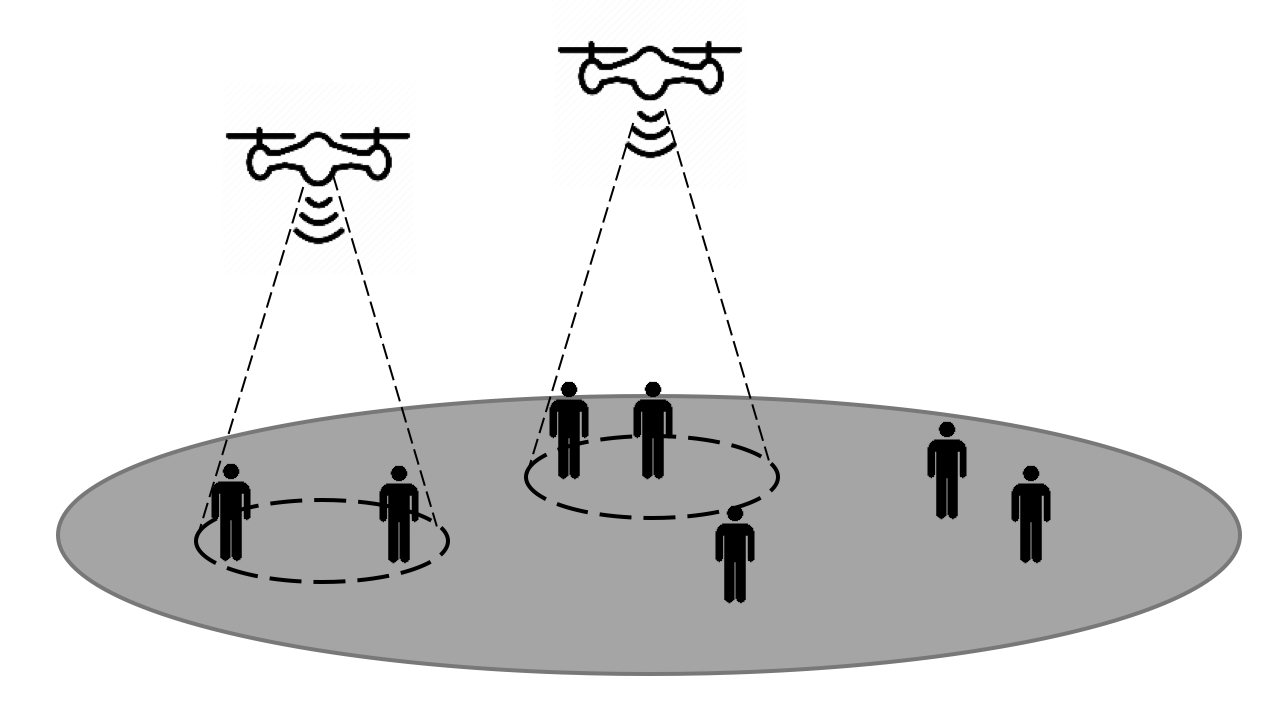
\includegraphics[width=\textwidth]{../images/generalIdeaIllustration.png}
  \caption{Design of the microstrip patch antenna.}
  \label{fig:antennadesign}
\end{figure}


\section{Electromagnetic exposure}
\subsection{Calculation of the total specific absorption rate} % (fold)
\label{sub:Calculationexposure}

The total whole body \gls{SAR} ($SAR^{wb}_{10g}$) of a user can be calculated by a simple sum of individual SAR values from the different sources.
Forumula \ref{eq:overallSARwb} was originally described in \cite{J17_kuehn2019modelling} for \gls{SAR} values induced into the head.
Using $SAR^{head}_{10g}$ would however result into incorrect conclusions since 
the position of the phone relative to the user is unknown. This is because the tool assigns a bitrate 
to a user depending on the service he is using
meaning that users in the network are not only calling but are able of using other services as well like browsing the web. 
The position of the phone can thus be next to the head but also in front of the user.
The induced electromagnetic radiation will therefore be expressed in function of the entire body.


\begin{equation} 
SAR^{wb,total}_{10g} = SAR^{wb,ul}_{10g} +  SAR^{wb,dl}_{10g} + SAR^{wb,neighbours}_{10g}
\label{eq:overallSARwb}
\end{equation}

The first parameter, $SAR^{wb,ul}_{10g}$, will indicate the absorbed electromagnetic radiation by the entire body originating from the user's own device
whereas the second parameter $SAR^{wb,dl}_{10g}$ will represent the absorbed electromagnetic radiation caused by all the base stations in the considered area.
The last factor, $SAR^{wb,neighborhood}_{10g}$, specifies the exposure of our user to \gls{UL} radiation from other mobile devices.

\subsection{Electromagnetic exposure caused by far-field radiation} % (fold)
\label{sub:Calculatingdownlinkexpsure}

The electromagnetic exposure to which people are exposed can be categorized in two groups. One of them is near-field radiation which is caused 
by the users own device and which will be discussed in \ref{sub:Uplinkexposure}.
The other type is far-field radiation and will be explained in this section. This kind of radiation is caused by radiators `far away'.
Examples of these types of radiators are \gls{UE} which belong to other people and \gls{UABS}s. 

\subsubsection{Electromagnetic radiation from a single source}
\label{sec:calculatingexposure}

To determine the total exposure of a single human being or even of the entire network, the electric-field $\vec{E}$ from a single radiator $i$ should be calculated.
The formula to determine this electromagnetic value $E$ (expressed in V/m) for a specific location $u$ is given in equation \ref{eq:singleexposure}.

\begin{equation}
E_i(u) = 10^{\frac{RRP(u) - 43.15 + 20*\log(f)- PL(u)}{20}}
\label{eq:singleexposure}
\end{equation}

\paragraph{frequency}
The used frequency in the formula above is denoted as $f$ and is expressed in Mhz. Since LTE is used, this value will be 2600.

\paragraph{Real Radiation Power and EIRP}
In the original formula of \ref{eq:singleexposure}, as it was described in \cite{J1, J6_originalExposureFormula}, 
is \gls{RRP} defined as \gls{EIRP}. An \gls{EIRP} is a radiation pattern generated by an \gls{isotropicradiator} which is
a theoretical source of electromagnetic waves that radiate with the same intensity in all directions. 
The formula to find this \gls{EIRP} value is described in \ref{eq:eirp}
where $P_t$ stands for the input power of the antenna, $G_t$ for the gain of the transmitter and $L_t$ being it's feeder loss.
\begin{equation}
EIRP = P_t + G_t - L_t
\label{eq:eirp}
\end{equation}
This formula, constructed out of different gains and losses, misses a factor when accounting for real life radiation patterns.
Therefore makes formula \ref{eq:singleexposure} usage of \gls{RRP} instead of \gls{EIRP} and can be defined as follows:
\begin{equation}
RRP(u) = EIRP - attenuation(u)
\label{eq:rrp}
\end{equation}
The attenuation for a user $u$ is given based on the angle between the main beam and the user. More details on how this can be implemented is described in \ref{subsec:implementationradpat}
Thereafter, the attenuation can simply be subtracted from the EIRP-value, when assuming that $attenuation(u)$ returns positive values.
\paragraph{path loss}
\label{subsec:pl}
At last, formula \ref{eq:eirp} requires the path loss (dB). In order calculate the path loss, an appropriate propagation model is required of which several exist.
The tool uses the Walfish-Ikegami model because it performs well for femtocell networks in urban areas \cite{J2}. %optioneel kan je hier dezelfde bron gebruiken als dat ze in thesis van de vorige gebruikten. Bron nummer 32
The chosen propagation model consists of two formulas depending on whether a free line-of-sight between the user and the base station exist or not. Both formulas expect a distance in kilometer. %bron?

\subsubsection{Combining exposure}
The electromagnetic exposure for a given location originating from different sources can be calculated with formula \ref{eq:totalexposure} (in V/m). $E_i$ stands for 
the electromagnetic exposure from source $i$ and
$n$ stands for all far-field radiators of a certain category which will either be \gls{UABS}s or \gls{UE} from other people.
$E_{tot}$ was originally calculated for each $x$ meters \cite{J1}. In the tool, the exact location of the users in known and $E_{tot}$ will thus 
only be calculated for locations where a user is positioned.
\begin{equation}
E_{tot} = \sqrt{\sum_{i=1}^{n} E_i^2}
\label{eq:totalexposure}
\end{equation}

\subsubsection{Converting far-field electromagnetic exposure to $SAR^{wb}_{10g}$}
\label{sub:convertDLtosarwb}

Formula \ref{eq:overallSARwb} expects that the electromagnetic radiation expressed into $SAR^{wb,dl}_{10g}$ and $SAR^{wb,neighbours}_{10g}$. The 
calculation for both values are in fact identical. The difference is the sources where the first one is for \gls{UABS}s and the second one for \gls{UE}.
Physically seen, they are both whole body SAR values induced by far-field radiation $SAR^{ff,wb}_{10g}$.

The electromagnetic radiation needs to be converted into $SAR^{ff,wb}_{10g}$. 
This conversion factor is based on Duke from the Virtual Family. Duke is a 34-year old male with  a weight of 72 kg, an height of 1.74 m and body
mass index of 23.1 kg/m \cite{J22_plets2015joint}. Research shows that the conversion factor for WiFi is $0.0028 \frac{W/kg}{W/m^2}$.
 Since WiFi, at a frequency of 2400 Mhz,
is very close to LTE, at 2600 Mhz, it is assumed in \cite{J22_plets2015joint} that this value is also applicable for \gls{LTE}.
This constant converts converts the \gls{power flux density} $S$ (with units $\frac{W}{m^2}$) to the required $SAR^{ff,wb}_{10g}$.
To make this possible, the electromagnetic radiation
from formula \ref{eq:totalexposure} (expressed in  $V/m$) should first be converted to the  \gls{power flux density} which formula 
\ref{eq:flux} before formula \ref{eq:convertion} can be applied.

\begin{equation}
S  = \frac{E^2}{337}
\label{eq:flux}
\end{equation}
\begin{equation}
SAR^{wb,dl}_{10g} = S * 0.0028
\label{eq:convertion}
\end{equation}

\subsection{Electromagnetic exposure caused by near-field radiation}
\label{sub:Uplinkexposure}
When a user is operating his device, a part of the \gls{UL} radiation will enters the user's body despite the fact that the 
 traffic is destined for the serving \gls{UABS}. So the 
 electromagnetic exposure won't be limited by \gls{DL} traffic from \gls{UABS}s or \gls{UL} traffic 
from other \gls{UE} but also from \gls{UL} traffic from his own device.

\subsubsection{Localized Specific Absorption Rate}

When assuming that all users hold their device next to their ear, a localized SAR-value for the head $SAR^{head}_{10g}$ can be calculated.
\gls{IEC} defines in IEC:62209-2 a maximum for a 10g tissue $SAR^{head}_{10g}$ as 2 W/kg and a maximum for a 1g tissue $SAR^{head}_{1g}$ as 1.6 W/kg.
Most countries, including Belgium, enforce the 10g model and will, therefore, be the point of reference for this master dissertation.
The $SAR^{head}_{10g}$ values are phone dependent. The reported values by companies of mobile devices are worst-case scenarios meaning that the 
values are measured when the phone is transmitting at maximum power. This is an understandable decision but won't result in a realistic scenario since 
modern cellular networks use power control mechanisms to prevent over radiation of a nearby device. \gls{UE} will therefore never use more energy than 
necessary to maintain a connection.
To compensate for this overestimation, the actual $SAR^{head}_{10g}$ of each user will be predicted. These will, however, remain an estimation since the 
position of the phone related too the head differs from user to user. For example, by holding the phone differently, a hand can absorb more or less 
electromagnetic radiation. TODO: bron. 
\begin{equation}
{SAR}_{10g} = \frac{P_{tx}}{P^{max}_{tx}} * {SAR}^{max}_{10g}
\label{eq:calculatesar}
\end{equation}
Equation \ref{eq:calculatesar} will be used to predict the actual $SAR^{head}_{10g}$  of a certain user with 
$P^{max}_{Tx}$ being the maximum transmission power for a phone which is in \gls{LTE} and UMTS 23 Dbm \cite{J11_maxTpxUE, J10_RDP}.
The actual transmitted power ($P_{tx}$), is calculated with equation \ref{eq:ptx} where $P_{sens}$
stands for the receiver sensitivity and $PL$ the path loss between sender and receiver.
\begin{equation}
P_{tx} = P_{sens} + PL
\label{eq:ptx}
\end{equation}
 
The $SAR^{max}_{10g}$ value is different for each mobile device. 
An average is calculated based on 3516 different phones from various brands using an German database \cite{SARDatabase} for which an overview can be 
found in fig. \ref{chart:germanDatabase}.
When the phone is positioned at the ear, an average of 0.7 $W/kg$ is found with a standard deviation of 0.25 $W/kg$ which are very similar 
results as in ref. \cite{j10.1.1}. The median of 0.67 is used.

%todo: schrijven dat het enigste verschil een std van 0.27 is?
%todo: j10.1.1 schrijft door de std van 0.25 dat er een onzekerheid van 40% is.
%todo: J10 en J10.1 rapoteert een sar max van 0.476. Update in het report is het een Nokia terwijl het bij ons voor de gemiddelde gsm is.


\definecolor{hous}{HTML}{3065c1}
\begin{figure}
  \begin{tikzpicture}
  \begin{axis}[
          ybar=-1cm,
          axis x line*=bottom,
          axis y line*=left,
          bar width=1cm,
          xlabel near ticks,
          height=8cm, width=\textwidth,
          ylabel={Percentage of mobile phones},
          xlabel={SAR},
          symbolic x coords={0.0--0.2,0.2--0.4,0.4--0.6,0.6--0.8,0.8--1.0,1.0--1.2,1.2--1.4,1.4--1.6,1.6--1.8,1.8--2.0},
          x tick label style={rotate=45, anchor=east, align=left},
          nodes near coords,
          nodes near coords align={vertical}      
          ]
          \addplot[hous,fill]  coordinates {(0.0--0.2,2)};
          \addplot[hous,fill]  coordinates {(0.2--0.4,16)};
          \addplot[hous,fill]  coordinates {(0.4--0.6,23)};
          \addplot[hous,fill]  coordinates {(0.6--0.8,24)};
          \addplot[hous,fill]  coordinates {(0.8--1.0,19)};
          \addplot[hous,fill]  coordinates {(1.0--1.2,8)};
          \addplot[hous,fill]  coordinates {(1.2--1.4,5)};
          \addplot[hous,fill]  coordinates {(1.4--1.6,2)};
          \addplot[hous,fill]  coordinates {(1.6--1.8,1)};
          \addplot[hous,fill]  coordinates {(1.8--2.0,0)};
      \end{axis}
  \end{tikzpicture}
  \caption{Distribution of how many phones belong to a certain SAR interval. Upper boundary not included}
  \label{chart:germanDatabase}
\end{figure}


\subsubsection{Whole body specific absorption rate}
The position of the phone relative to the user's body is however unknown. The tool assigns different bitrates to different phones implying 
that some users calling and therefore probably holding their phone next to their ear while another part is using other services like browsing the web.
The $SAR_{10g}$ caused by the user's \gls{UL} traffic will for this reason be expressed in function of the entire body.
For this reason expects formula \ref{eq:overallSARwb} that the specific absorption rate is expressed for the entire body instead of localized $SAR^{head}_{10g}$.
The conversion factors for Duke from the Virtual Family will be used again as which was already the case in \ref{sub:convertDLtosarwb}. This constant 
for WiFi is defined to be 0.0070 $\left(\frac{W/kg}{W}\right)$ \cite{J22_plets2015joint}.

\begin{equation} 
SAR^{wb,ul}_{10g} \left(\frac{W}{kg}\right) = 0.0070 \left(\frac{W/kg}{W}\right) * P_{tx} (W)
\label{eq:solve}
\end{equation}

\subsection{Defining an antenna}
\label{sub:definingAntenna}
A microstrip patch antenna is chosen because it allows easy production but more important it has a low weight 
and has a thin profile causing it to be very aerodynamic which is useful when attaching it to an \gls{UABS} \cite{J13_microstripadvantages}.

The dimensions of the antenna depend on the frequency it is operating and the characteristics of the used substrate.
The antennae will be radiating at a center frequency $f_0$ of 2.6Ghz. Each substrate has a dielectric constant $\epsilon_r$ representing 
the permittivity of the substrate and depends on the used material.
Substrates with a high dielectric constant and low height 
reduces the dimensions of the antenna
while a lower dielectric constant with a high height improves antenna performance. 
In this paper, a substrate like glass 
is chosen because of the higher dielectric constant of $\epsilon_r = 4.4$ compared to materials like teflon with only a dielectric 
constant of $\epsilon_r = 2.2$ \ref{J14_antennadesign}. 
Doing this in combination with an antenna height of 2.87 mm will decreases the dimensions of the entire antenna surface which comes in handy for the limited space on 
drones.

\begin{table}[h!]
\centering
\begin{tabular}{|l|c|l|}
\hline
 description            & symbol          & value         \\    \hline
 center frequency       & $f_0$           & 2600 Hz       \\ 
 dielectric constant    & $\epsilon_r$    & 4.4         \\ 
 heigt of the substrate & $h$             & 0.00287m    \\ \hline
\end{tabular}
\caption{Overview of configuration parameters}
\label{table:antennaparas}
\end{table}

The dimensions of the radiating patch can be calculated with the formulas from \cite{J14_antennadesign} and \cite{J15_antennadesign}
using the defined values in table \ref{table:antennaparas}. In that way, the width $W$ is calculated using formula \ref{eq:antennawidth}.

\begin{equation} 
W = \frac{c}{2*f_0*\sqrt{\frac{\epsilon_r+1}{2}}}
\label{eq:antennawidth}
\end{equation}
With $C$ being the speed of light, $f_0$ the center frequency of 2600 MHz and a dielectric constant $\epsilon_r$ of 4.4. This results 
in a width of 3.51 mm.

In order to find the length off the radiating patch, some other values need to be determined first. Formula \ref{eq:epsilonreff} will
calculate the effective dielectric constant ($\epsilon_{reff}$).
\begin{equation} 
\epsilon_{reff} = \frac{\epsilon_r+1}{2}+  \frac{\epsilon_r-1}{2} * \left(1+12*\frac{h}{W}\right)^{-\frac{1}{2}}
\label{eq:epsilonreff}
\end{equation}
This formula requires the width found in the previous formula along with the dielectric constant and substrate height from table \ref{table:antennaparas}.
This will result in a $\epsilon_{reff}$ of 3.91.

\begin{equation} 
L_{eff} = \frac{c}{2*f*\sqrt{\epsilon_{reff}}}
\label{eq:leff}
\end{equation}
Now formula \ref{eq:leff} is used to calculate effective length ($L_{eff}$) which result in 29.16 mm.

\begin{equation} 
\Delta L = 0.412*h*\frac{(\epsilon_{reff}+0.3)\left(\frac{W}{h}+0.264\right)}{\left(\epsilon_{reff}-0.258\right)\left(\frac{W}{h}+0.8\right)}
\label{eq:lenghtextension}
\end{equation}
Eventually, the lenght extension is found with formula \ref{eq:lenghtextension} by substituting the values from above.
Doing so determines that the $\Delta L$ equals 1.3071 mm.

Finally can the length of the patch be calculated using the expression: $L = L_{eff} - 2 * \Delta L$
which result in 26.55 mm.

The dimensions of the radiation patch are now known. The only remaining question are the dimensions of the ground plane and dielectric substrate to which the 
radiation patch is attached. The transmission line model is in fact only applicable for an infinite ground plane but it has been proven that similar results
can be achieved if the ground plane's dimensions are bigger then the patch by approximately 6 times the height of the dielectric substrate \cite{J14_antennadesign,J15_antennadesign}.

\begin{equation} 
L_{g} = 6 * h + L
\end{equation}
\begin{equation} 
W_{g} = 6 * h + W
\end{equation}
Therefore, should the length of the ground plane $L_{g}$ be at least 0.0438m and a width of $W_{g}$ 0.0524m.
A schematic overview of how the antnena will look like is given in figure \ref{fig:antennadesign}.
\begin{figure}[h!]
\centering
  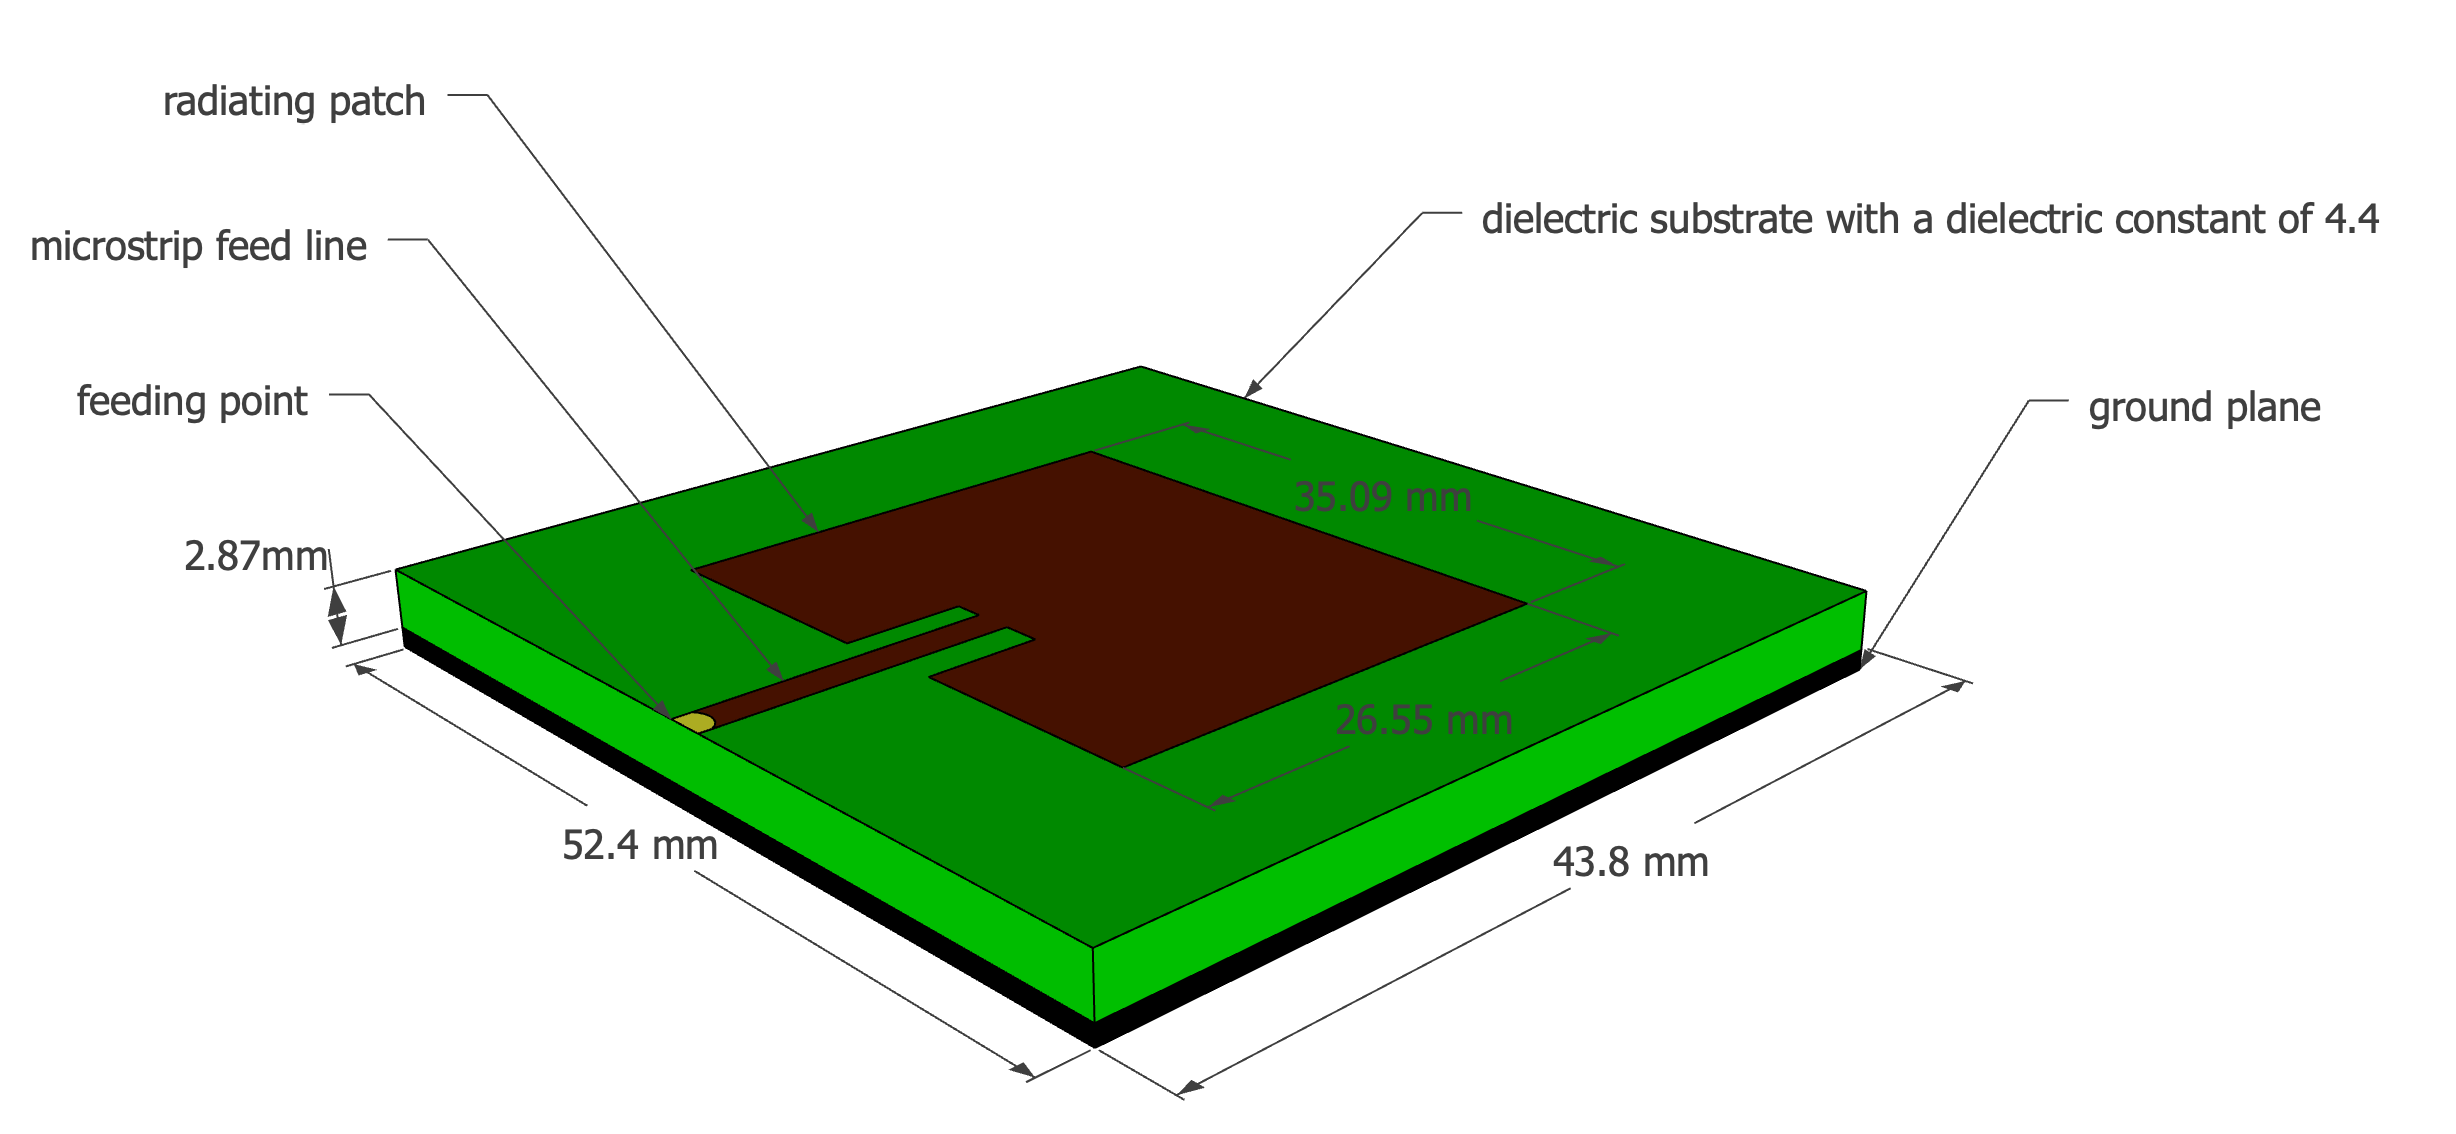
\includegraphics[width=\textwidth]{../images/MicrostripAntenna.png}
  \caption{Design of the microstrip patch antenna.}
  \label{fig:antennadesign}
\end{figure}

\subsection{Radiation pattern}
Mathlab is able to generate the radiation pattern for the this microstrip patch antenna.
The code in  listing \ref{c:mathlabradpattern} starts with defining the dielectric substrate which will be glass with a dielectric constant
of 4.4 and a height of 0.00287m. Thereafter, is the microstrip patch antenna generated with the \verb|width| and \verb|length| being the dimensions
of the radiation patch and the \verb|GroundPlaneLength| and \verb|GroundPlaneWidth| the dimensions of the ground plane and dielectric substrate.
The \verb|FeedOffset| is the relative offset from the center where the radio frequency power is fed to the radiating patch which will here be
at the edge. This  is in figure \ref{fig:antennadesign} indicated with the yellow dot. At last, the \verb|dielectric|-object is substituted into the 
\verb|patchMicrostripInsetfed|-object.

Generating the pattern is done with the \verb|pattern|-command. The first value is the \verb|patchMicrostripInsetfed| object followed by the frequency
in which the antenna will be operating. Optionally, an azimuth value can be parsed like in line 7 and 8 where 90 and 0 stand for relatively the H-plane and E-plane.

\begin{listing}[h!]
\begin{minted}[frame=single,framesep=10pt,xleftmargin=20pt,linenos]{c}
d = dielectric("Name",'glass',"Thickness",0.00287,"EpsilonR",4.4)
p = patchMicrostripInsetfed("Width",0.0351,"Length",0.02655,
    "GroundPlaneLength",0.0438,"GroundPlaneWidth",0.O524,
    "FeedOffset",[-0.021885 0],"Substrate", d)

pattern(p,2.6e9, "CoordinateSystem", 'polar', "Normalize",true)
pattern(p,2.6e9, 90, "CoordinateSystem", 'polar', "Normalize",true)
pattern(p,2.6e9, 0, "CoordinateSystem", 'polar', "Normalize",true)
\end{minted}
\caption{Mathlab code to generate radiation pattern for a microstrip patch antenna}
\label{c:mathlabradpattern}
\end{listing}

Running the configuration from Listing \ref{c:mathlabradpattern} will generate the radiation pattern from figure \ref{radpattern2}.
When running the same configuration for a slightly bigger square ground plane with an edge of 0.060m, the radiation pattern from \ref{radpattern1} is
achieved. It becomes clear that the radiation pattern from figure \ref{radpattern2} has a higher attenuation in de direction it is not facing compared to
the radiation pattern of figure figure \ref{radpattern1}. If it is assumed that drones fly lower then users are positioned in some buildings, the pattern of 
\ref{radpattern1} would be a better approach. However, for the continuation in this master dissertation, the radiation pattern from figure \ref{radpattern2} 
is assumed since the antenna is the smallest
and therefore more suitable to attach to the limited space available under the drone. A data sheet of the exact values from both radiation patterns can be
found in appendix \ref{ch:radpattern}.

\begin{figure}[!htb]
\minipage{0.32\textwidth}
  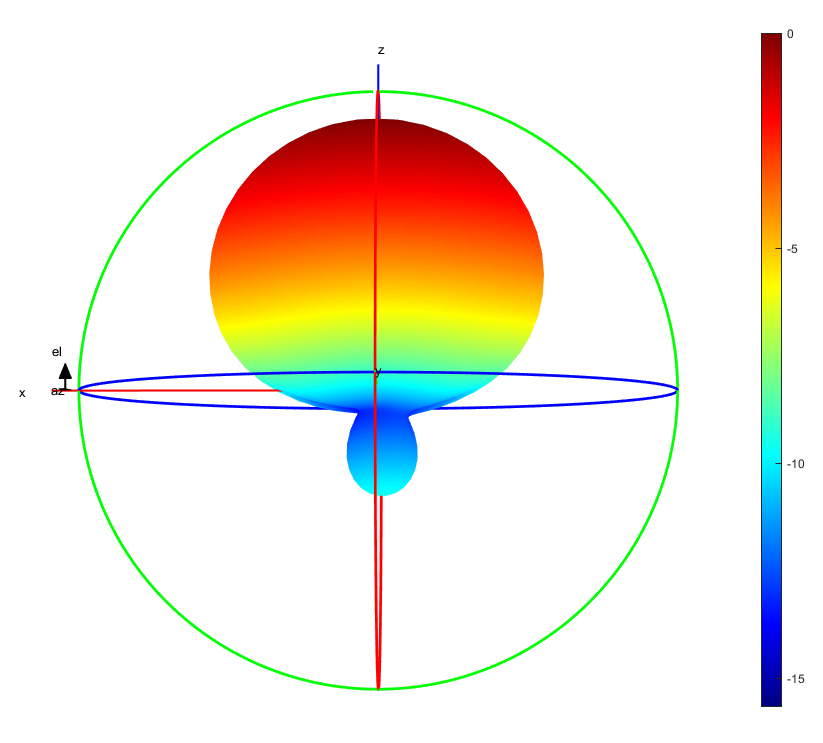
\includegraphics[width=\linewidth]{../images/pattern2/pattern.png}
\endminipage\hfill
\minipage{0.32\textwidth}
  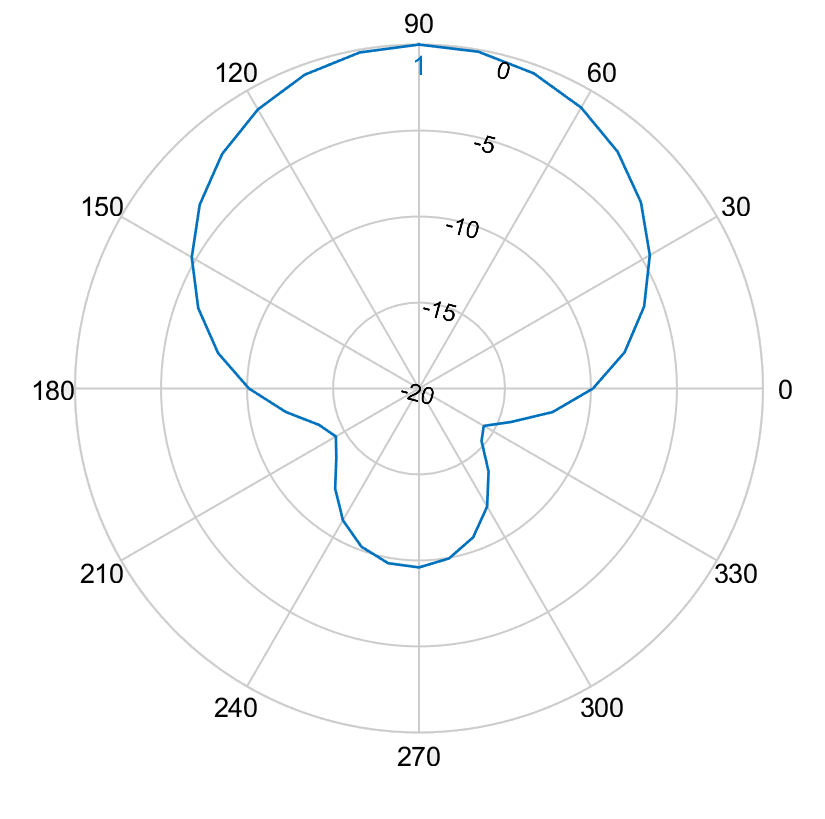
\includegraphics[width=\linewidth]{../images/pattern2/ep.png} 
\endminipage\hfill
\minipage{0.32\textwidth}%
  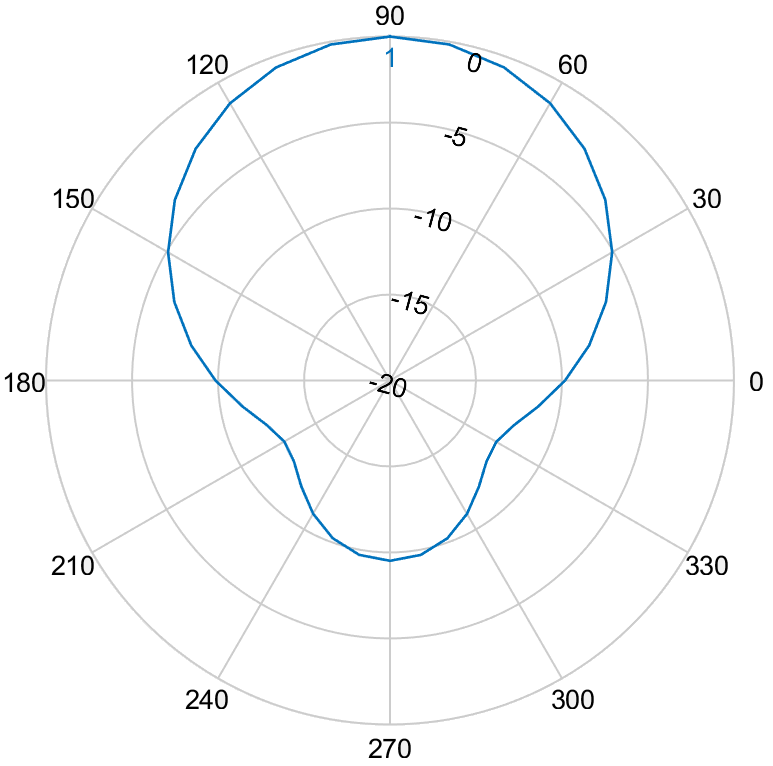
\includegraphics[width=\linewidth]{../images/pattern2/hp.png}
\endminipage
  \caption{Radiation pattern 1: 3D model of the entire pattern on the left with the configuration as described above. In the middle a 2D radiation pattern of the E-plane and at the right a 2D model of the H-plane.}
  \label{radpattern2}
\end{figure}

\begin{figure}[!htb]
\minipage{0.32\textwidth}
  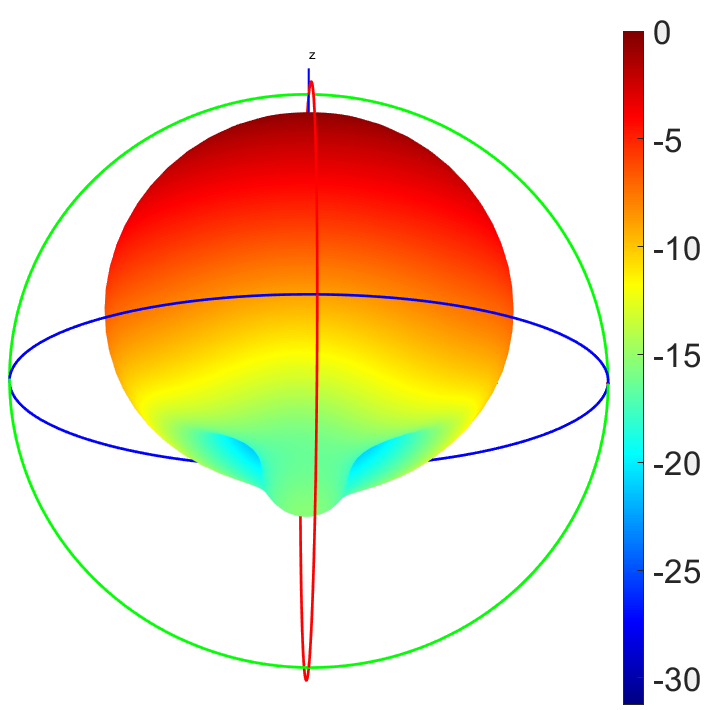
\includegraphics[width=\linewidth]{../images/pattern1/radiationPattern3D.png}
\endminipage\hfill
\minipage{0.32\textwidth}
  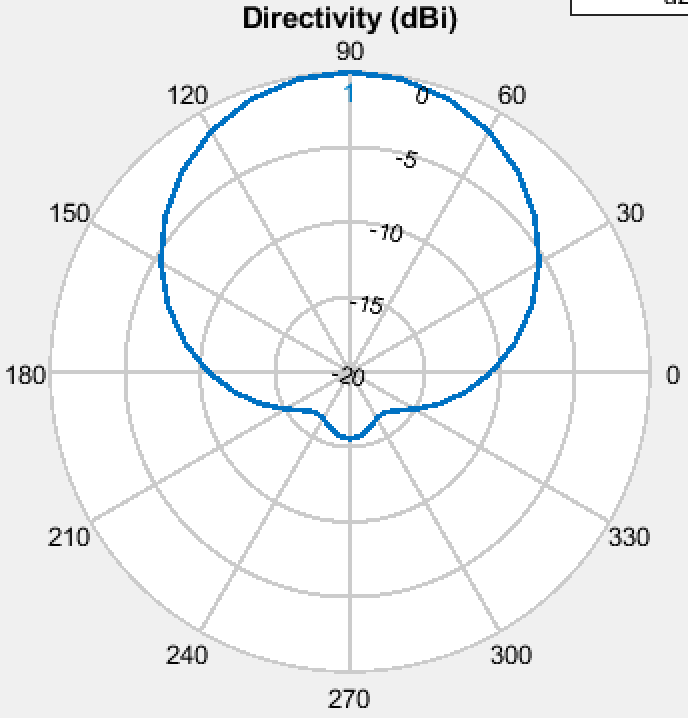
\includegraphics[width=\linewidth]{../images/pattern1/ep.png} 
\endminipage\hfill
\minipage{0.32\textwidth}%
  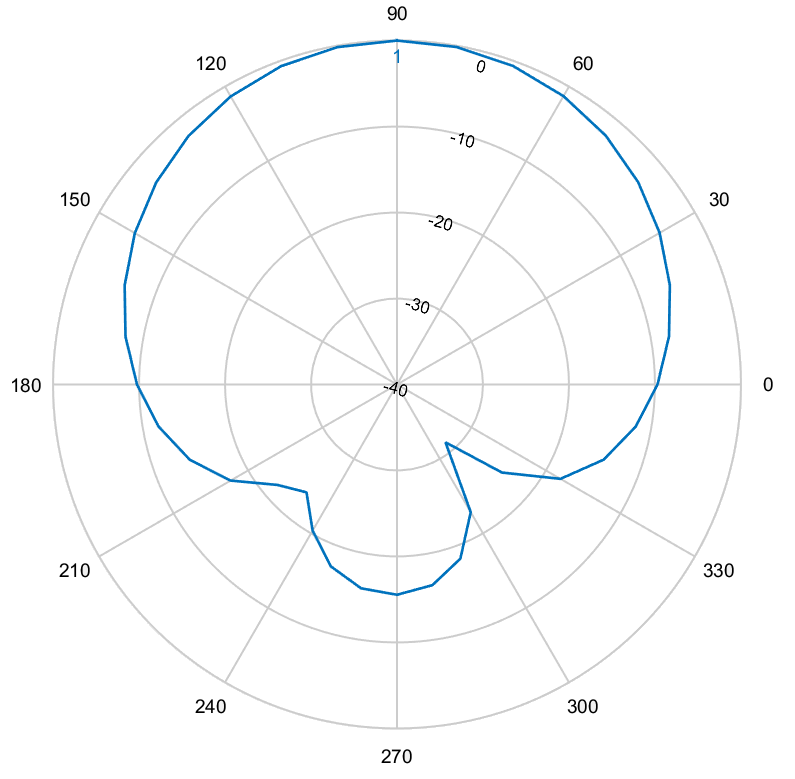
\includegraphics[width=\linewidth]{../images/pattern1/hp.png}
\endminipage
  \caption{Radiation pattern 2: Generated with a groundplane of 0.06m by 0.06m. On the left is the 3D model of the entire pattern plotted. In the middel a 2D radiation pattern of the E-plane and at the right a 2D model of the H-plane.}
 \label{radpattern1}
\end{figure}

\section{Optimizing the network}
The network as originally defined in the deployment tool tried to minimize power consumption by connecting the user to a base stations which
experienced the lowest path loss. A second optimization strategy is introduced, based on the fitness function described in \cite{J1}.

\begin{equation} 
f = w * \left(1 - \frac{E_m}{E_{max}}\right) + (1 - w)*\left(1 - \frac{P}{P_{max}}\right) * 100
\label{eq:fitnessfunction}
\end{equation}

Formula \ref{eq:fitnessfunction} returns a fitness value. Users are connected to different \gls{UABS}s and each time the fitness value is 
calculated. The user will eventually be connected to the drone which resulted in the highest fitness value. This process is repeated for each user.
$w$ is the importance factor of electromagnetic exposure ranging from 0 to 1 with boundaries included. A $w$ set to zero means that electromagnetic 
exposure is not important. Such a network will therefore be called a power consumption optimized network. 
Likewise, a $w$ set to one means that minimizing exposurer is top priority and will result in an exposure optimized 
network. $P_{max}$ is the power consumption of all \gls{UABS}s, both active and non active, when radiating at the highest possible level 
while $P$ is the effective used power by the current designed network. 
This will be the power required for the flying drones themselves and their antenna.
$E_m$ will be the weighted exposure of the average user for the current designed network and $E_{max}$ the electromagnetic exposure when all antennae are at their highest power level.

When optimizing the network, it is not only important to consider the mean exposure of all users but also limit high extrema  \cite{J1}. A weighted average 
will be  used not only considering the median but also the  95 percentile from all users their \gls{DL} exposure using formula \ref{eq:em}. 
Since both values are considered to have equal importance, the weighing factors $w_1$ and $w_2$ will both have an equal importance of 50 \%. 

\begin{equation} 
E_m = \frac{w_1 * E_{50} + w_2 * E_{95}}{w_1 + w_2}
\label{eq:em}
\end{equation}
\textcolor{red}{todo: in J1 is dit gedetailleerder uitgeschreven. Mogelijk om hier wat extra over te schrijven.}


\section{Implementation}

\subsection{Network planning}
\textcolor{red}{todo: Thereafter, all inactive users are deleted and only the x best bs are kept with x equal to facilityCapacity. Eventually, exposure is one last time calculated and objects are initialized with the correct exposure values.}

\subsection{Implementation of the radiation pattern}
\label{subsec:implementationradpat}
The deployment tool originally only supported \gls{isotropicradiator}'s. The tool has thus been extended and is fully configurable allowing any possible antenna 
in any possible 
orientation with the usage of a XML-file. The configuration described in this file will apply to all \gls{UABS}s. 

The orientation is done using two values called `downtilt' and `north offset'. The first value
defines the downtilt angle under wich the antenna is pointing. An downtilt angle of zero degrees is perfectly horizontal and 
an antenna with a downtilt angle of \ang{90} will be pointing straight to the ground.
This parameter only supports positive values ranging from \ang{0} to \ang{360} (upper boundary not included). An antenna pointing to the sky would therefore require a value of \ang{270}.
The second value, the north offset, defines the azimuth orientation of the drone. The value given to this parameter indicates the offset between the north
and the horizontal direction to which the antenna should be pointing to. The value once again ranges from \ang{0} to \ang{360} with the upper boundary not included. The
angle is calculated in counter clock wise orientation. For instance, a north offset of \ang{270} will let the \gls{UABS} point to the east.  

Thereafter, the normalized radiation pattern is supplied to the tool. The actual pattern is three dimensional. To simplify this,
slices perpendicular to the az-axis are extracted. These are indicated at figure \ref{fig:slicesOfPattern} with azimuth cuts. With
an angle of \ang{90}, four slices are achieved, each consisting out of elevation cuts. The intersection of an elevation and azimuth plane 
corresponds with a certain attenuation which is fed to the tool. Figure \ref{fig:slicesOfPattern} show only 3 elevation planes. The radiation pattern used in the tool 
has an attenuation every \ang{10}. In other words, a slice consist of 19 values ranging from \ang{0} to \ang{180} (boundaries included).

\begin{figure}[H]
  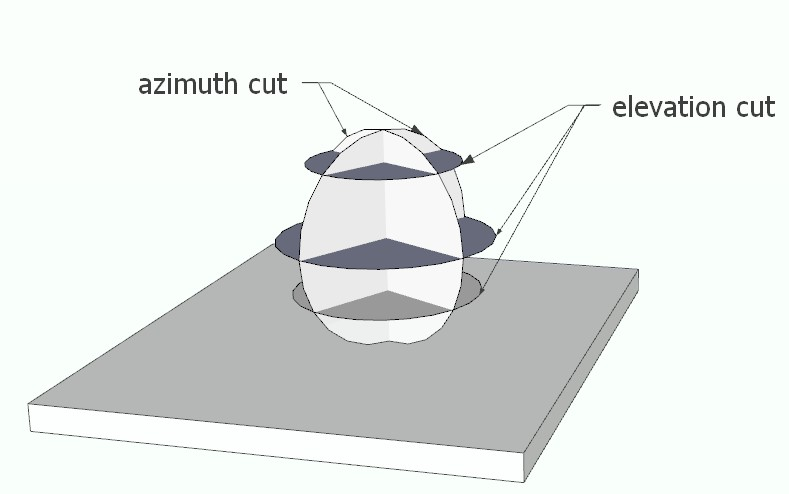
\includegraphics[width=\textwidth]{../images/3Dimages/slicesOfPattern.jpg}
  \caption{Schematic example of slices in a radiation pattern.}
  \label{fig:slicesOfPattern}
\end{figure}

The number of required sliced depend on the complexity of the radiation pattern. For symmetrical radiation patterns like 
in figure \ref{radpattern2} and  \ref{radpattern1}, two azimuth cuts perpendicular to each other dividing the radiation pattern in 4 azimuth-slices 
is definitely sufficient. However, this might not be the case for radiation patterns with a more complex structure containing several  
side lobs. To tackle this issue, more azimuth-slices can be defined for increased precision. Each slice should however contain an equal amount 
of elevation slices.  A concrete example of a configuration file can be found in appendix \ref{ch:radpatexampleconfig}.

When the attenuation of a user from a certain \gls{UABS} needs to be known, the elevation and azimuth angles between the user and the antenna's direction 
should be calculated. 
Figure \ref{fig:globe} represents a radiation pattern with the black dot indicating the user for which the attenuation needs to be calculated.
 The small black lines represent azimuth and elevation planes. 
The tool knows the exact attenuation only at the intersection of those lines. 
The change that the user is positioned at such an intersection is very small. Therefore, the attenuation for the requested point has be estimated using bilinear interpolation.
First, the attenuation is estimated for the intersection of the red-orange line using linear interpolation on the horizontal axis using the known values
 at the end of the red line. The same is done for the orange-green intersection using the known values at the end of the green line. Finally, linear interpolation
is applied to the y-axis for the black dot on the orange line using the estimated values at the end of the orange line.

\begin{figure}[H]
\centering
  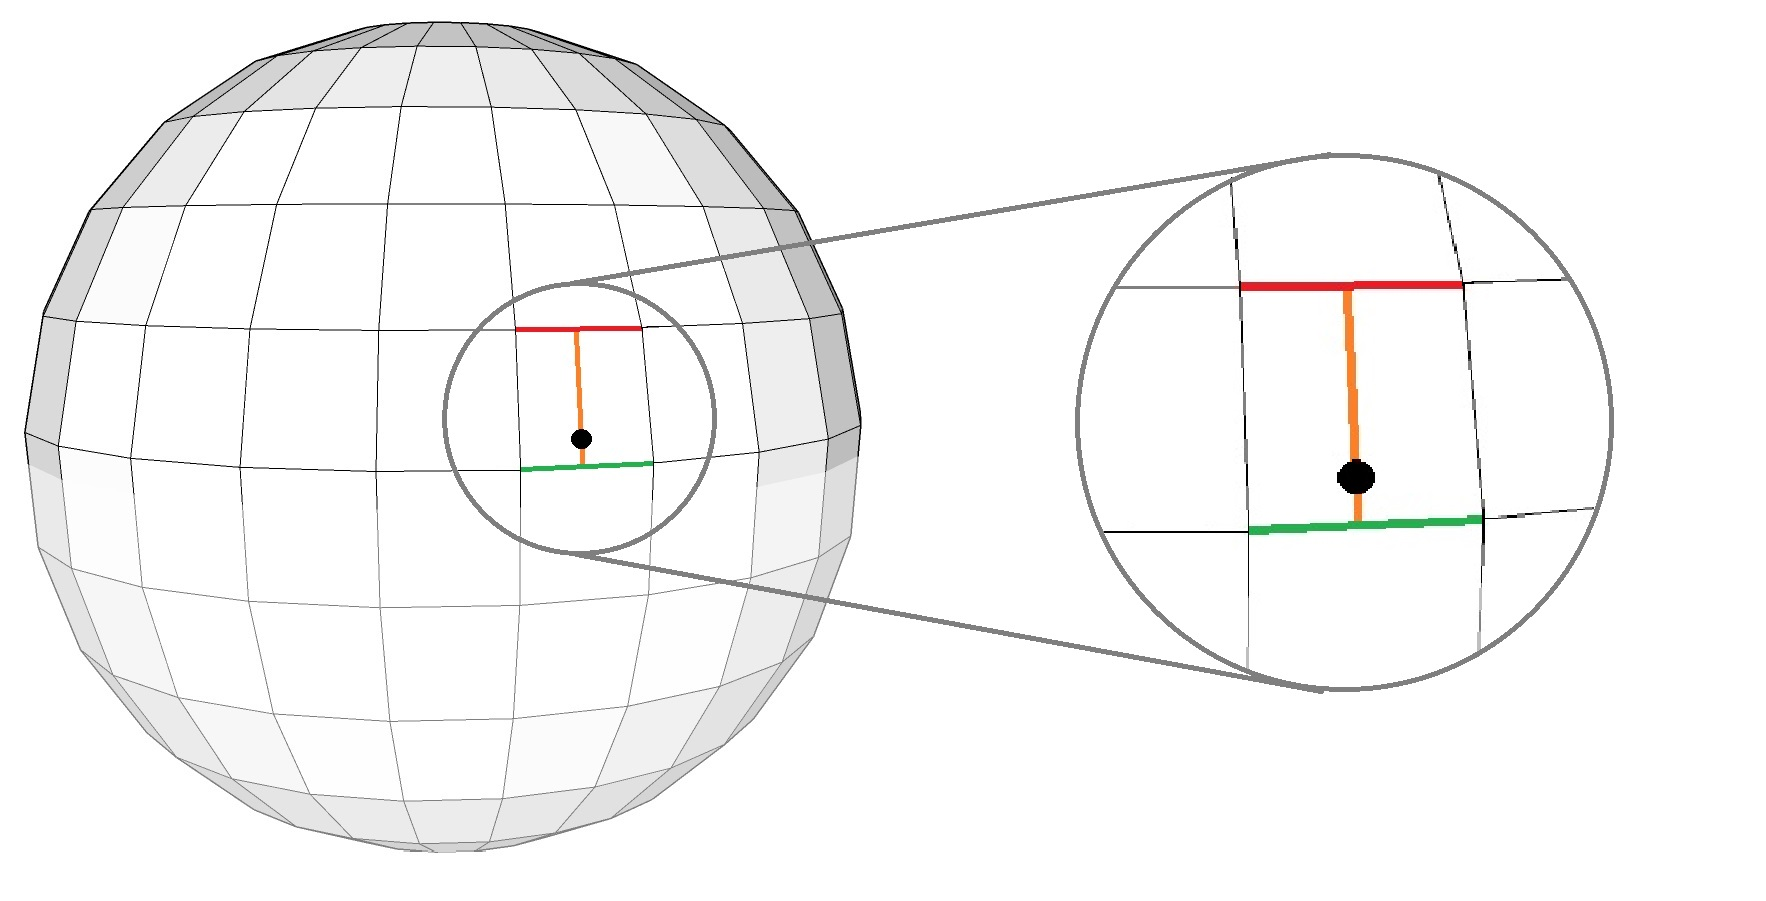
\includegraphics[width=\textwidth/3*2]{../images/3Dimages/globev2.jpg}
  \caption{Schematic example of how bilinear interpollation works.}
  \label{fig:globe}
\end{figure}

\subsection{Performance improvement}
\subsubsection{Calculating path loss}
The path loss is required for several formulas. For instance, each user decides whether a \gls{UABS} is feasible based 
the path loss but also the calculations for the downlink electromagnetic 
exposure require this value to be known. The formulas for the whole body $SAR_{10g}$ require not only the path loss between the user
and all \gls{UABS}s but even the path loss between users themselves. These path loss calculations are based and the Walfisch-Ikegami 
model that causes a high computational load. The calculation between two points stands completely free from
any other calculation between any other point and is therefore a suitable candidate to be multithreaded. The deployment tool creates two thread pools.
The first pool creates a thread for each user where each thread calculates the path loss between the user assigned to him and all possible \gls{UABS}s,
 causing a time complexity of $n^2$.
Each user stores all path losses between himself and any other \gls{UABS} and result therefore in a total space complexity of $n^2$.
When all users are finished, the thread pool is shut down and the second one is created for the same calculations but between users.
The pool will, just like the previous, create threads for each user but has an important difference.
When a certain user calculates the path loss to another user, this path loss also applies for the other direction. The tool saves time by calculating the path loss only 
once and stores the path loss by both users. It is therefore sufficient that a given user only calculates path losses to users right of him, since the other will 
be calculated by the users left to him. This results in a time complexity of only $n(\frac{n}{2})$. When the last user finishes his thread, all users know the path loss to all other users causing 
a space complexity of $n(n-1)$.
% eventueel nog over concurrent hashmap

\subsubsection{Limiting antenna searching}
The user needs to be connected to the `best' base station. To identify this best \gls{UABS}, the user should be connected 
to each base station and the fitness value \ref{eq:fitnessfunction} of the network should be evaluated. The connection that resulted in the best fitness function
will be added to the solution. This process is repeated for each user but can further be improved. A user will likely be connected to either 
\gls{UABS} directly above him or to a \gls{UABS} in the direct neighborhood. Time complexity can thus be improved by not considering drones 
outside a certain radius.
An ideal data structure for neighborhood-search is a KD-tree. This data structure is based on a binary tree and optimal for objects with 
multiple keys. Objects are thus positioned in K dimensions where each node split the hyperplane over exact one dimension. The dimension that need 
to be split depends on the level of the KD-tree where that node is situated.
In this case, the x and y coordinate will be used in a 2D-tree (k=2) like in figure \ref{fig:exampleKDtree}.

\begin{figure}[H]
  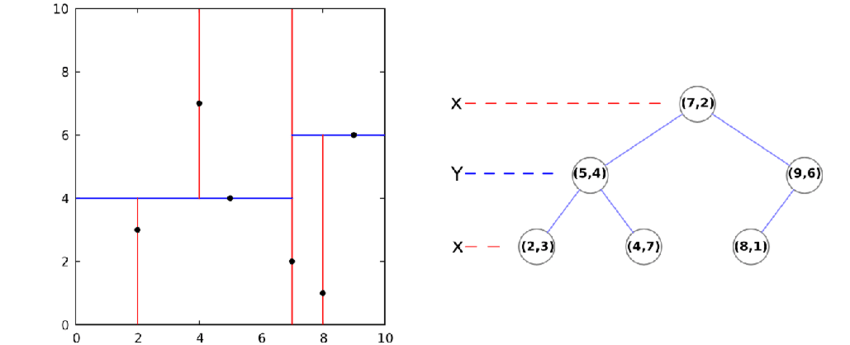
\includegraphics[width=\textwidth]{../images/Example-of-a-2D-k-d-tree.png}
  \caption{Example of a KD-three in two dimensions}
  \label{fig:exampleKDtree}
\end{figure}
\textcolor{red}{TODO: schrijf ook voor 200 users.Here, is chosen to consider only \gls{UABS}s within a radius of half a kilometer. In a scenario of 500 \gls{UABS}s, 60 possible \gls{UABS}s are verified.}
%\chapter{Implementation}
\label{chap:implementation}

\section{Implementation of downlink exposure}
\label{sec:downlinkimplementation}

Schrijf over hoe die exposure nu toegevoegd is aan de tool. 
-Wat deed de tool al? Users en femtocell's uniform verdelen op publiek transport, uabs etc
- dat de exposure pas op het einde wordt berekend nadat het netwerk gemodeleerd is.

Algorithm \ref{alg:getexposure} describes the implementation on how to calculate the exposure of a user towards a single base station as described in formula \ref{eq:singleexposure}.
Several values need to be known for this to work. In the first place, the path loss is calculated.  However, the different path loss values are already calculated during the network initialization phase and can, therefore, be reused on the condition they were saved. By only calculating the path loss once,  the time complexity of the tool decreases drastically. 
Afther this, the gain is calculated by adding the antenna gain to the  current input power of the antenna and by substracting the feeder loss as already stated in equation \ref{eq:eirp}.
In the last place, equation \ref{eq:singleexposure} is used and the exposure is returned.

\begin{algorithm}
	\caption{getExposure} 
	\label{alg:getexposure}
     \hspace*{\algorithmicindent} \textbf{Input} user, basestation\\
     \hspace*{\algorithmicindent} \textbf{Output} exposure of a user towards a single basestation
	\begin{algorithmic}[1]
        \State $PL \gets$ path loss between user and basestation
        \State $gain \gets$ getBSantennagain + basestation.getInputPower - getBSFeederLoss
		\State $exposure \gets 10^{\frac{EIRP - 43.15 + 20*\log(f)- PL}{20}}$ \\
    \Return $exposure$ 
	\end{algorithmic} 
\end{algorithm}

To combine all exposures for a specific user, equation \ref{eq:totalexposure} is translated into algortim \ref{alg:gettotalexposure}.
Finaly, this needs to be repeaded for every users. Algorithm \ref{alg:main} is used to iterate over each user and each simulation and saves the computed value
into the appropriate attribute.

\begin{algorithm}
	\caption{getTotalExposure} 
	\label{alg:gettotalexposure}
     \hspace*{\algorithmicindent} \textbf{Input} user, basestations[]\\
     \hspace*{\algorithmicindent} \textbf{Output} combined exposures from each basestation for a given user
	\begin{algorithmic}[1]
        \State $E_{tot}\gets 0.0$
		\ForAll {basestation  in  basestations}
            \State $E \gets$ getExposure(user, basestation)
            \State $E_{tot}\gets E_{tot} + E^2$	
		\EndFor
        \State $E_{tot}\gets sqrt(E_{tot})$\\
    \Return $E_{tot}$ 
	\end{algorithmic} 
\end{algorithm}

\begin{algorithm}
	\caption{Calculate and save the total exposure for each user in each simulation} 
	\label{alg:main}
     \hspace*{\algorithmicindent} \textbf{Input} users[][], basestations[][]\\
     \hspace*{\algorithmicindent} \textbf{Output} /
	\begin{algorithmic}[1]
		\For {$simulation=1,2,\ldots basestations$}
			\ForAll {user  in  users[simulation]}
				\State $user.exposure \gets  getTotalExposure(user,basestations[simulation])$
			\EndFor
		\EndFor
	\end{algorithmic} 
\end{algorithm}

To provide a summary of how the network is performing on electromagnetic exposure, a weighted average is calculated. This is implemented in algorithm \ref{alg:getglobaluserexposure} which
takes all users for a specified simulation and two weighting factors $w_1$ and $w_2$. They respectively correspond to the 50th percentile and 95th of the ordered users' exposure. The two weights get equal importance of 0.5. This is because also higher values should be taken into account and not compensated with very low values. The formula will only use electric field strengths where users are active as opposed to \cite{J1} where the area is divided into grids and the exposure is calculated for every gridpoint. The reasoning behind this is that the goal of this master dissertation is to calculate the average exposure of the user and not of the entire area.

The formula first calculates the index where the mean value and the 95th percentile should be located. Afterwards, the exposure is calculated using interpolation if necessary.

\begin{algorithm}
	\caption{globalUserExpsoure} 
	\label{alg:getglobaluserexposure}
     \hspace*{\algorithmicindent} \textbf{Input} users[], $w_1$, $w_2$\\
     \hspace*{\algorithmicindent} \textbf{Output} Weighted average of the median  and the $95th$ percentile electric field strenght
	\begin{algorithmic}[1]
		\State Sort users by $E_{tot}$
		
 		\Comment{E50}
		\State $meanIndex \gets \frac{users.length}{2}$
		\If{users.length \% 2 == 0}
			\State $E_{50} \gets users[meanIndex].exposure$ 
		\Else
			\State $E_{50} \gets \frac{(users[ \left \lceil{meanIndex}\right \rceil ].exposure) + (users[ \left \lfloor{meanIndex}\right \rfloor ].exposure)}{2}$ 
		\EndIf

		\Comment{E95 with interpolation}
		\State $ X \gets users.length * 0.95$ 
		\State $ X_1 \gets \left \lfloor{x}\right \rfloor $ 
		\State $ X_2 \gets \left \lceil{x}\right \rceil $ 
		\State $ Y_1 \gets users[X_1].exposure$ 
		\State $ Y_2 \gets users[X_2].exposure$ 
		\State $E_{95} \gets  Y_1 + \left(\frac{(X - X_1)}{(X_2 - X_1)}* (Y_2 - Y_1)\right)$\\
		\Return $\frac{(w_1* E_{50})+ (w_2 * E_{95})}{w_1 + w_2}$
	\end{algorithmic} 
\end{algorithm}

%%%%%%%%%%%%%%%%%%%%%%%%% SECTIOIN %%%%%%%%%%%%%%%%%%%%%%%%
\section{Implementation of uplink exposure}
\label{sec:uplinkexposure}

Analogously to the \ref{sec:downlinkimplementation}, the uplink calculator will determine the uplink exposure and save in the appropriate user object. The calculator starts with iterating over each user in each simulation and calls the getSar() function.

\ref{eq:sar10g} is implemented in \ref{algo:getsar}. The function requires a user as input for which the uplink exposure should be calculated and two constant values which should be declared once. The maximal allowed $SAR_{10g}$ as discussed in \ref{sec:sar} and maximal permitted transmission power of 23 dbm.

Also, the actual transmitting power of the \gls{UE} needs to be calculated using the getActualTransmitPower function. 

Both $Tx_{watt}$ and $TX^{max}_{watt}$ are converted to watt. This is because the decibel variant can range from -57 dBm to 23 dBm \cite{J10_RDPgit}. Converting to Watt results in a solely positive fraction. 

After having multiplied with the maximum allowable \gls{SAR}, the actual uplink exposure is returned.

\begin{algorithm}
	\caption{getSar} 
	\label{alg:getsar}
     \hspace*{\algorithmicindent} \textbf{Input} user \\
     \hspace*{\algorithmicindent} \textbf{Output} $SAR_{10g}$
	\begin{algorithmic}[1]
		\State  const $SAR^{max} \gets 0.67$
		\State  const $TX^{max}_{watt} \gets dBm2W(23)$
		\vspace{4 mm}
		\State $Tx_{watt} \gets dBm2W(getActualTransmitPower(user)) $		
		\State $ SAR_{10g} \gets \frac{Tx_{watt}}{TX^{max}_{watt}} * SAR^{max}$ \\
		\Return $ SAR_{10g}$
	\end{algorithmic} 
\end{algorithm}


The implementation for getActualTransmitPower is described in \ref{alg:getActualTransmitPower}. This function requires a user as a parameter and will calculate the real used power for transmission in dBm.
Once again, a global constant value is defined describing the maximum allowable transmitting power $Tx^{max}_{dBm}$ expressed in dBm. The predicted transmitting power is achieved by subtracting the path loss between the user and the affective femtocell with the receiver sensitivity of the femtocell. However, this value can't be higher then  $Tx^{max}_{dBm}$ , if this is the case the maximum allowable transmitting power is returned instead.

\begin{algorithm}
	\caption{getActualTransmitPower} 
	\label{alg:getActualTransmitPowergit}
     \hspace*{\algorithmicindent} \textbf{Input} user \\
     \hspace*{\algorithmicindent} \textbf{Output} The actual used power for transmition in dBm.
	\begin{algorithmic}[1]
		\State const $Tx^{max}_{dBm} \gets 23$
		\vspace{4 mm}
		\State $ Tx_{dBm} \gets user.getPathLoss() - technology.getFemtocellReceiverSensitivity(user.getRxSNR)$ \\
		\Return $min(Tx_{dBm}, Tx^{max}_{dBm})$ 
	\end{algorithmic} 
\end{algorithm}


%\begin{algorithm}
%	\caption{getFemtocellReceiverSensitivity} 
%	\label{alg:getFemtocellReceiverSensitivity}
%     \hspace*{\algorithmicindent} \textbf{Input} user \\
%     \hspace*{\algorithmicindent} \textbf{Output} The receiver sensitivity of the femtocell in dBm
%	\begin{algorithmic}[1]
%		\State $SNR \gets user.getRxSNR$
%		\State $gain \gets technology.getMSantennagain$
%		\State $implementationLoss \gets technology.getImplementationLoss$
%		\State $interferenceMargin \gets technology.getCellInterferenceMargin$
%		\State $noiseFigure \gets technology.getNoiseFigure$
%		\State $thermalNoise \gets -108.1$	\\
%		\Return  $thermalNoise + SNR - gain + implementationLoss + noiseFigure + interferenceMargin$
%	\end{algorithmic} 
%\end{algorithm}


\chapter{Results and Discussion}
\label{chap:results}

This chapter gives an overview of the achieved results from all considered scenarios and cases.
The first section talks about a small network with only one user and one \gls{UAV}s. In 
the following section, this network is expanded for a larger population but still with one \gls{UAV}s.
The last section is also for a large population but with an unlimited number of \gls{UAV}s.

%%%%%%%%%%%%%%%%%%%%%%%%%%%%%%%%%%%%%%%%%%%%%%%%%%%%%%%%%%%%%%%%%%%%%%%%%%%%%%%%%%%%%%%%%%%%%%%%%%%%%%%%%%%%%%%%%%%%%%%%%%%%%%%%%%%%
\section{Scenario 1: One User and One \gls{UAV}}
The network contains only one user in this scenario. This means that there is only one location possible for the \gls{UAV} which will 
be just above 
the user. This section will investigate minimal required transmission power and SAR values from different sources.
Finally, also the power consumption of the entire network is measured. The  ``entire network" refers to all \gls{UABS}s. The entire network 
will for the first scenario be constructed out of a singe \gls{UABS}.

\subsection{The Influence of the Maximum Transmission Power}
\label{s1a}
\gls{LTE} makes usage of power control meaning that no more power will be used than strictly necessary. The actual 
transmission power $P_{tx}$ therefore ranges between zero and the maximum allowed input power. $P_{tx}$ is zero when the \gls{UABS} doesn't cover anybody.
For instance when the flying height is too high and therefore also the path loss that comes with it, the maximum allowed $P_{tx}$ is not enough to cover 
the distance. In such case, the \gls{UABS} is shut down since it cannot meet the requirements.
Increasing the maximum transmission power will not influence the actual used $P_{tx}$ or $SAR_{10g}$ because the \gls{UABS} will not use more
than strictly required. It is therefore more useful to match the actual transmission power against a variable flying height. 

Figure \ref{fig:ptxfh} shows a logarithmic relationship between $P_{tx}$ and flying height.
As already discussed in \ref{sec:scenarios_s1}, the user is outdoor and just below the \gls{UABS}. There is thus a free line-of-sight between both
radiators. It is clear from figure \ref{fig:ptxfh} that a discontinue step function is achieved. This is because multiple flying heights correspond to the same transmission power.
When the flying height increases, so does the path loss. \gls{LTE} tries to counteract this by increasing the power level. Each time 
the path loss becomes too high, the power level of the antenna increases with one dBm. Doing so, decreases path loss allowing the antenna to reach
the user again. 

\begin{figure}[t]
  \centering
  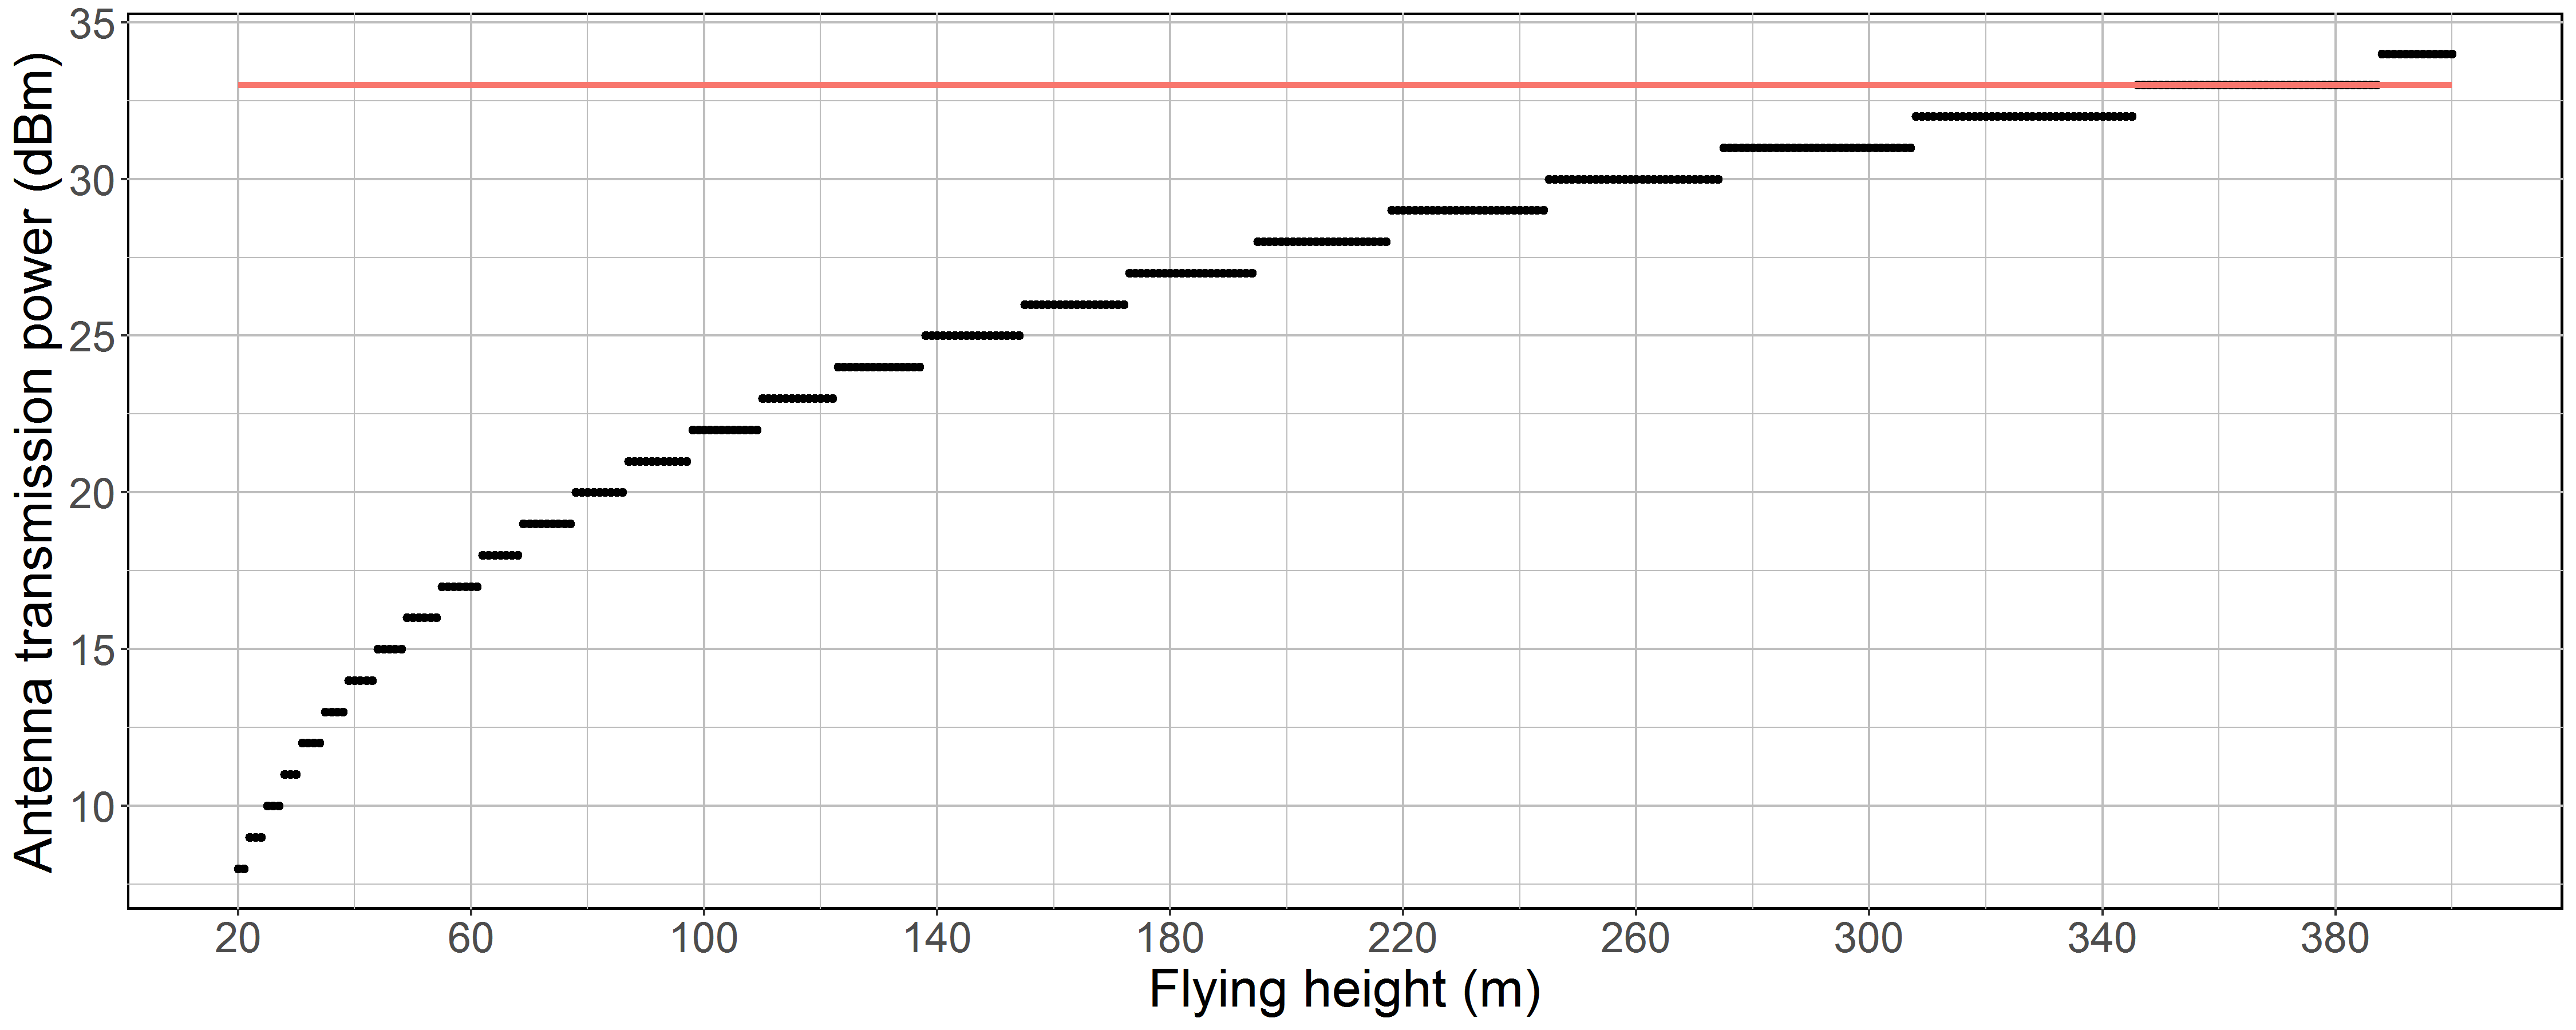
\includegraphics[width=\textwidth]{../results/s1/ptx.png}
  \caption{Minimal required transmission power by the antenna to reach the ground just below him. The red line shows the default maximum transmission power.}
  \label{fig:ptxfh}
\end{figure}

After a jump in the step function, there is an overestimation meaning the input power increased more than necessary. So multiple flying heights correspond with the same $P_{tx}$.
Further, dBm is also a logarithmic scale meaning that while 10 dBm equals 10 mW, 20 dBm equals 100 mW. This explains why the black lines become longer at higher flying altitudes.
Each time the power level increases with one dBm, the overestimation becomes larger. If the tool would make usage of a smaller step size, a more continuous 
logarithmic function would be achieved. This would however worsen the time complexity because it would take much more iterations before 
the power level exceeds the path loss. 

The red line in figure \ref{fig:ptxfh} indicates the default maximum transmission power used during simulations as 
defined in table \ref{table:defaultconf}. 
In a free line-of-sight scenario with only one user, a \gls{UABS} can fly up to 387 meters before losing connection.

This scenario is investigated with a microstrip patch antenna using power consumption optimization. 
 However, the chosen optimization strategy doesn't really matter as already explained in  \ref{sec:scenarios_s1}. This is because the decision 
 algorithm decides which user 
needs to be connected to which \gls{UABS}. Since only one \gls{UABS} is available, both optimization strategies will behave identical.
Further, also the used antenna will not make any difference
despite the fact that a microstrip patch antenna has attenuation while an \gls{isotropicradiator} doesn't.
The user is namely positioned in the perfect center of the main beam where there is 
no attenuation experienced in either cases. So the results are applicable for the four possible cases from figure \ref{fig:fourCasesMatrix}.

\FloatBarrier
\subsection{Influence of the Flying Height}
\label{sub:senario1_influenceOfFlyHeight}

This section investigates how the flying height of a \gls{UABS} influences $SAR_{10g}$ and power consumption.
The $SAR_{10g}$, which is actually induced electromagnetic radiation into our user, is represented in figure \ref{fig:s1_fhsar}
and shows that for a low flying \gls{UAV}, \gls{UE} is the main source of electromagnetic radiation.
This changes around 80 meters where the \gls{UL} electromagnetic radiation from the \gls{UE}
exceeds the \gls{DL} radiation in order to still be able to reach the high flying \gls{UABS}s.

\gls{SAR}-values are caused by the transmitted power  $P_{tx}$ of the antenna. The $P_{tx}$ in section \ref{s1a}
showed a discontinue behaviour that sometimes radiates more as strictly necessary. This has thus a direct influence
on the \gls{DL} \gls{SAR}. Hence the same discontinue behaviour. The \gls{DL} \gls{SAR} can be simplified to a perfect constant line.
This constant behaviour can once again be explained with power control. When the \gls{UABS} flies lower, there is less path loss and the \gls{UABS} 
will therefore reduce the $P_{tx}$. This results in formula \ref{eq:exposureBasicFormula} where the electromagnetic exposure is a constant fraction of power and distance.

\begin{equation}
\vec{E} (V/m) = \frac{\Delta U (V) }{\Delta x (m)}
\label{eq:exposureBasicFormula}
\end{equation}

%The SAR values are the result of multiplying the electromagnetic exposure with a constant as explained in equation \ref{eq:DLconvertion}. So both have a linear relationship.

Figure \ref{fig:s1_fhsar} doesn't show radiation from neighbours, because there are none present in this scenario. 
Finally, all these values are added up as explained in formula \ref{eq:overallSARwb} resulting in the total \gls{SAR}
to which our user is exposed which is represented by the black line in \ref{fig:s1_fhsar}.

\begin{figure}[]
  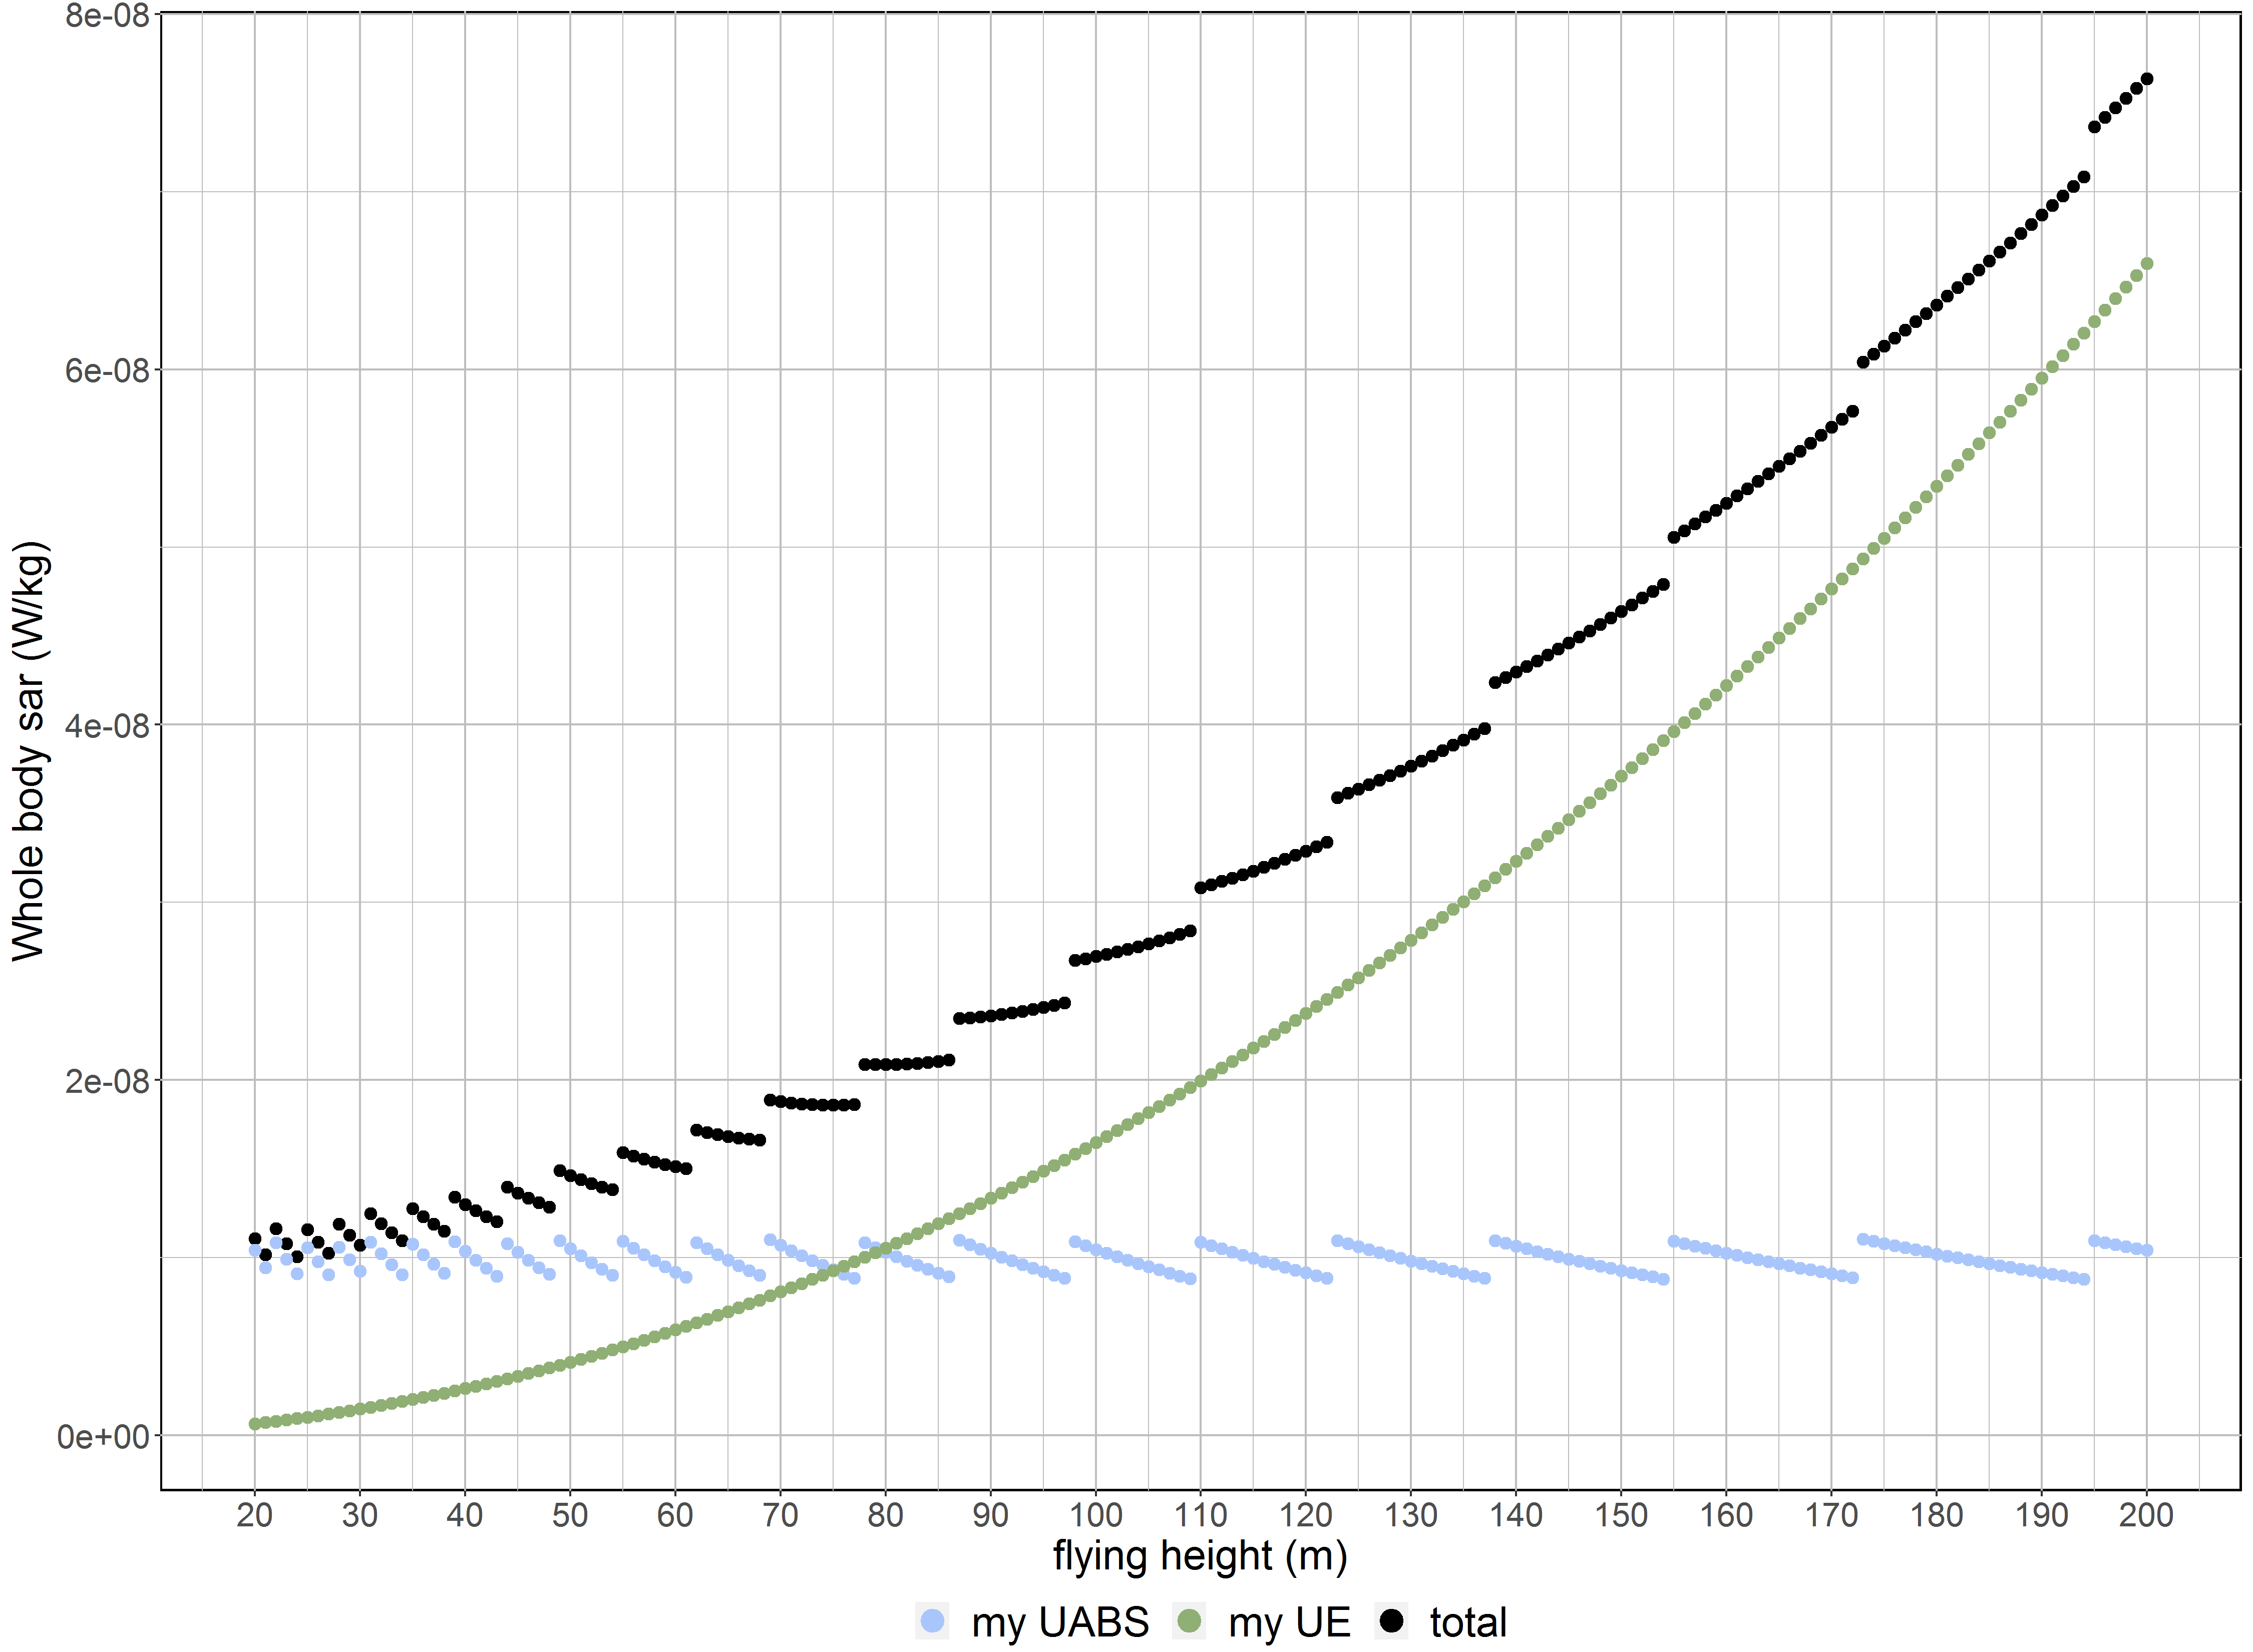
\includegraphics[width=\textwidth]{../results/s1/fhvssar.png}
  \caption{How SAR values from different sources are influenced by different flying altitudes.}
  \label{fig:s1_fhsar}
\end{figure}

The power consumption of the entire network includes both the power required by the \gls{UAV} itself and the antenna he is carrying.
The power consumption of the entire network is here of course for the only \gls{UABS} available. Figure \ref{fig:fhvspc} shows an 
exponential relationship between both power consumption and flying height. 

\begin{figure}[t]
  \centering
  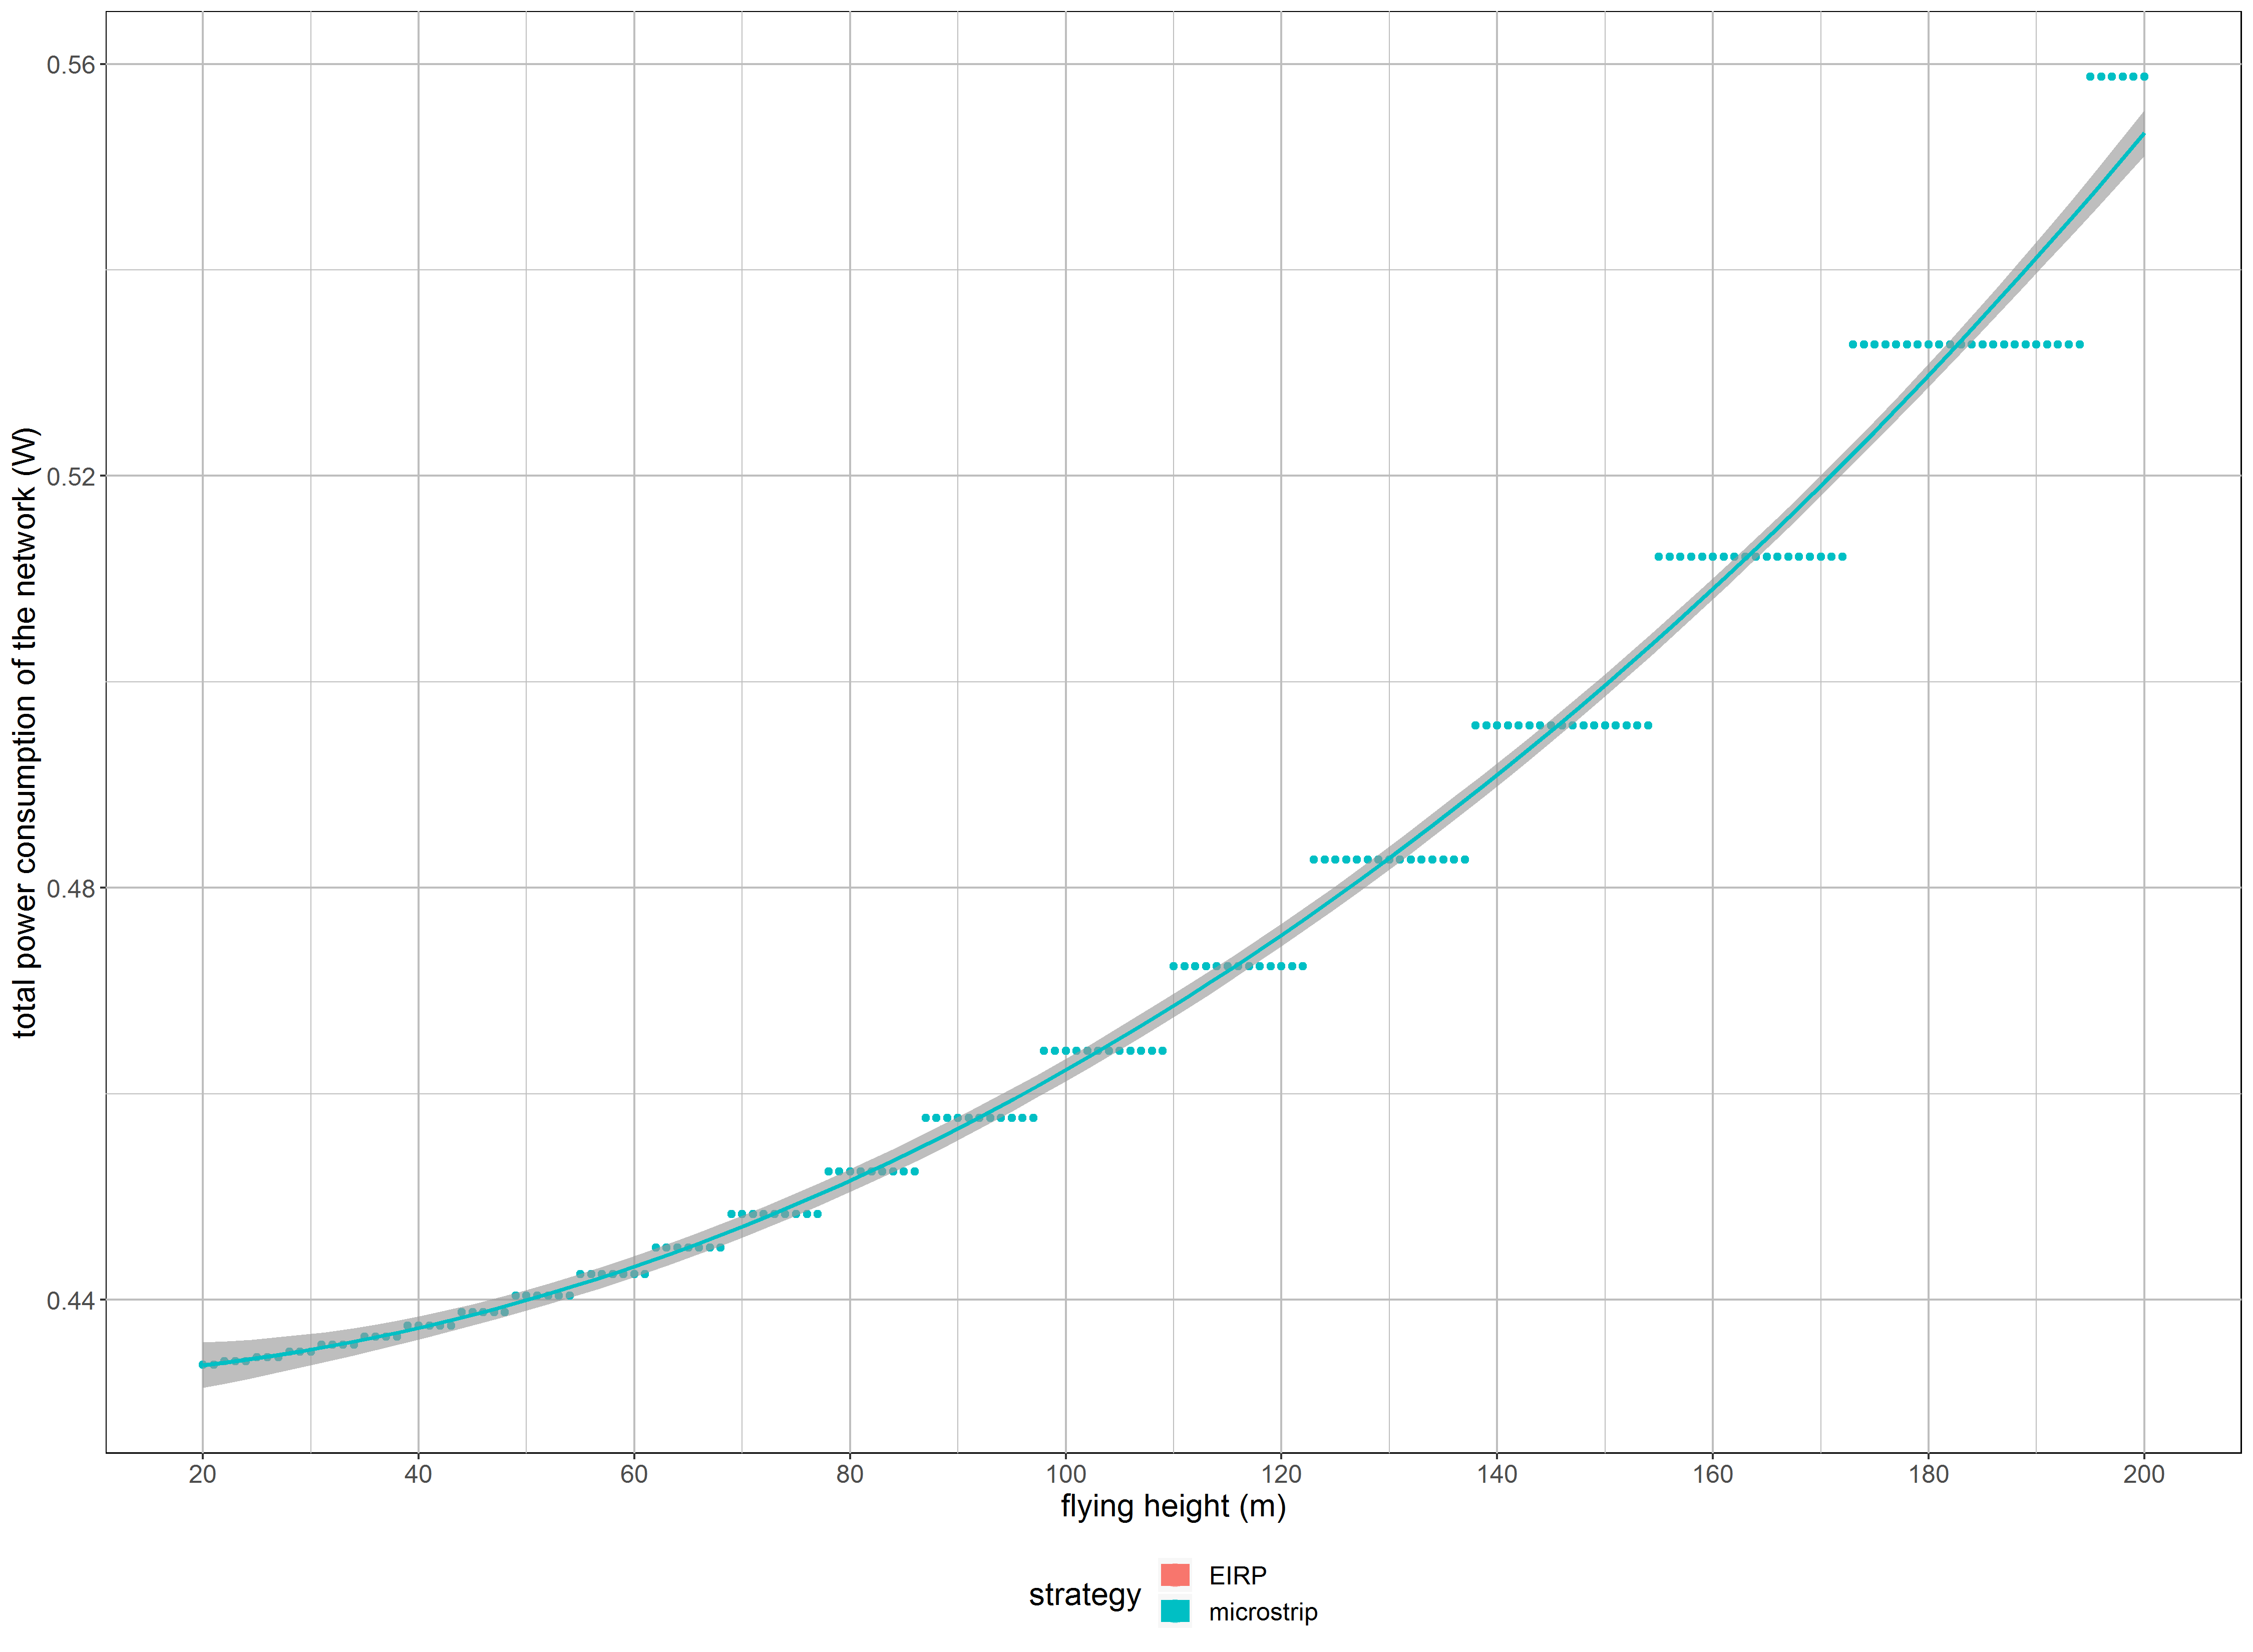
\includegraphics[width=\textwidth]{../results/s1/fhvspc.png}
  \caption{Minimal required transmission power by the antenna to reach the ground just below him. The red line shows the default maximum transmission power.}
  \label{fig:fhvspc}
\end{figure}

%%%%%%%%%%%%%%%%%%%%%%%%%%%%%%%%%%%%%%%%%%%%%%%%%%%%%%%%%%%%%%%%%%%%%%%%%%%%%%%%%%%%%%%%%%%%%%%%%%%%%%%%%%%%%
\FloatBarrier
\section{Scenario 2: Increased Traffic}

This scenario has just like the previous scenario only one \gls{UAV} available. However, more users will be present in the network.
First, a variable flying altitude is investigated for a fixed number of 224 users. 
Secondly, the flying height is set to 100 metres with a variable number of users.
When designing the network, there will be as much possible \gls{UAV} locations as there are users in the network and the tool
will consider all of them. It's only when the programme is finished, that one \gls{UAV} remains.

\subsection{Influence of the Flying Altitude}
The first case investigates how the network, consisting out of one \gls{UABS}, behaves when applied on an ordinary day during rush hour. 
Different fixed flying heights are considered while 224 active users are distributed uniformly over the city center of Ghent. 

A power consumption optimized network with an \gls{EIRP} antenna (green) has the highest exposure. 
This is logical when comparing with an EIRP antenna in an exposure optimized network (red). 
However, when looking at figure \ref{fig:s2a_dlAndPc} on the right, the power consumption in a power consumption optimized network is worse 
than in an exposure optimized network. To understand this, the behaviour of the deployment tool needs to be understood first. 
A power consumption optimized network will result in a few high powered \gls{UABS}s because increasing the input power of an antenna cost 
less then activating a new  \gls{UAV}. Likewise, an exposure optimized network 
generates a lot of low powered \gls{UABS}s because the lower the antenna's power, the lower the exposure. This has the consequence that the cover radius 
is less and therefore requiring more \gls{UAV}s which costs more energy.
When only a limited amount of \gls{UABS}s are available, 
like only one in this scenario, the tool will only keep \gls{UABS}s which cover the most users. 
Therefore is the power consumption in a power consumption optimized network way higher. 


\begin{figure}[h!]
  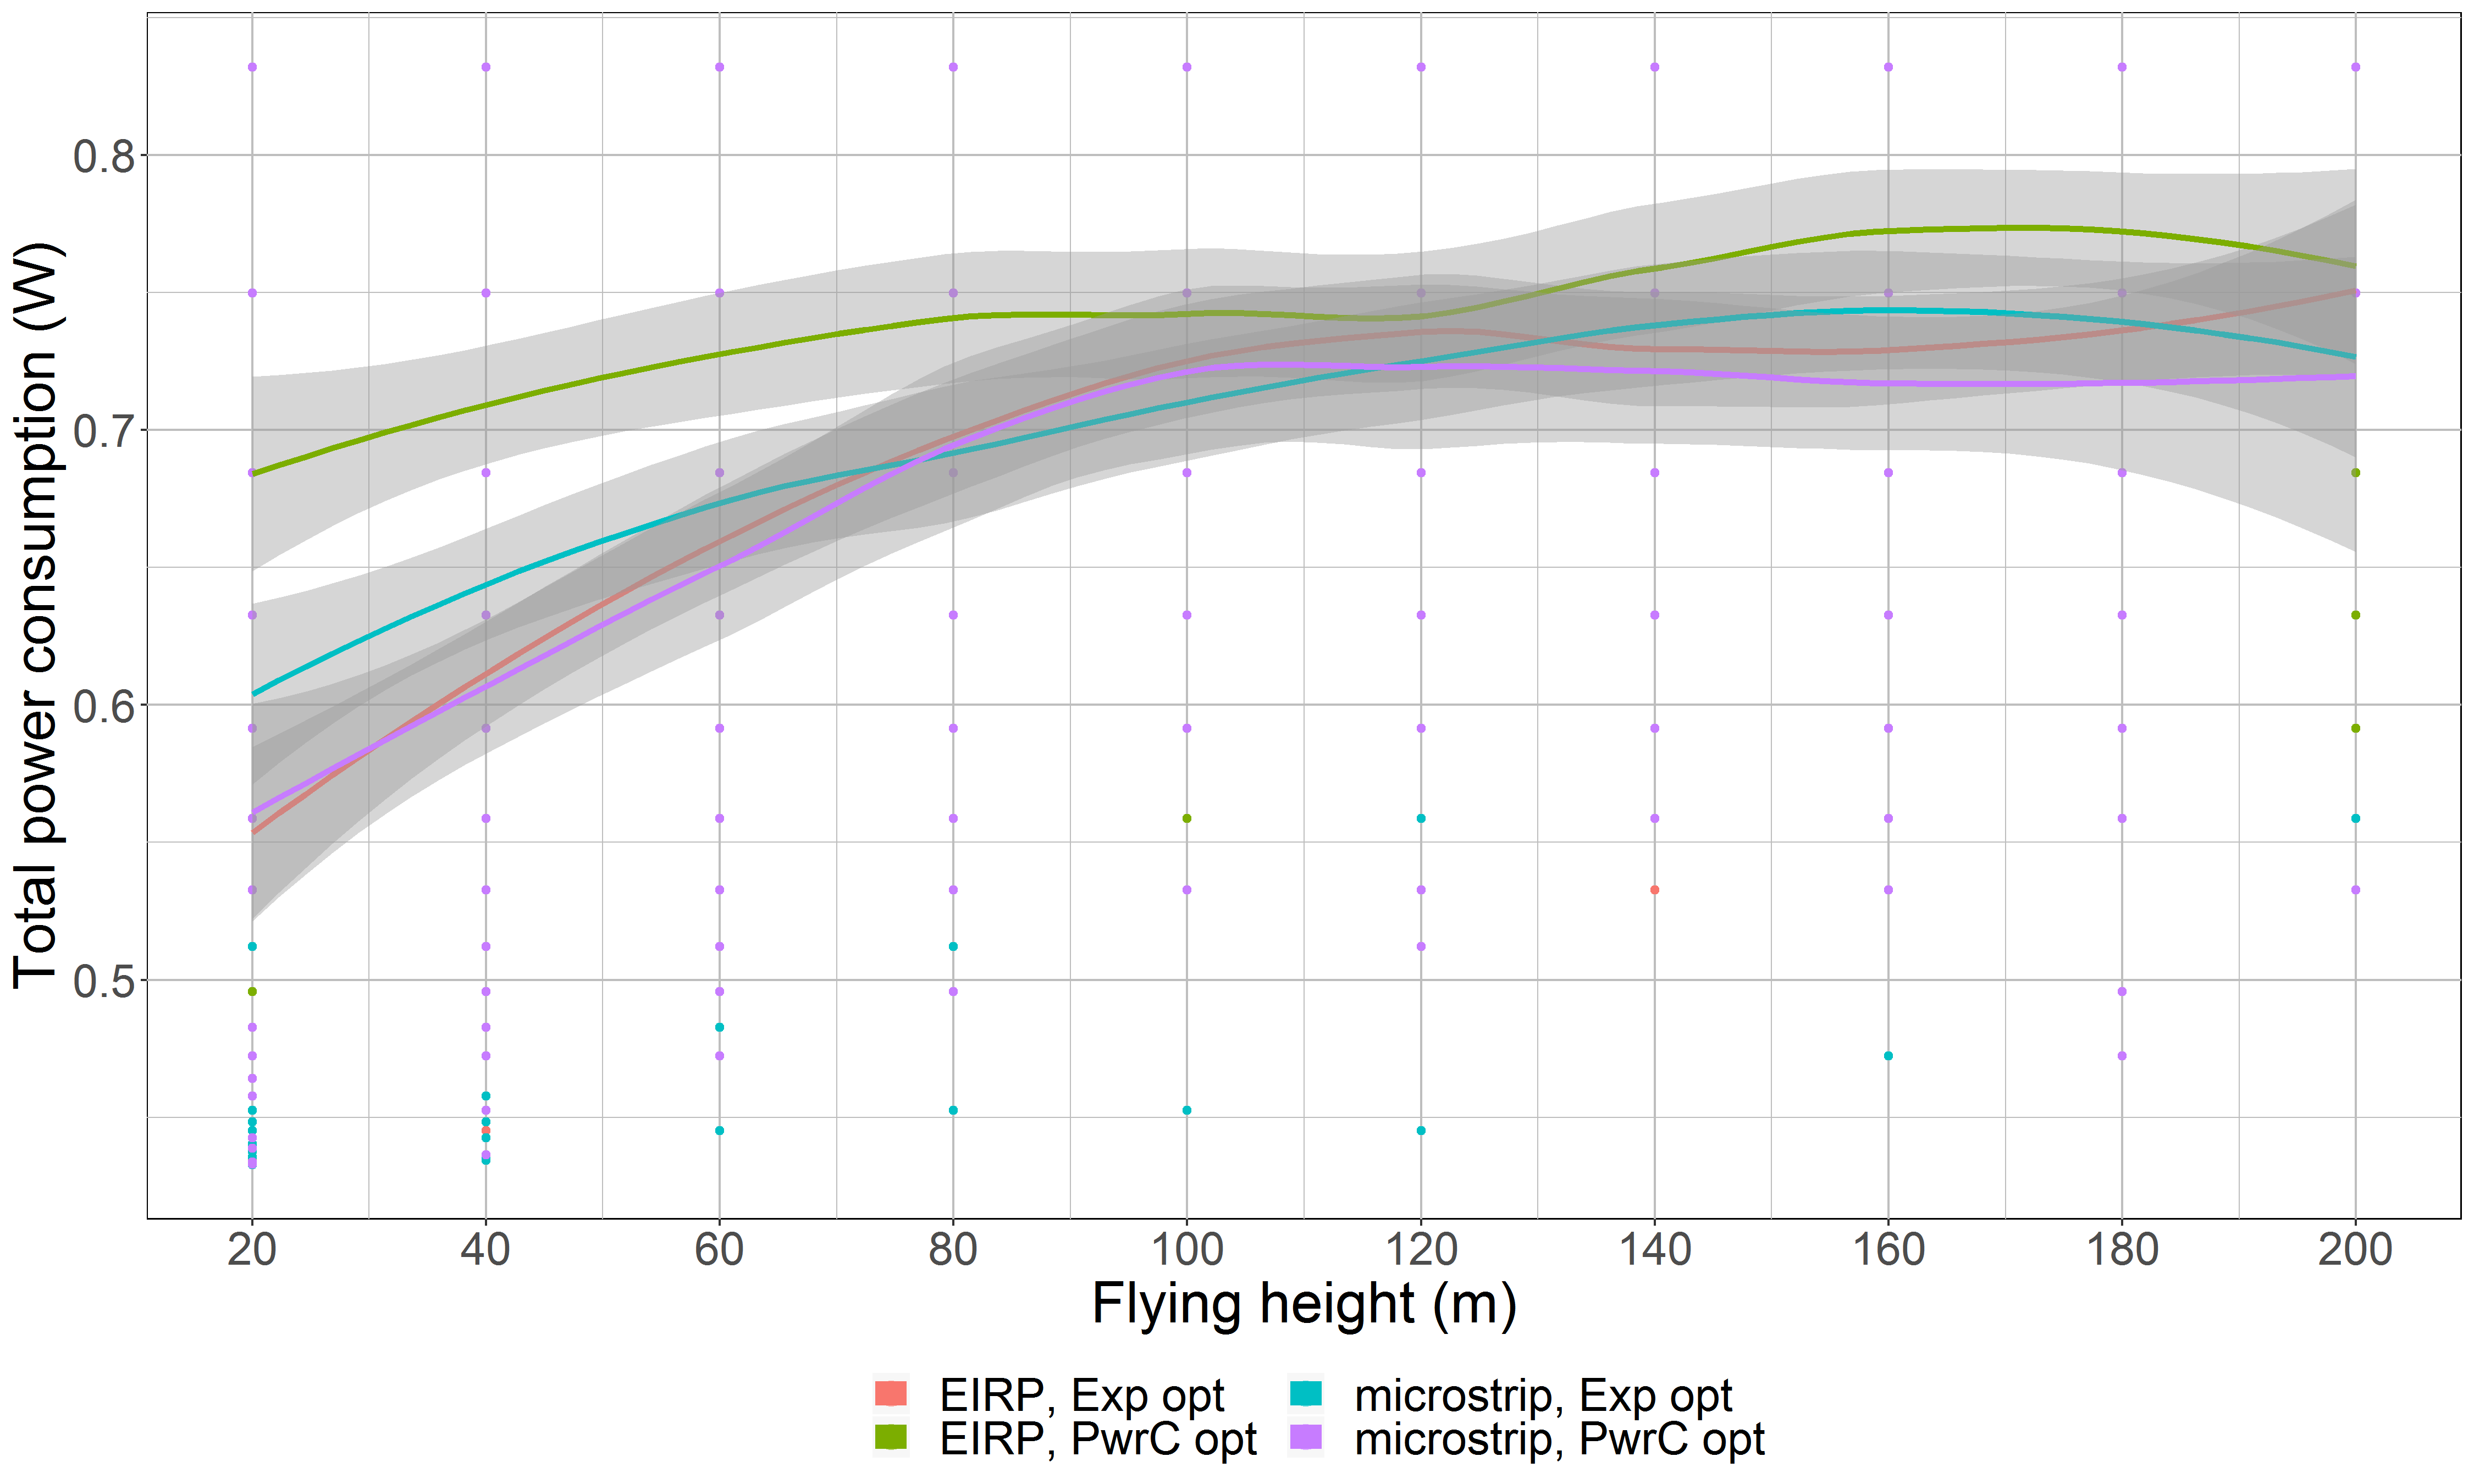
\includegraphics[width=\textwidth]{../results/s2/fhvsdlAndPc.png}
  \caption{The influence of the flying height on the weighted average downlink exposure of users in the network.}
  \label{fig:s2a_dlAndPc}
\end{figure}



%\newpage
The \gls{DL} exposure in figure \ref{fig:s2a_dlAndPc} increases along with the flying height. One might expect a more constant 
behaviour like it was the case in figure \ref{fig:s1_fhsar} of scenario 1. To understand this, the scenario has been deducted 
with only two users and is illustrated in figure \ref{fig:schematicprove}.
The two users, who will be referred to by `red' and `blue', are 90 metres separated from each other with a building between them.
Scenario 1 already explained that the charts can be simplified and the blue line from fig. \ref{fig:prove} remains in fact constant between the zero and 130 metres.
The chart shows that the \gls{UABS} is positioned above the blue user. The red user is in \gls{NLOS} as long as the \gls{UABS} remains below 20 metres.

\begin{figure}[]
  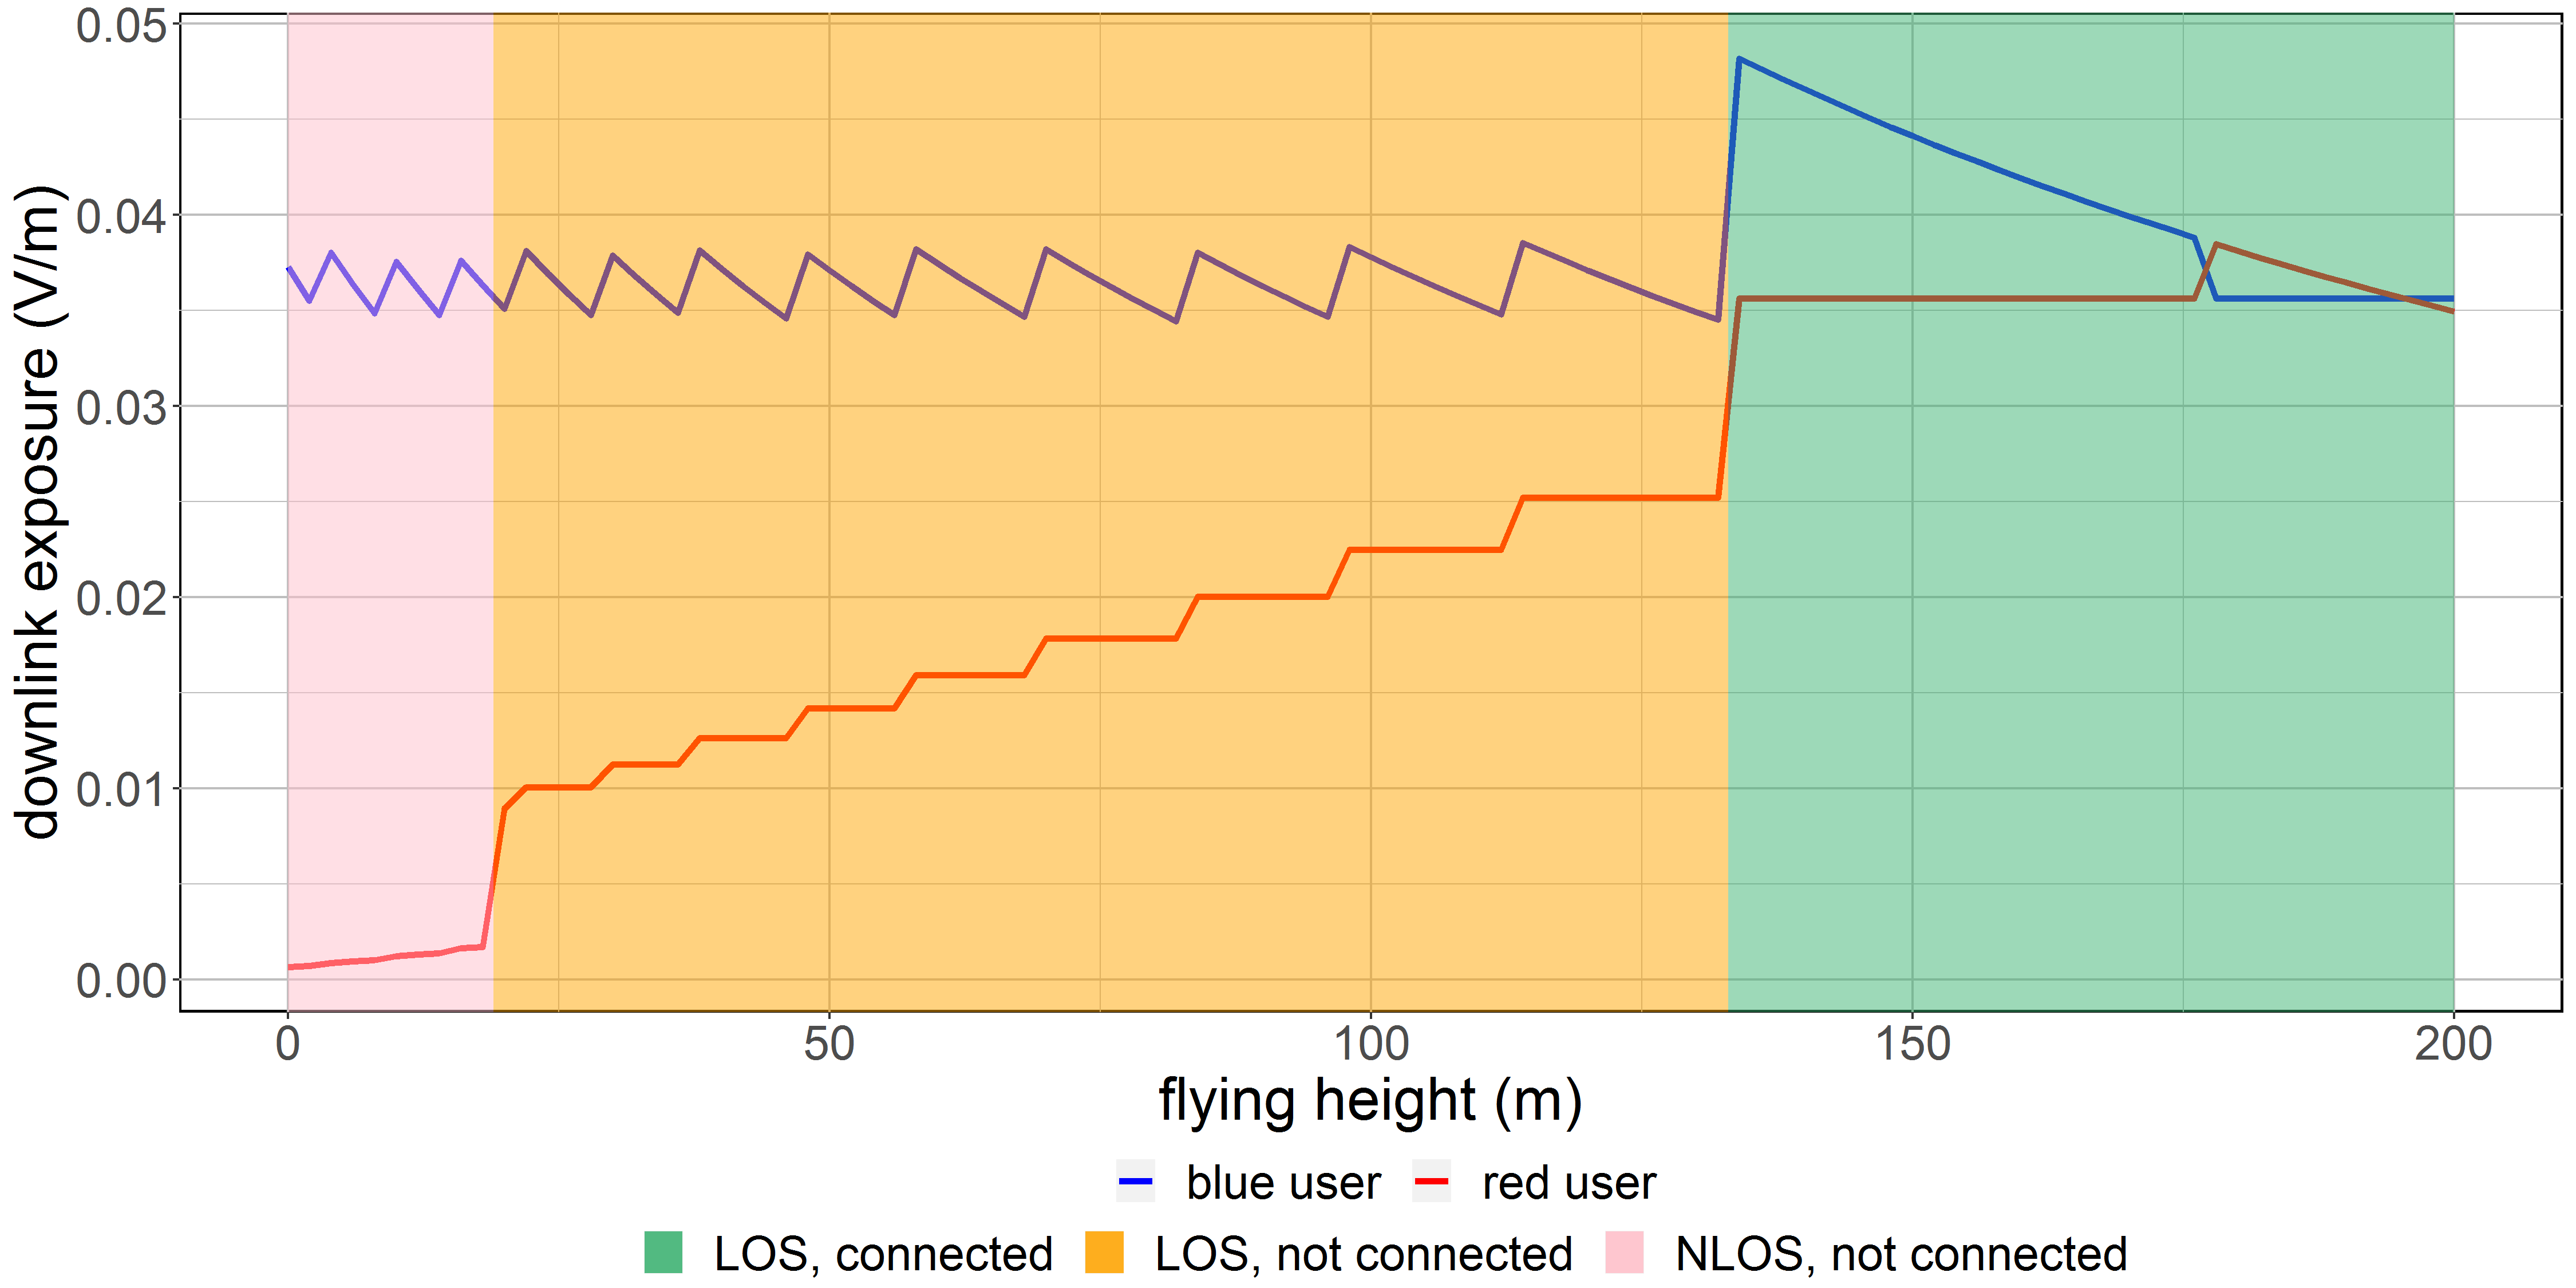
\includegraphics[width=\textwidth]{../results/s2/prove.png}
  \caption{Scenario 2 with only 2 users. The coloured areas are only applicable for the red user. The blue user is connected during the entire time.}
  \label{fig:prove}
\end{figure}


\begin{wrapfigure}{r}{0.48\textwidth}
  \begin{center}
    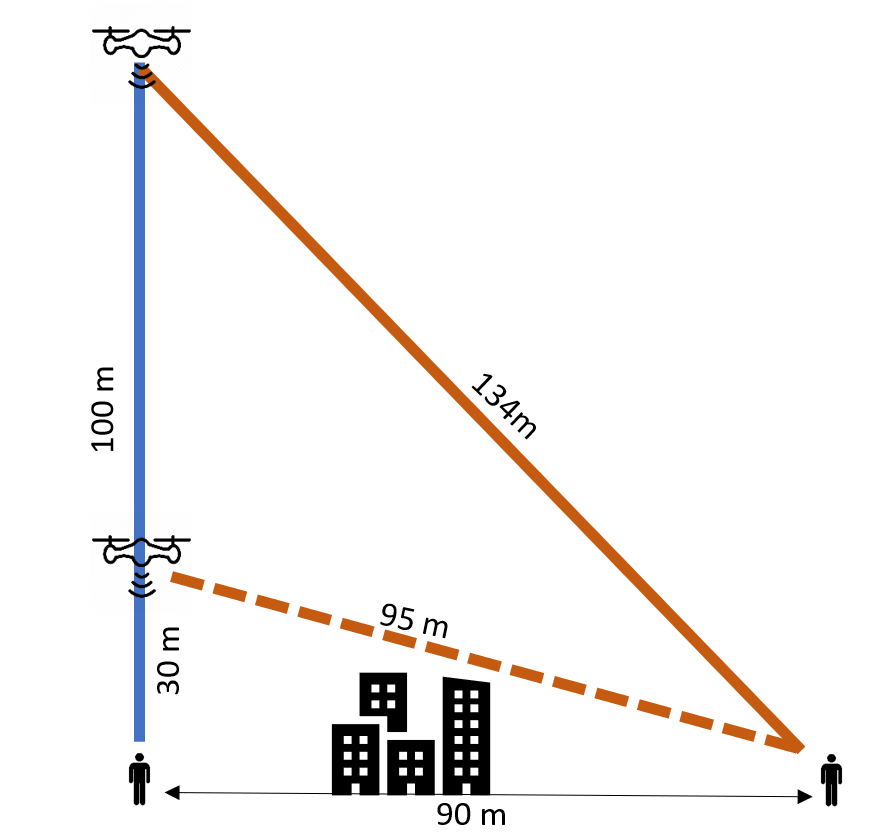
\includegraphics[width=0.48\textwidth]{../results/s2/proveScenario.png}
  \end{center}
  \caption{Schematic overview of scenario 2 with only 2 users.}
  \label{fig:schematicprove}
\end{wrapfigure}
Once the \gls{UABS} increases its flying altitude, the red user becomes into \gls{LOS} but still remains uncovered. This is because the tool initially locate a possible 
\gls{UABS} above each user and thereafter performs the  fitness function. The applied fitness function must have decided that it is better to connect 
each user to the \gls{UABS} above him. At a final state, the tool check whether the number of online \gls{UAV}s does not exceed the capacity of the facility
which is here the case. The tool therefore deactivates one \gls{UABS} causing the red user to be uncovered. One could argue that the 
the red user should be connected to the online \gls{UAV} who is only 90 metres away. This would however require the online \gls{UAV} to increase his power consumption which 
would make the decisions made by the optimization strategy obsolete.
When the \gls{UAV} flies higher, the difference in distance between both users and the base station decreases. In other words, the Pythagorean theorem shows that when the flying height of the 
\gls{UABS} increases, the distance with the blue user increases faster compared to the distance between that same \gls{UABS} and the red user. This is also illustrated in figure \ref{fig:schematicprove}.
At 130 metres, the tool decides to connect both users to the same \gls{UABS}. Therefore, it increases it's power consumption so the red user would  have the minimal 
required electromagnetic exposure. This has of course a negative influence for the blue user who is way closer and experience now a much higher exposure level in fig \ref{fig:prove}.
Around 180 metres, the  red and blue line switch because the \gls{UAV} changes position. As explained before, the tool assigns two possible \gls{UAV}s, one above 
each user. The tool must have decided that connecting both users to the other \gls{UAV}s improves the fitness function of the entire network even though that difference might be 
very little. \\
Finally, brings us back to figure \ref{fig:s2a_dlAndPc} where the electromagnetic exposure in the weighed average of all users. In other words, there are 223 users who behave like the  red user while only
one user behaves like the blue one. 
The red line therefore dominates the average exposure in figures \ref{fig:s2a_dlAndPc}.

\begin{figure}[h]
  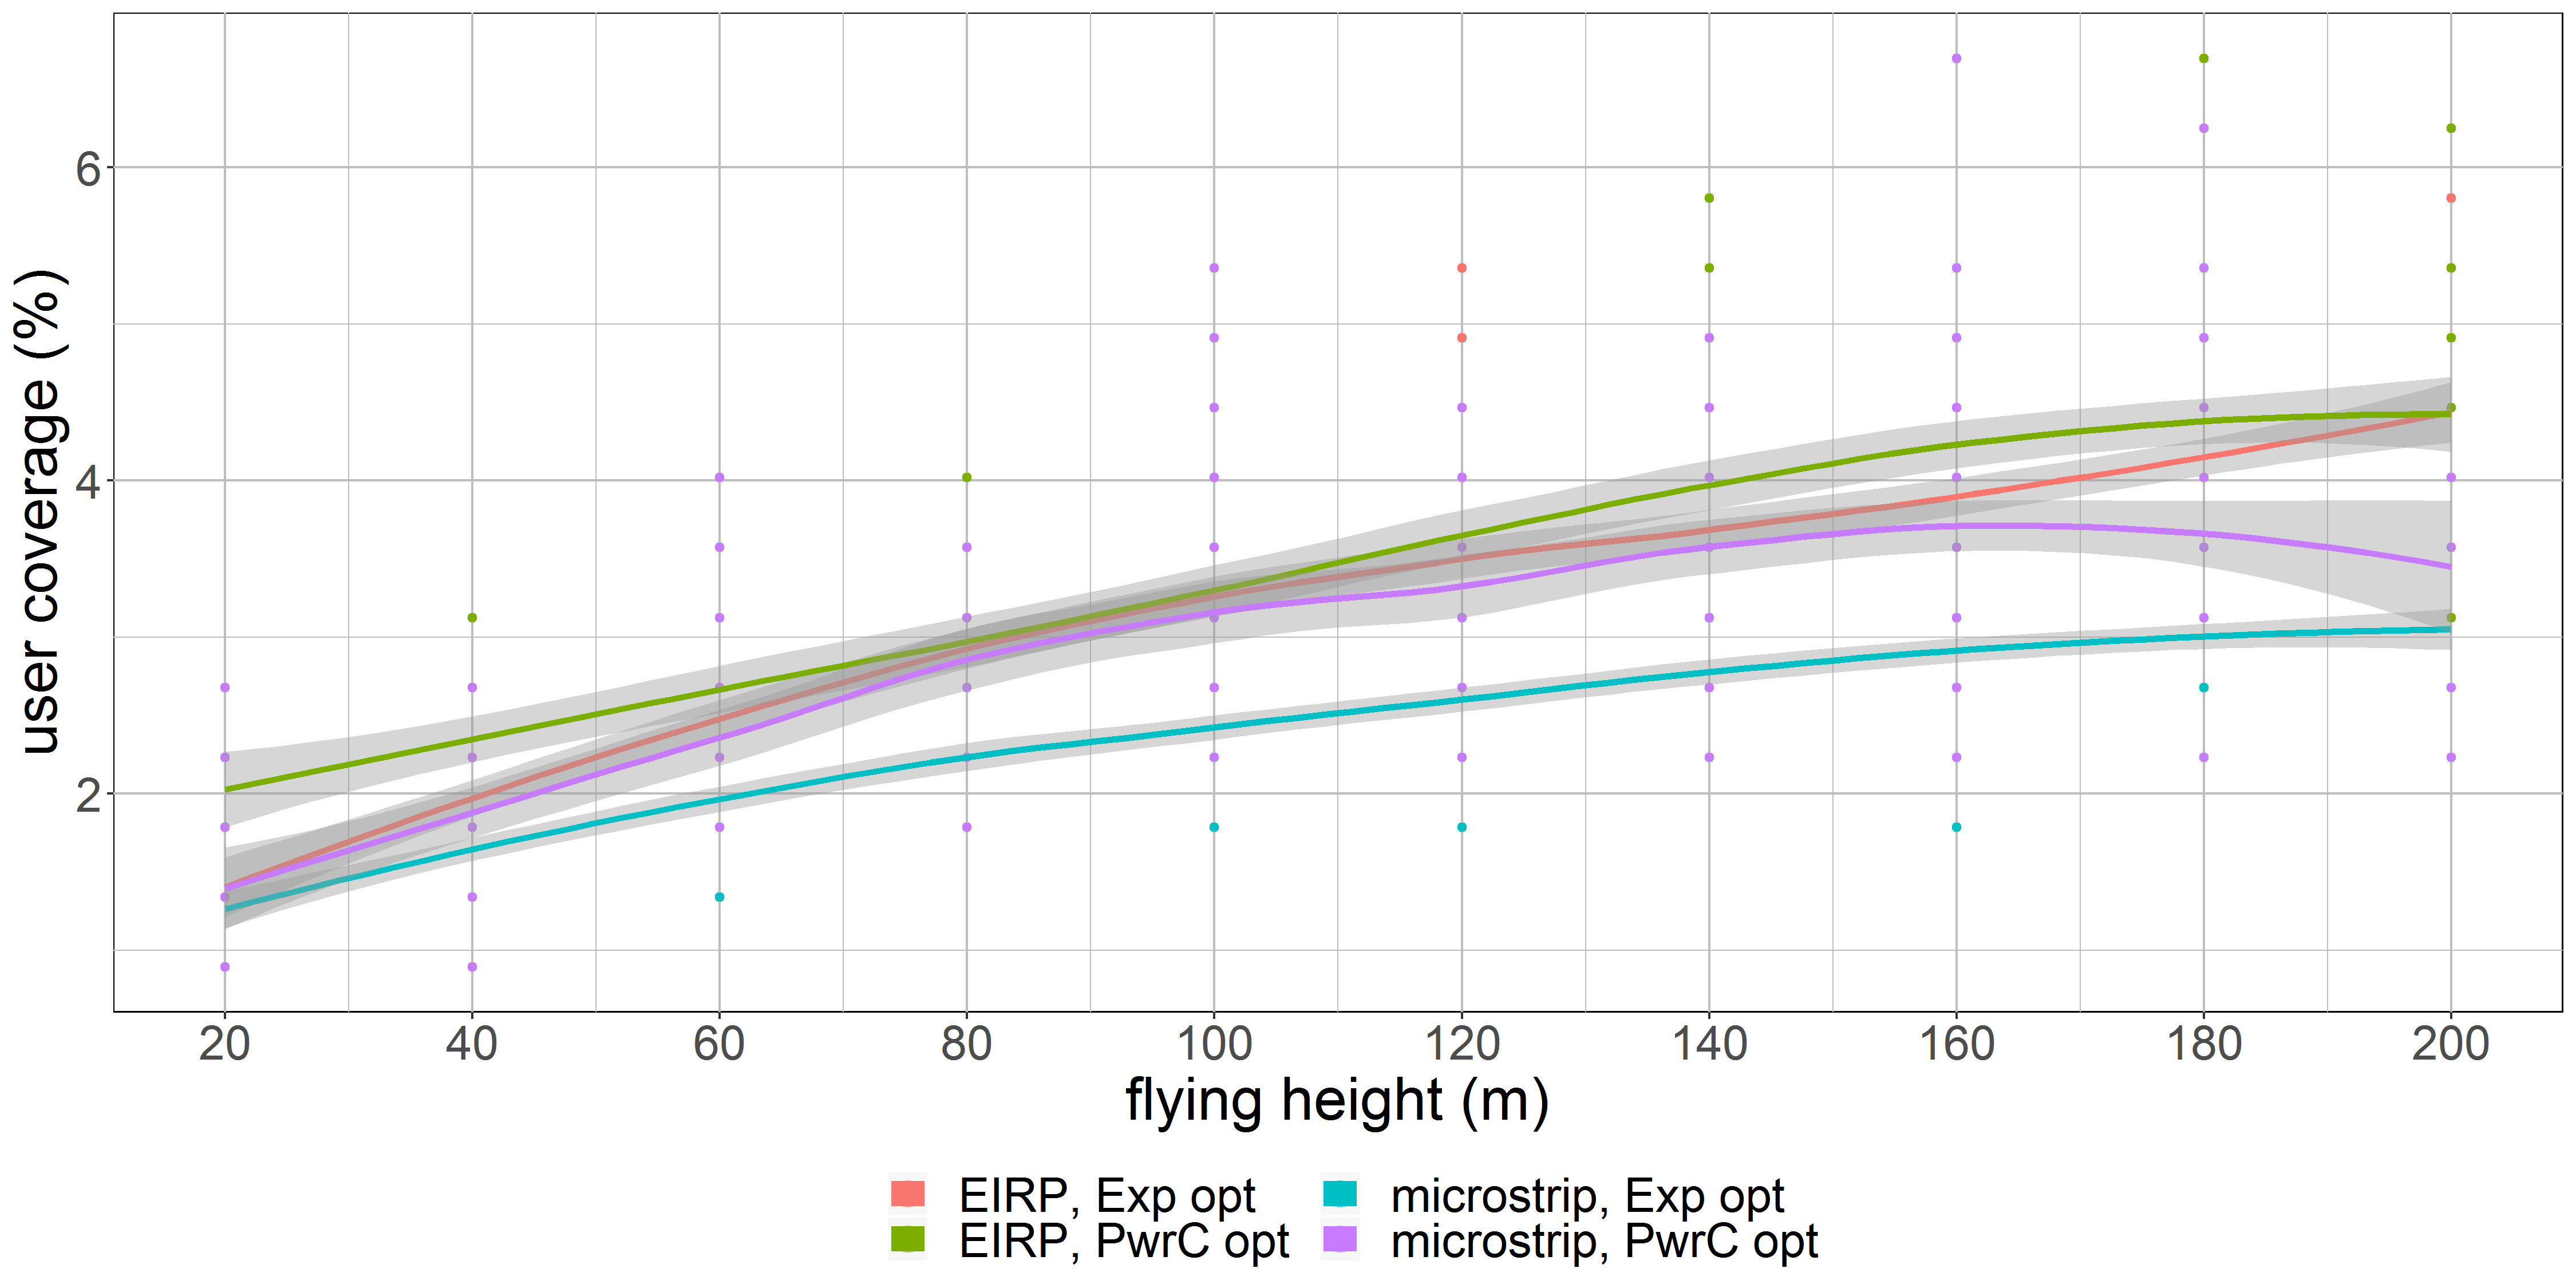
\includegraphics[width=\textwidth]{../results/s2/fhvscov.png}
  \caption{This graph shows the percentage of covered users by one \gls{UAV} for different flying heights.}
  \label{fig:s2fhvscov}
\end{figure}

Figure  \ref{fig:s2fhvscov} shows that the flying height has a positive influence on the user coverage. 
When a \gls{UABS} flies higher, there is less path loss between the user and the \gls{UAV} caused by buildings but also the path loss to neighbouring 
users decreases as explained 
with figure \ref{fig:prove} and \ref{fig:schematicprove}. 
Also the increasing \gls{DL} exposure  from figure \ref{fig:s2a_dlAndPc} from earlier indicated that the
user coverage should grow.

When replacing the fictional \gls{EIRP} antenna with a microstrip patch antenna, the percentage of covered users drops for both 
optimization strategies. This is because users who have a higher horizontal distance between themselves and the \gls{UABS}, 
experience a higher attenuation. When a microstrip patch antenna is positioned higher, the range of the antenna increases 
since the angle between the user and the \gls{UABS}s main lob decreases. The user will therefore experience less attenuation.

Eventually, figure \ref{fig:s2shfourSourcesMatrix} shows the total whole body $SAR_{10g}$, deducted from all electromagnetic sources. This being the exposure 
of the only \gls{UABS} available in the network, 
 the \gls{UL} exposure from the user’s own device and the exposure of the devices from all other users. 
 Thereafter, the weighted average whole body \gls{SAR} for each individual source in the network is calculated with the 50th and 95th percentile 
 being the most important values. This is because not only the mean value is important but also users who experience higher 
 levels of whole body $SAR_{10g}$.

When investigating the three different sources of which the total \gls{SAR}-values are based on, we see 
that the radiation from the \gls{UABS} is the main factor followed by the near field radiation from the user's own device.
The far field radiation from other \gls{UE} has barely influence. 
It looks like it is zero but it is just very low compared to the other two values and in fact does increases when the flying height becomes larger.

The weighted average $SAR^{ul}_{10g}$ from the own device is zero in an exposure optimized network with a microstrip patch antenna which is even lower that the $SAR^{neighbours}_{10g}$.
This is because the coverage in this scenario is so low that the weighted average only consist of uncovered users and an uncovered user his device has no power consumption.
\begin{figure}[]
  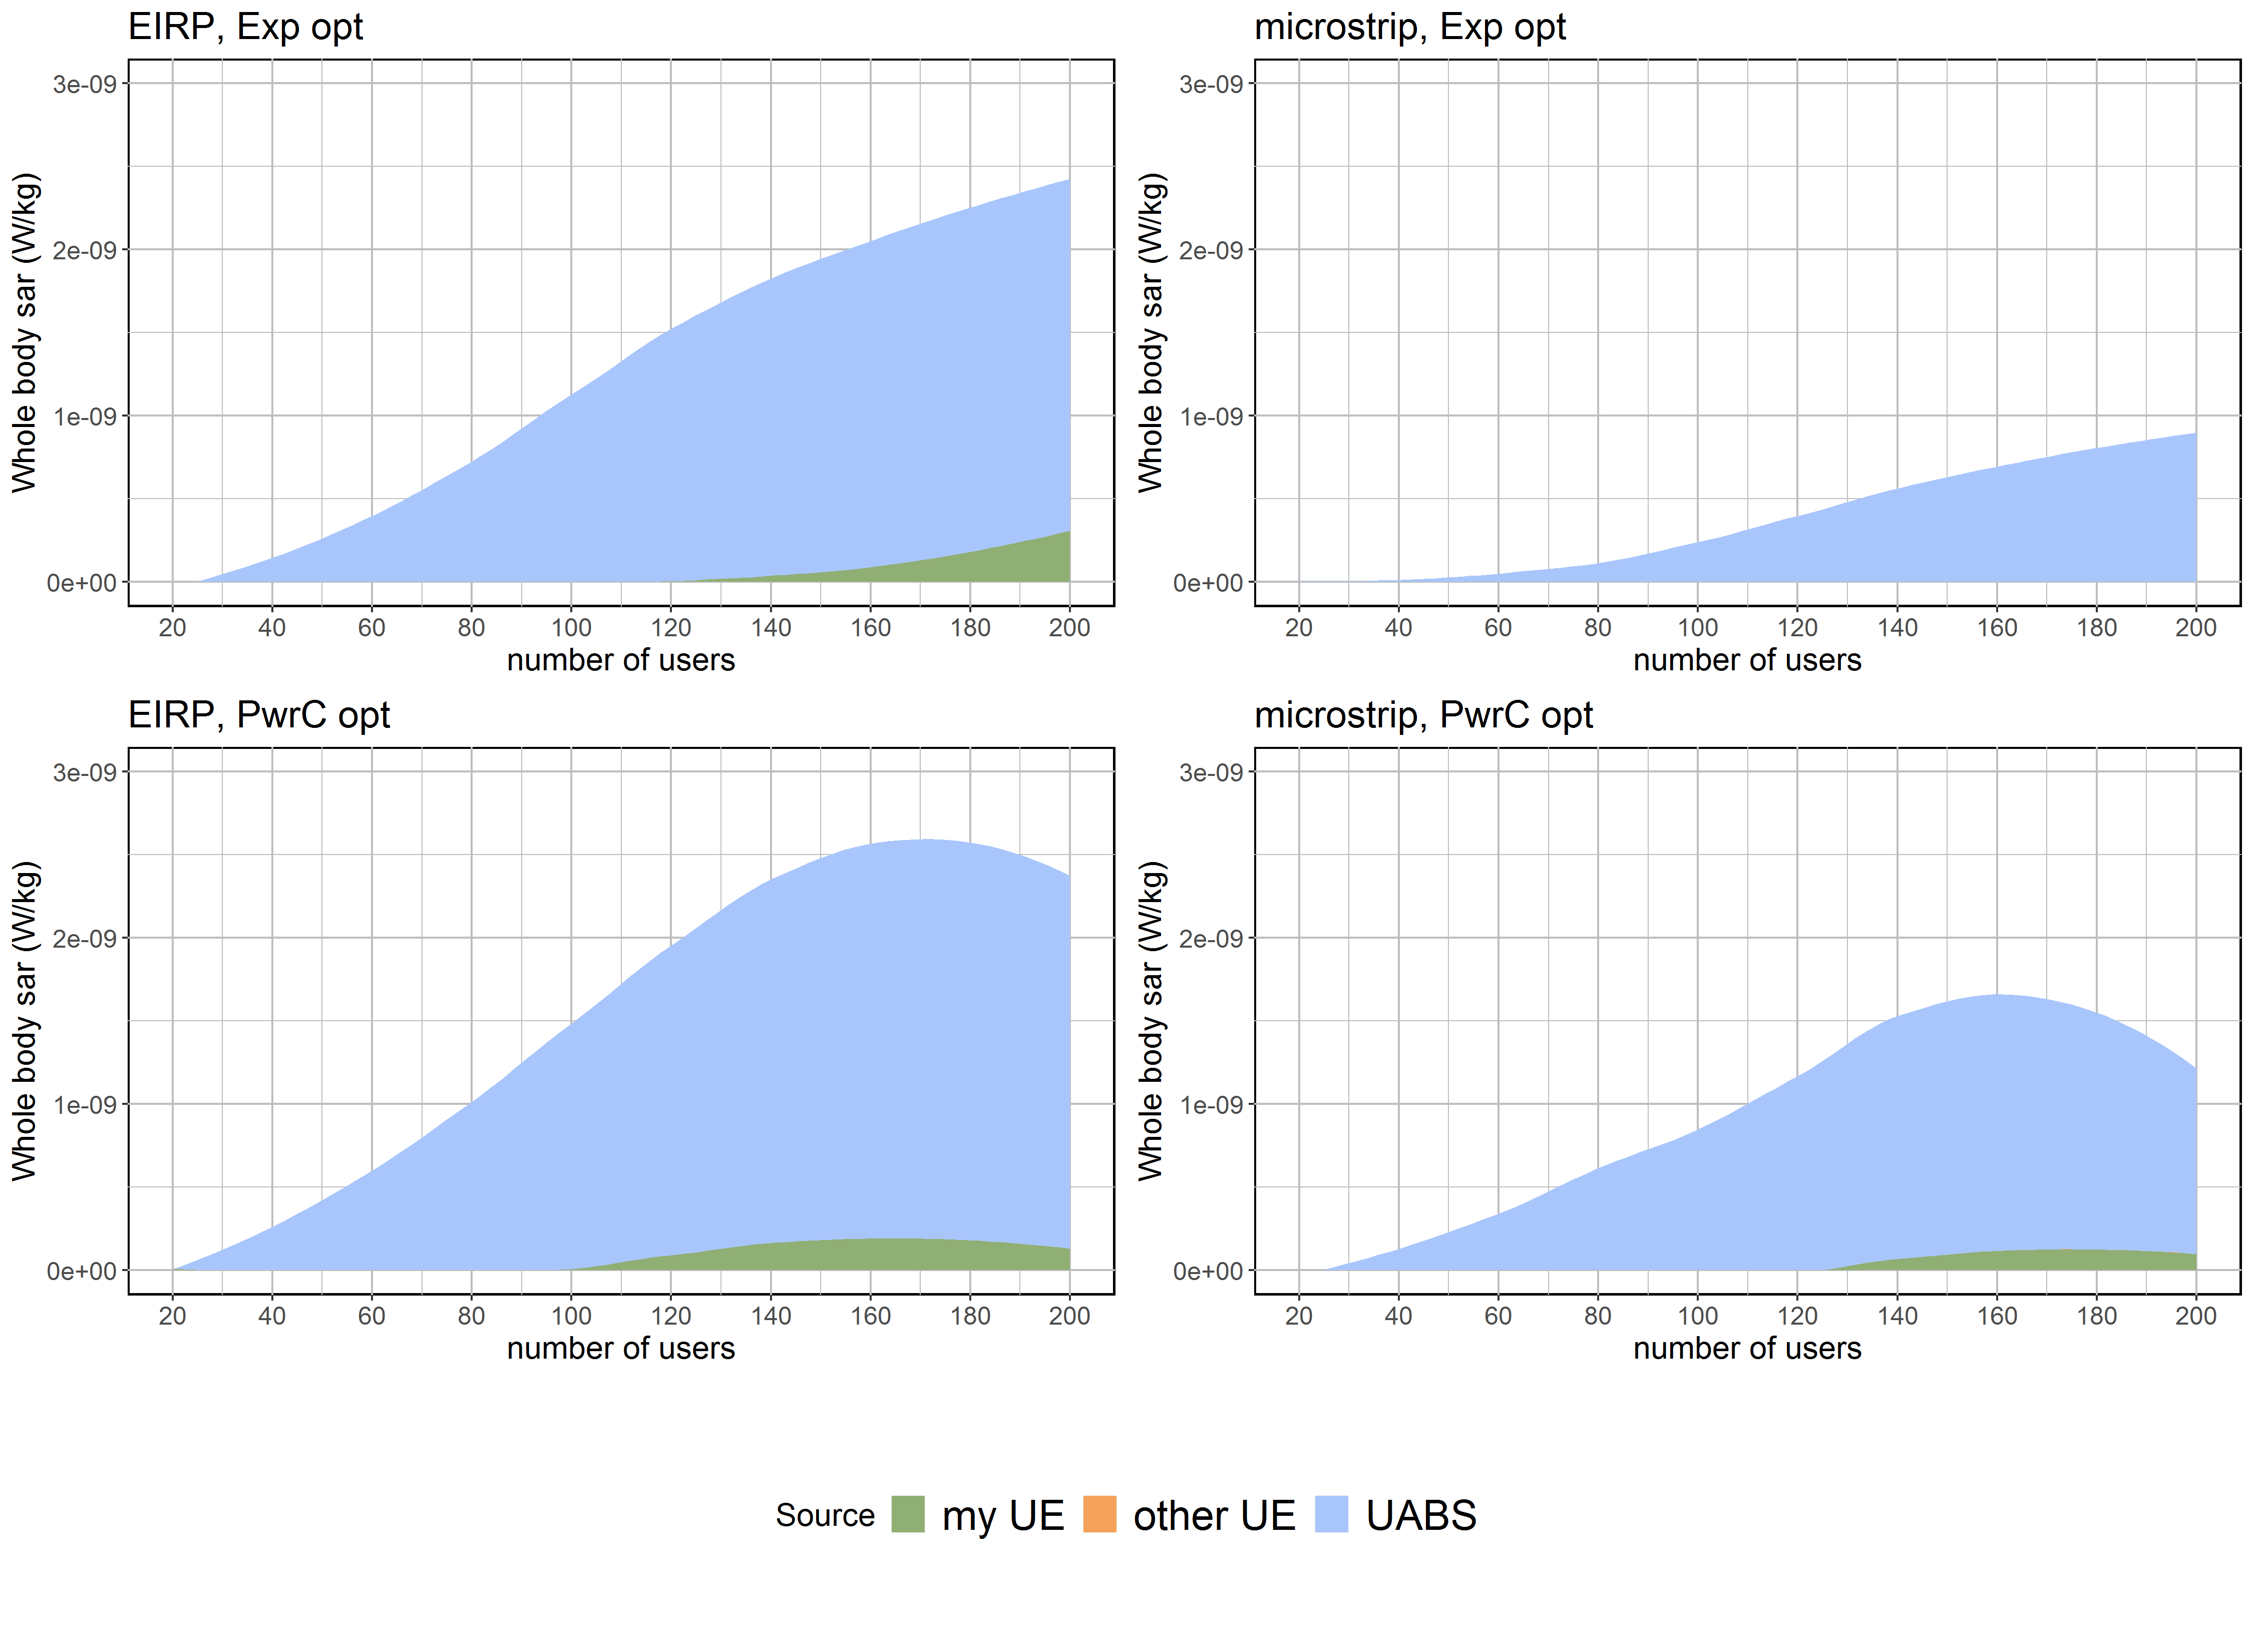
\includegraphics[width=\textwidth]{../results/s2/fhFourSources.png}
  \caption{This figure shows how different sources are influenced by an increasing flying height.}
  \label{fig:s2shfourSourcesMatrix}
\end{figure}

%%%%%%%%%%%%%%%%%%%%%%%%%%%%%%%%%%%%%%%%%%%%%%%%%%%%%%%%%%%%%%%%%%%%%%%%%%%%%%%%%%%%%%%%%%%%%%%%%%%%%%%%
\FloatBarrier
\subsection{Influence of the Number of Users}
\label{s2b}

The number of covered users increase linearly compared to the number of users present in the network as shown in figure 
\ref{fig:s2uvsnumcovusers} on the right. It illustrates how an \gls{isotropicradiator} is able of reaching more users 
compared to a microstrip patch antennae.
Also, power consumption optimized networks are able of reaching more users compared to exposure optimized networks.
This is because power consumption optimized network will result in few high powered base station while an 
exposure optimized network result in a lot of low powered base stations. This behaviour will further be explained in section \ref{s3}

\begin{figure}[h!]
  \includegraphics[width=\textwidth]{../results/s2/uvsnum\gls{UAV}sAndCov.png}
  \caption{The influence of increasing traffic on user coverage.}
  \label{fig:s2uvsnumcovusers}
\end{figure}

The linear regression lines from \ref{fig:s2uvsnumcovusers} can be predicted with the equations in \ref{eq:numcovusers}.

\begin{equation}
\text{number of users =}
    \begin{cases}
      y = 0,0233x + 2,3553 & \text{if EIRP and pc}\\
      y = 0,0197x + 2,6144  & \text{if EIRP and exp}\\
      y = 0,0131x + 2,4371  & \text{if micro and pc}\\
      y = 0,0119x + 2,4652  & \text{if micro and exp}
    \end{cases} 
    \label{eq:numcovusers}      
\end{equation}

Figure \ref{fig:s2uvsnumcovusers} on the left show the percentage of covered users that follows out of \ref{fig:s2uvsnumcovusers} on the right by taking the equations from \ref{eq:numcovusers} and dividing them by $x$.
This results in a decreasing logarithmic behaviour because the regression lines from  \ref{fig:s2uvsnumcovusers} have a slope of less then 0.5.
So in other words, the  percentage of covered users for a sparsely populated network is more compared to the percentage of users in high dense populations.

\begin{figure}[h!]
  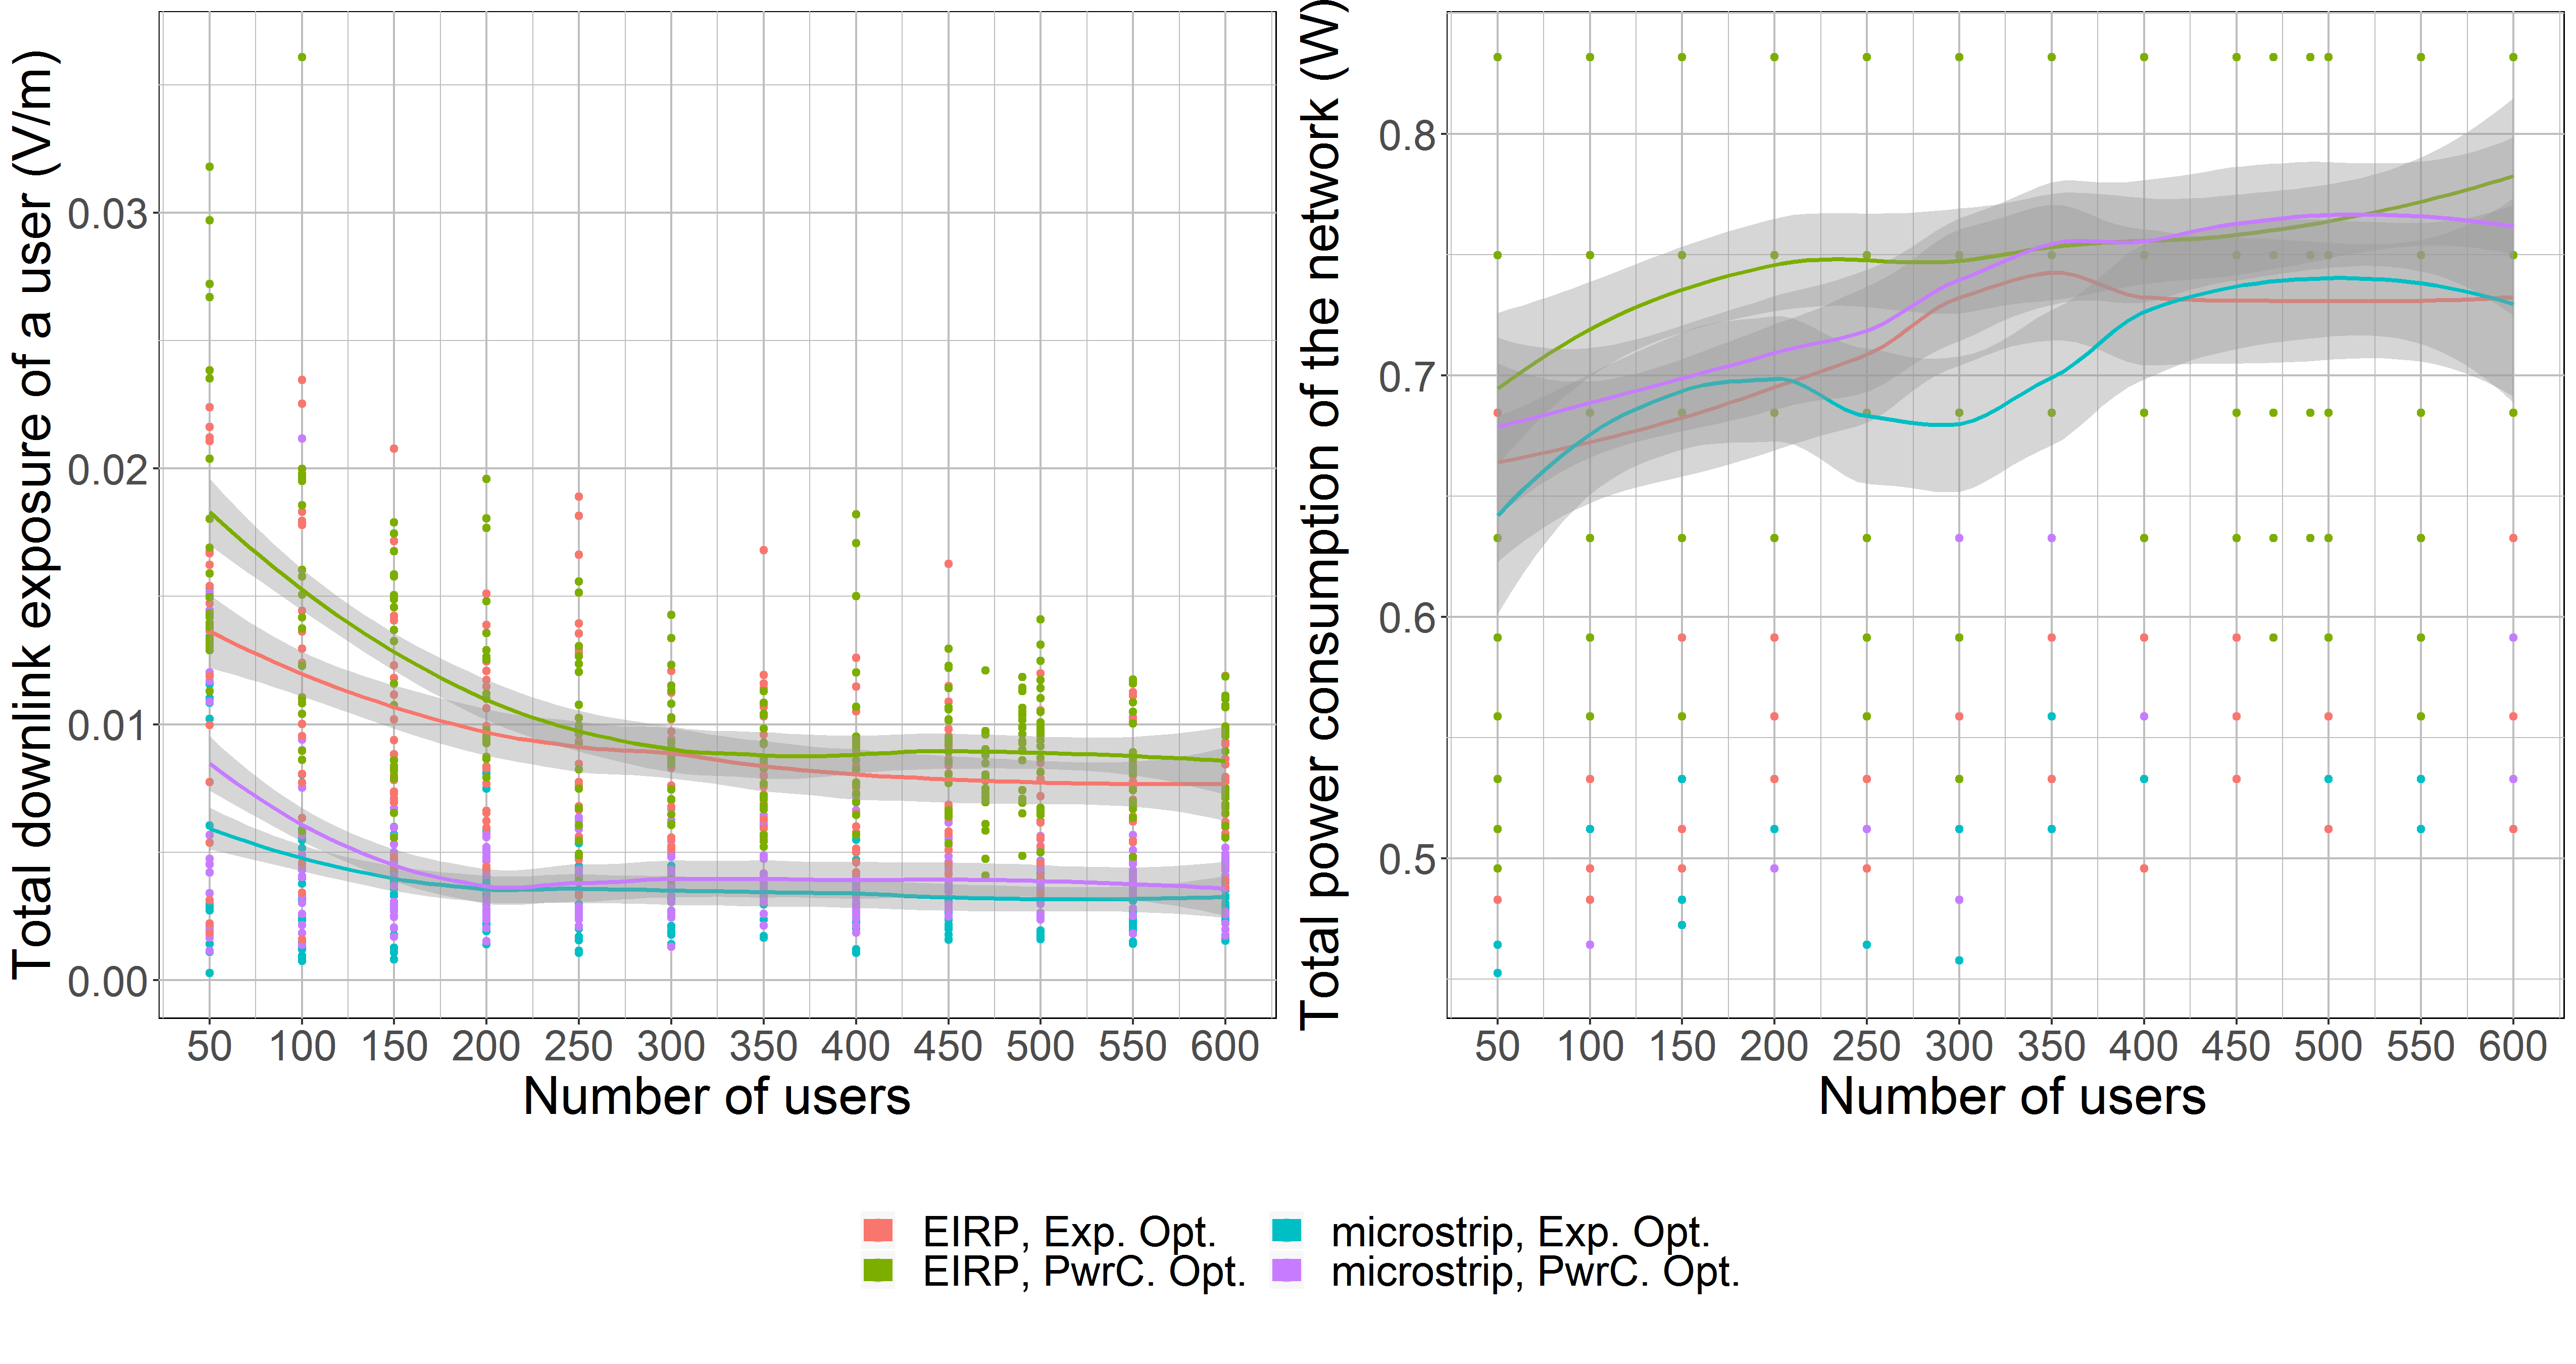
\includegraphics[width=\textwidth]{../results/s2/uvsdlAndPc.png}
  \caption{This figure shows how different sources are influenced by an increasing number of users. }
  \label{fig:s2b_dlAndPc}
\end{figure}

The downlink exposure is shown in figure \ref{fig:s2b_dlAndPc} on the left and is directly influenced by the percentage of covered users. 
The average electromagnetic exposure decreases when more users become uncovered. Since an \gls{isotropicradiator} in a power consumption optimized network (green)
will have the highest coverage, also the \gls{DL} electromagnetic radiation from \gls{UABS}s will be higher compared to other configurations.
Despite the fact that the percentage of covered users decreases, the effective number of covered users increases. The power consumption of the only 
active \gls{UABS} slightly increases in order to serve those covered users.


Figure \ref{fig:s2fourSourcesMatrix} investigates the assets of each source contributing to the total \gls{SAR}. All four 
configurations show that base stations are the main source of electromagnetic radiation.
Figure \ref{fig:s2uvsnumcovusers} already 
showed that for sparsely populated networks, a higher percentage is covered so the weighted average of the \gls{UL} \gls{SAR} will also be higher. 
When the population becomes more dense,
more users become uncovered which decreases the weighted average of the \gls{UL} \gls{SAR}.
The chart also proves once again that the far field radiation from \gls{UE} can be neglected. The \gls{SAR} from 
neighbouring devices is not zero as it looks from figure \ref{fig:s2fourSourcesMatrix} but is just really low compared to the much higher
\gls{SAR}-values from other sources.

\begin{figure}[h!]
\centering
  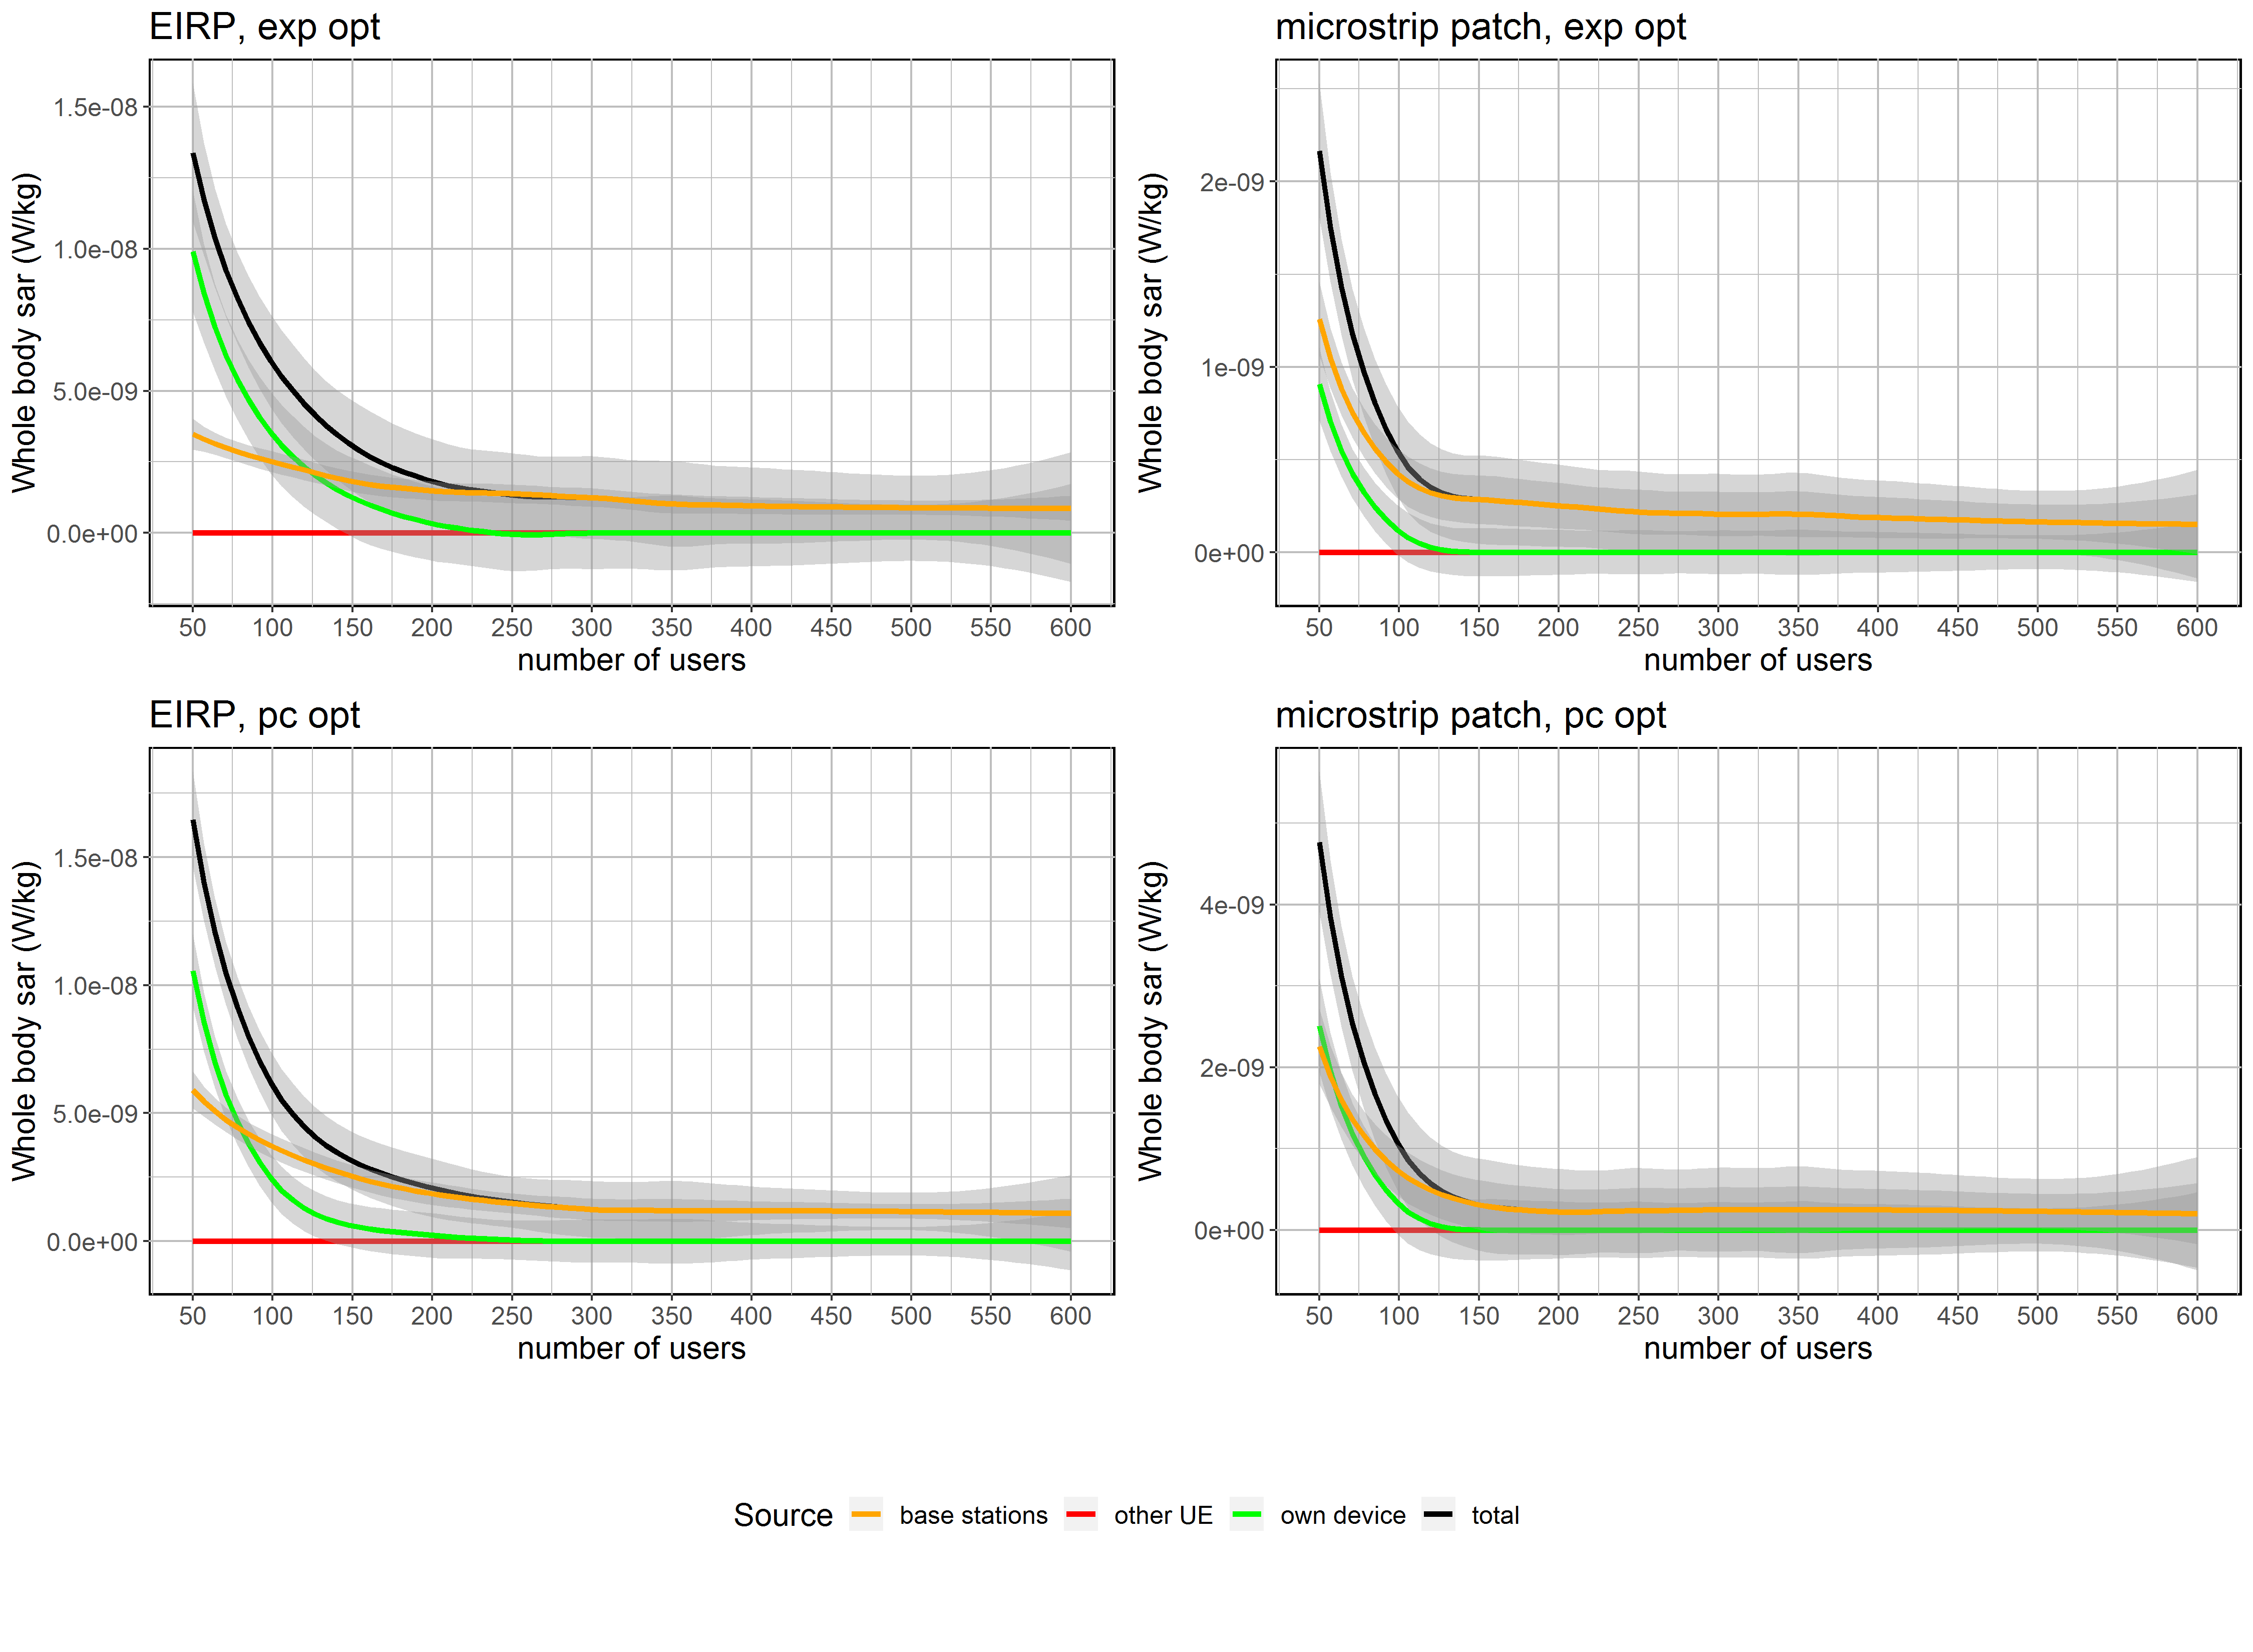
\includegraphics[width=\textwidth/6*5]{../results/s2/uFourSources.png}
  \caption{This figure shows how different sources are influenced by an increasing number of users. }
  \label{fig:s2fourSourcesMatrix}
\end{figure}

While the population grows, more and more users become uncovered causing the average SAR to drop. However, this does not conclude that the same applies for 
users who are covered. To investigate this, a user is positioned in the middle of the city center of Ghent and a \gls{UAV} is positioned above him. Initially, only 
49 people are active around him. The \gls{SAR} of our central user is monitored while the population around him grows.
Figure \ref{fig:connectionMap} shows with the black lines which users are connected. The left map is for only 50 users and 
shows that only one user is connected besides our central user. The map on the right is taken with 600 users and shows much more connected users.



It might look that by increasing the population, the SAR of a user who is directly beneath a \gls{UABS} would be less but that is 
certainly not the case as demonstrated in the experiment below. A central user will be placed in the middle of Ghent with one \gls{UAV} above him.
The different \gls{SAR}-values of this central user are monitored while the population around him grows.

\begin{figure}[h!]
\centering
  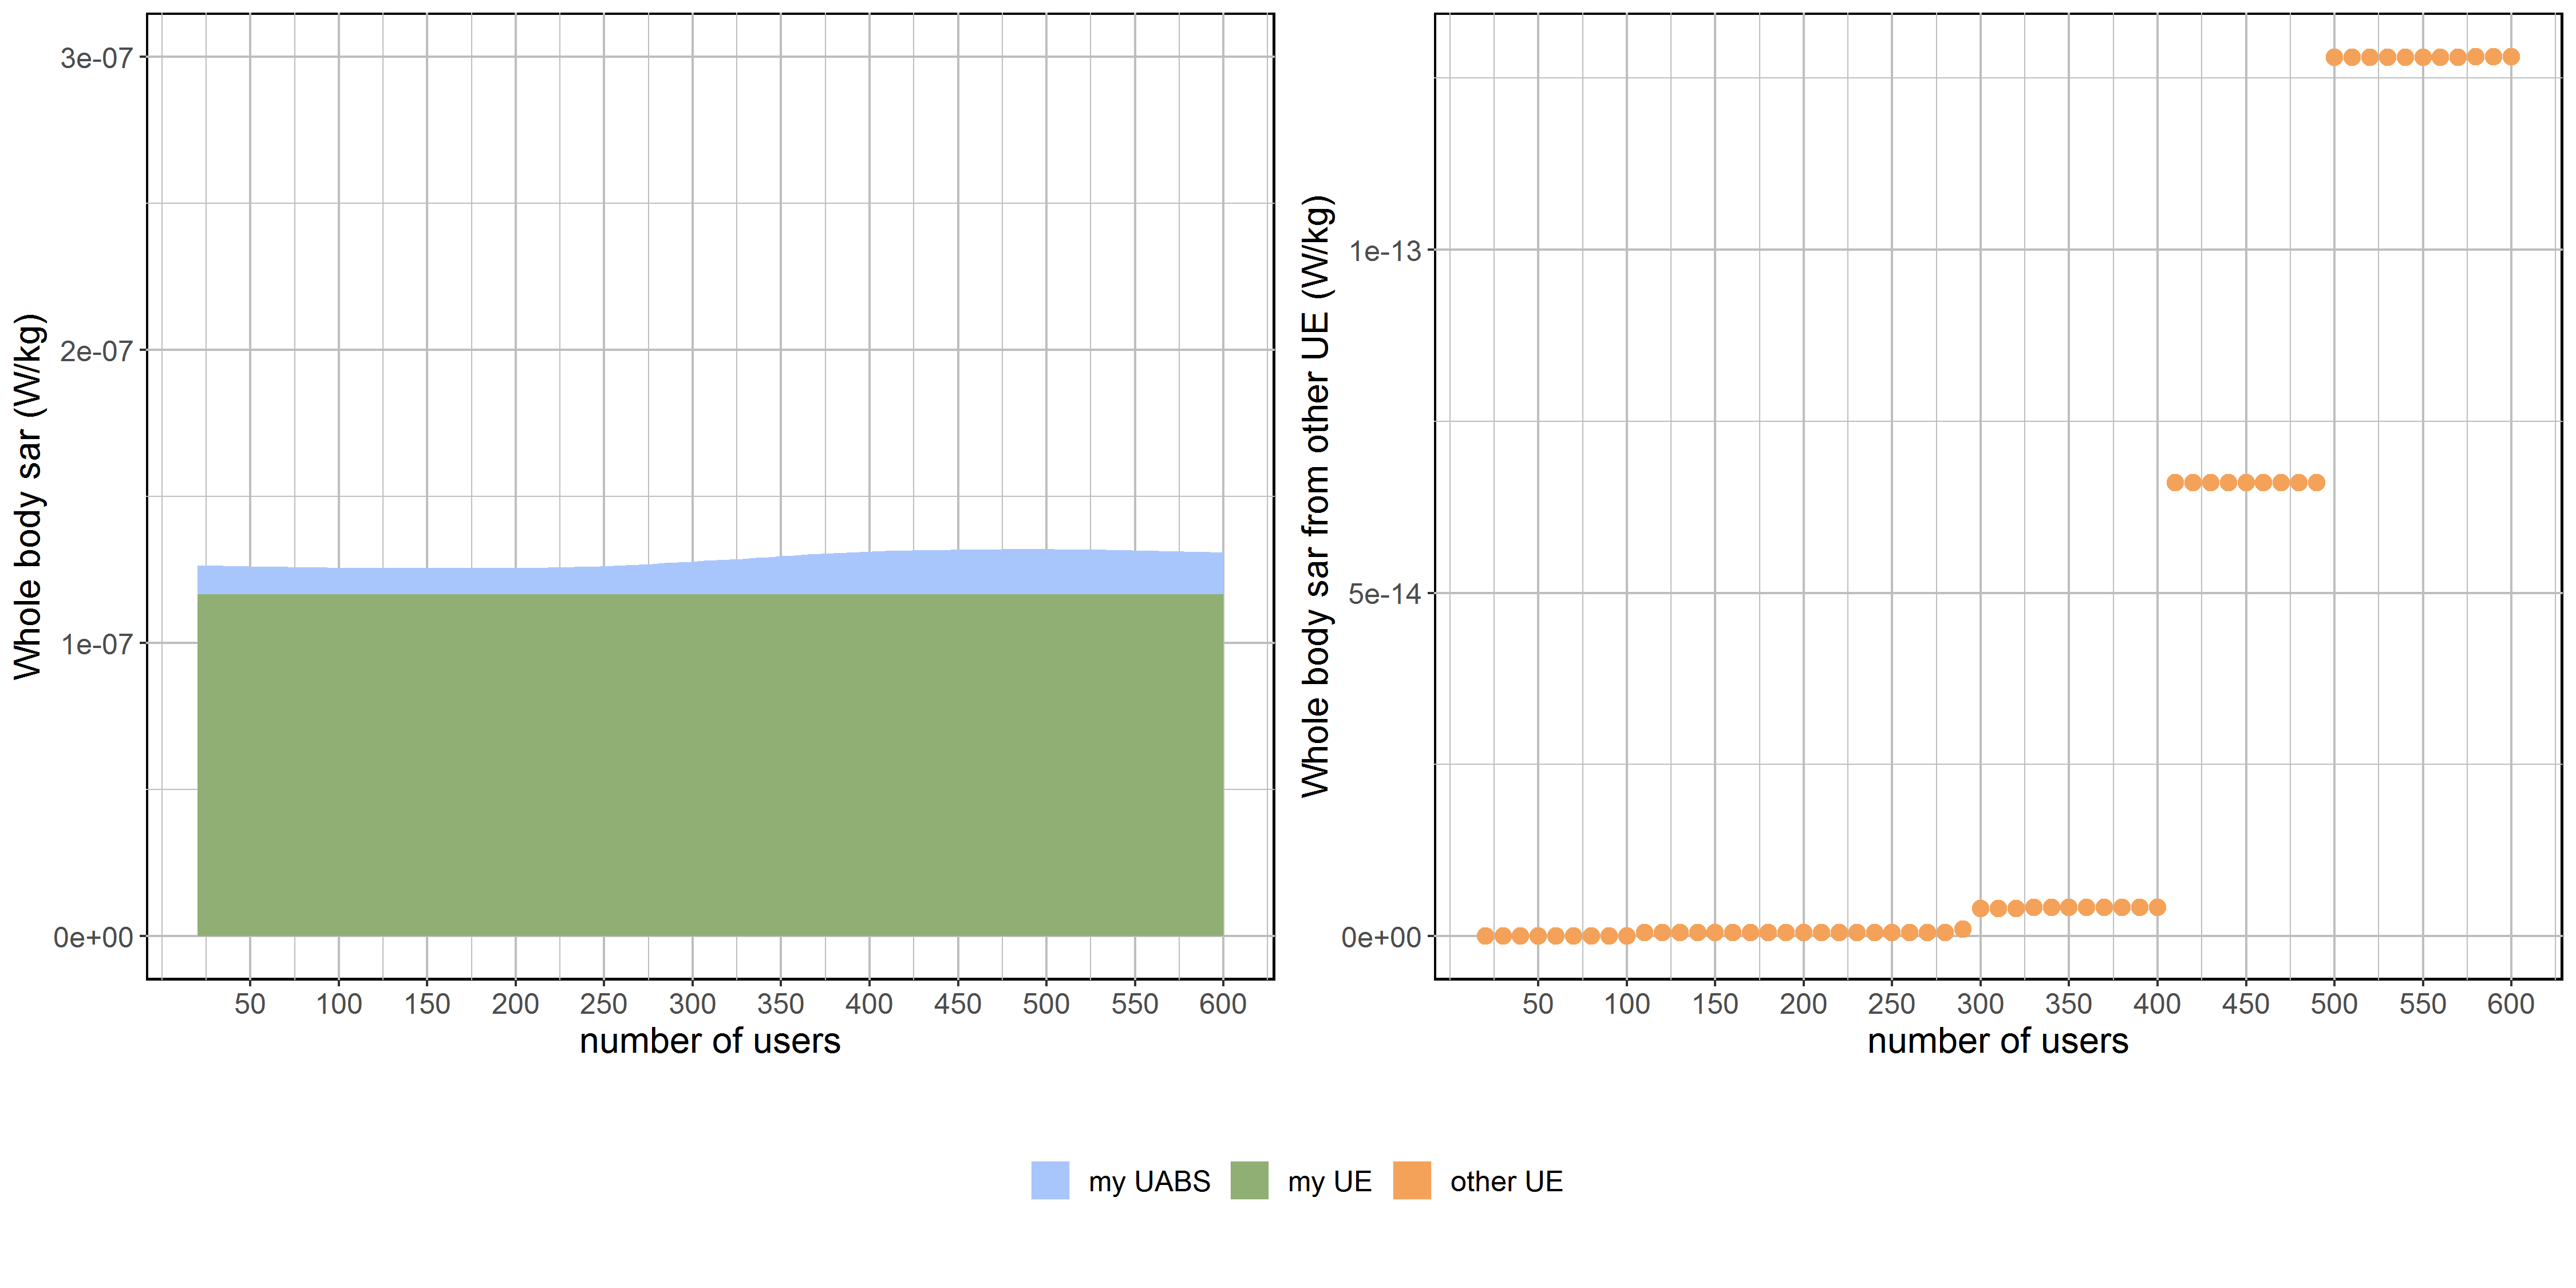
\includegraphics[width=\textwidth/6*5]{../results/s2/uvsulsarcentralUser.png}
  \caption{SAR-values for the user who is directly beneath the only UABS available.}
  \label{fig:uvsulsarcentralUsers}
\end{figure}

Scenario 1 already showed that the \gls{SAR} from the user's own device is only influenced by the flying height. 
The flying height for this experiment is fixed and the \gls{UL} \gls{SAR} from his device should therefore be also a constant. 
A hypothesis that is confirmed by figure \ref{fig:uvsulsarcentralUsers}.
The \gls{SAR} from the \gls{UABS} experience a slight  increase. When the population grows, more users become available 
of which some will spawn near the central user. The \gls{UABS} will likely decide to cover these user  as well as visible in figure \ref{fig:connectionMap}.
These user might have a slightly 
worse path loss because of obstructing buildings or somewhat bigger distance. The \gls{UABS} reacts to this by increasing 
his power consumption causing an increase in the \gls{DL} \gls{SAR} for the central user.

The far-field radiation from \gls{UE} is very low as mentioned before and is therefore not visible in figure \ref{fig:connectionMap} 
on the left and is therefore illustrated in a separate char on the right. 
It shows that the \gls{SAR}  from other \gls{UE} indeed increases. This is normal 
behaviour considering that more and more people become available around the central user of which some will be connected to the \gls{UABS}
and therefore also emitting radiation.

\begin{figure}[!htb]
\minipage{0.50\textwidth}
  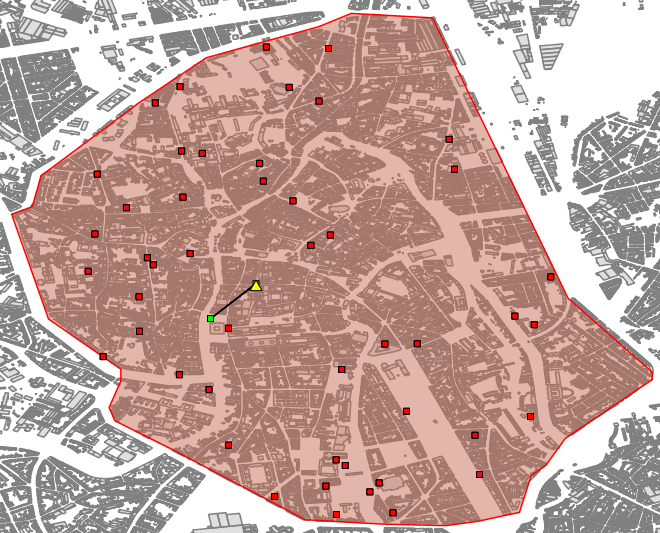
\includegraphics[width=\linewidth]{../images/connectionsMap50Users.png}
\endminipage\hfill
\minipage{0.50\textwidth}%
  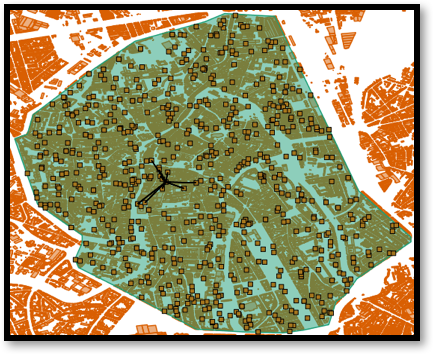
\includegraphics[width=\linewidth]{../images/connectionsMap600Users.png}
\endminipage
  \caption{Overview of which users are connected to the \gls{UABS}. The map on the left is for 50 active users while the map on the right is with 600 active users.}
  \label{fig:connectionMap}
\end{figure}
%%%%%%%%%%%%%%%%%%%%%%%%%%%%%%%%%%%%%%%%%%%%%%%%%%%%%%%%%%%%%%%%%%%%%%%%%%%%%%%%%%%%%%%%%%%%%%%%%%%%%%%%%%%%%s
\section{Scenario 3: Unlimited \gls{UAV}s}
\label{s3}

This scenario has just like the previous scenario much more users in the network 
and investigates the same cases which includes the variable flying height and the variable number of  users.
The only difference is that the restriction of only one \gls{UABS}s is dropped.

\subsection{Influence of the Flying Altitude}
\label{S3A}

The first case of this scenario examines how the network behaves for various flying heights and a fixed number of 224 users.
Scenario 2 already explained that when only one \gls{UAV} is available, a power consumption optimized network won’t result in a low 
powered network. In this scenario, there is no limitation on the number of \gls{UAV}s and the network remains thus unaltered after the decision 
algorithm is done. Figure \ref{fig:s3a_dlAndPc} clearly proves that the different optimization strategies work as intended.
Power consumption optimized networks have indeed a lower power consumption but therefore results in higher electromagnetic radiation.
On the other hand, an exposure optimized network will reduce the electromagnetic exposure by using more \gls{UAV}s and thence also increasing the network's power consumption.
This conclusion was already made  in \cite{J1} and is supported by these results.

\begin{figure}[h!]
  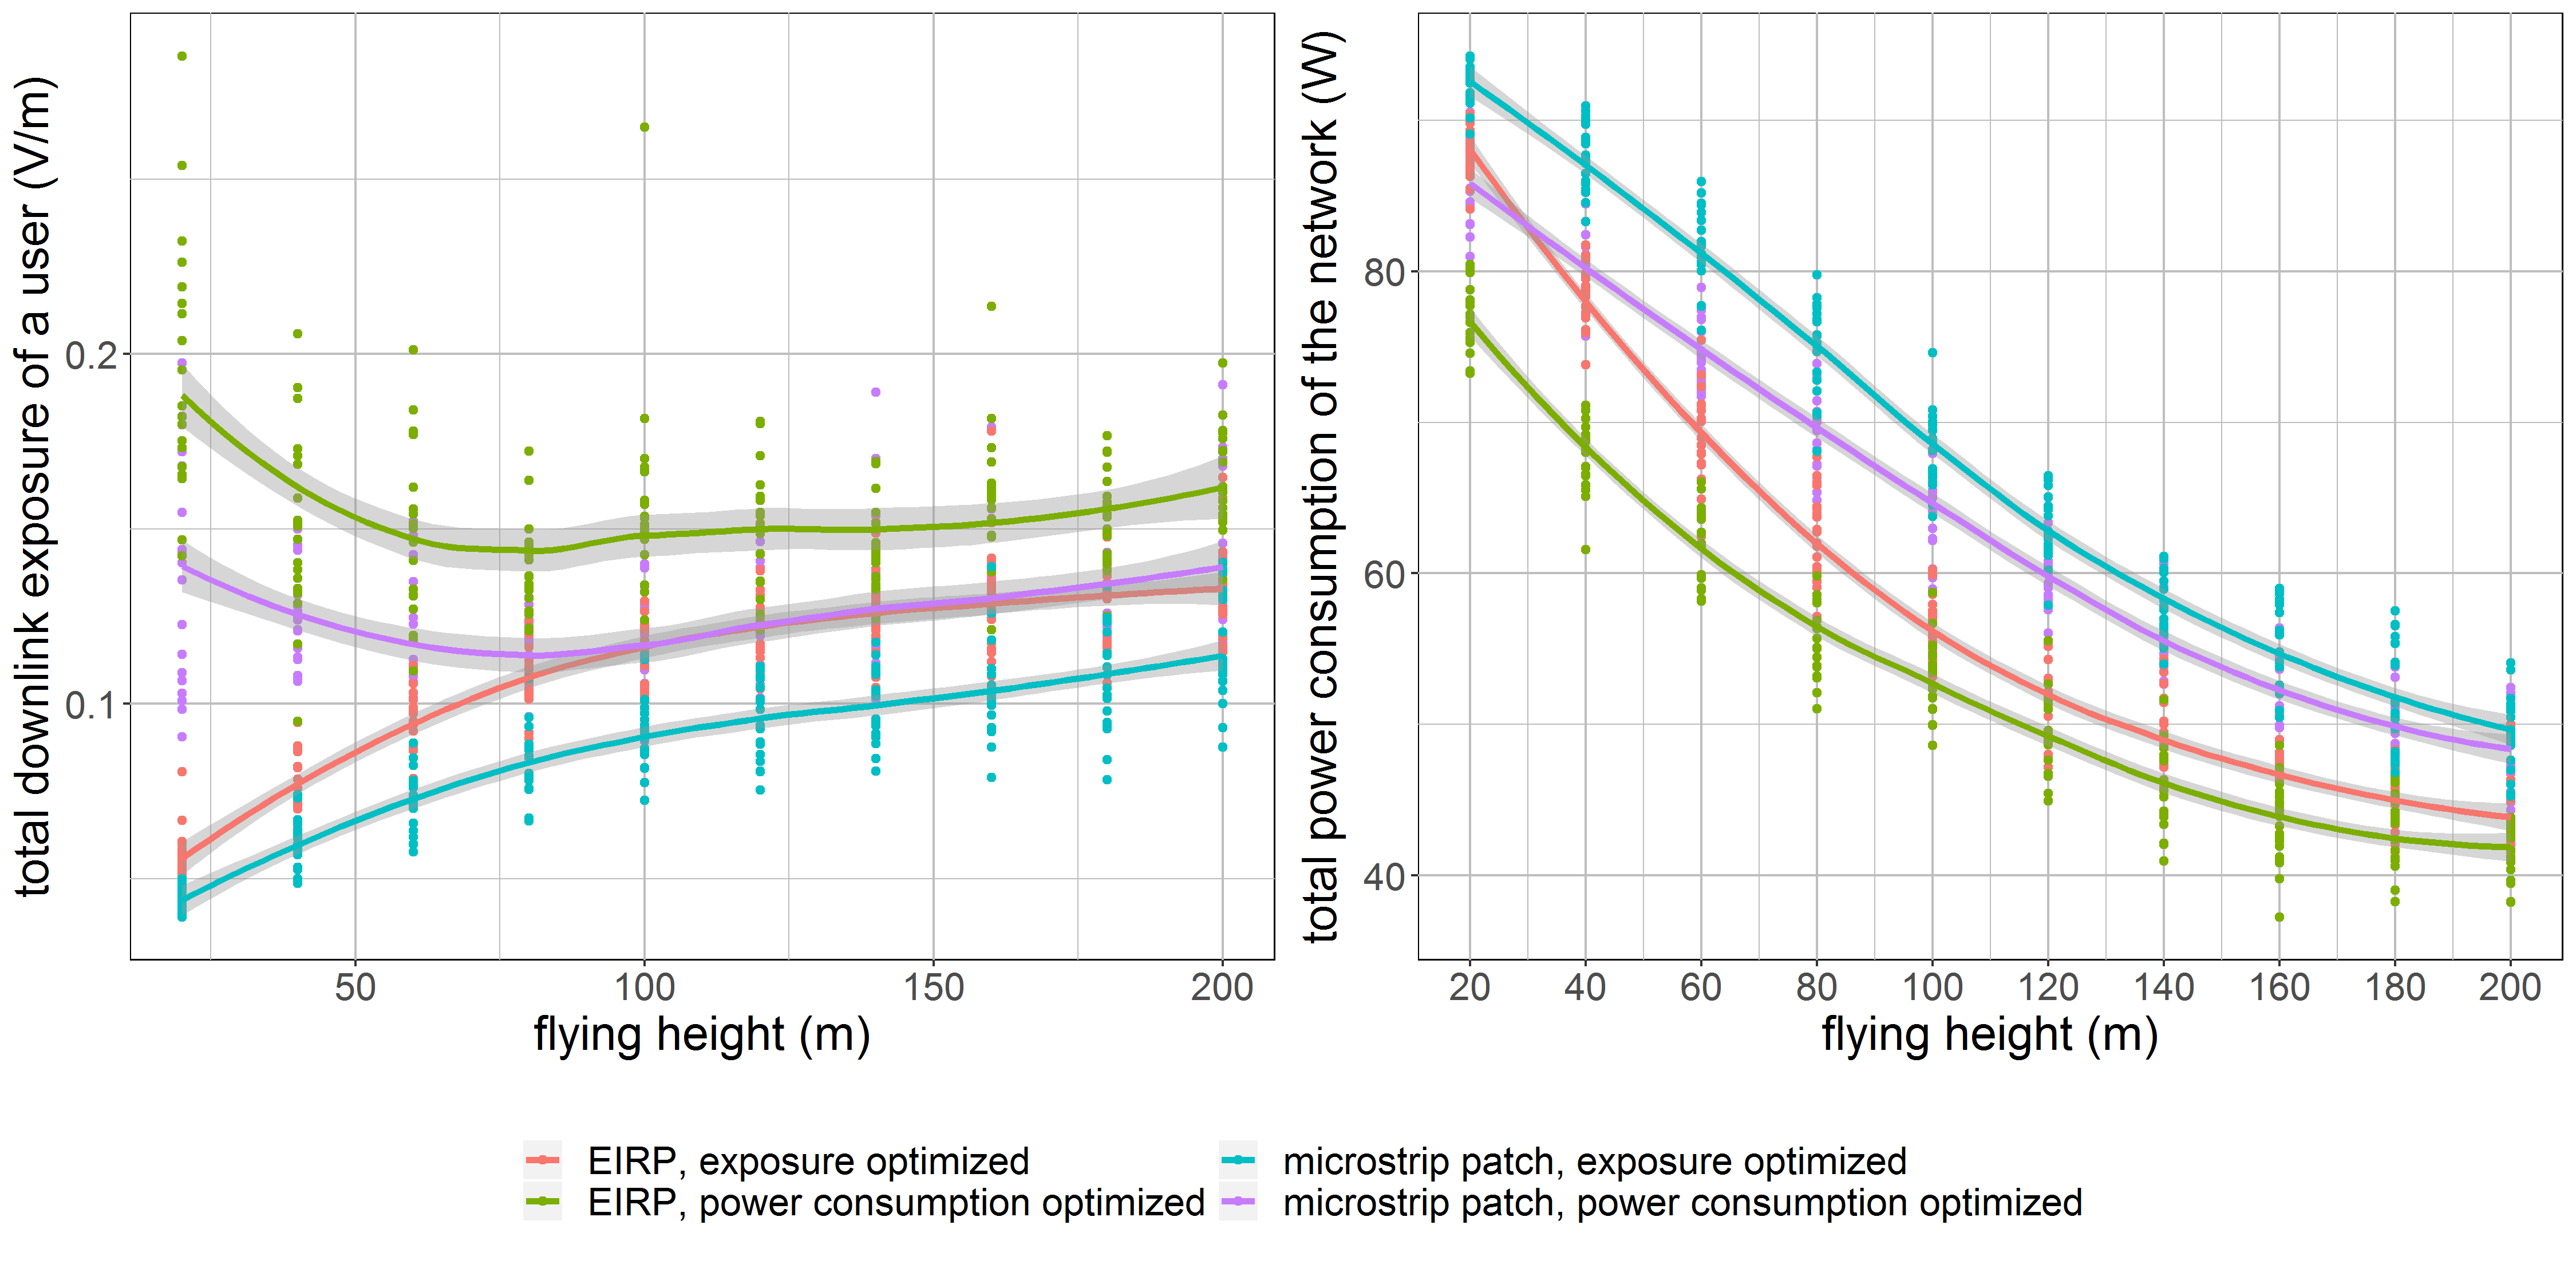
\includegraphics[width=\textwidth]{../results/s3/fhvsdlAndPc.png}
  \caption{The influence of the flying height on the downlink electromagnetic radiation of the average user.. This graph shows the percentage of covered users by one \gls{UAV} for different flying heights.}
  \label{fig:s3a_dlAndPc}
\end{figure}

Figure \ref{fig:s3a_dlAndPc}  shows that the number of \gls{UAV}s required decreases when the flying altitude becomes higher. A behaviour which was also determined in \cite{J2}.
At a low flying altitude, users in an exposure optimized network experience significantly lower exposure-values compared to a power consumption optimized network.
The exposure in a power consumption  optimized network starts high and 
decreases while an exposure optimized network behaves the opposite. This difference becomes less 
around 70 metres.
This can be explained when looking at figure \ref{fig:s3a_numDronesAndCov}.
At a flying height of 20 metres, the exposure optimized network has on average 220 to 224 \gls{UABS}s. That is (almost) one \gls{UABS} for each user
so it's logical that the electromagnetic exposure is very low.
The number of \gls{UAV}s in a power consumption optimized network is much less in order 
to save energy but figure \ref{fig:s3a_numDronesAndCov} shows on the  left the same percentage of coverage for this flying altitude.
So these \gls{UAV}s will try to cover users much further away and some of these connections will even be more worsened by obstructing buildings.
Because of this, users who are close and in \gls{LOS} will experience much higher electromagnetic radiation.
This path loss reduces when the \gls{UABS}s start to fly higher then the average  building and therefore exposure decreases.
Not only the power consumption optimized networks profit from higher flying altitudes, also the exposure optimized network does. For only a little bit 
more electromagnetic exposure, much less \gls{UAV}s are required.

\begin{figure}[]
  \includegraphics[width=\textwidth]{../results/s3/fhvsnum\gls{UAV}sAndCov.png}
  \caption{This graph shows how much \gls{UAV}s are required for different flying heights while trying to achieve a 100\% coverage.}
  \label{fig:s3a_numDronesAndCov}
\end{figure}

Both  \ref{fig:s3a_dlAndPc} and \ref{fig:s3a_numDronesAndCov}  show that the network profits from increasing the flying altitude. 
Not only less \gls{UAV}s are needed but also the power consumption is lower. Both can be explained by the lower path loss when \gls{UABS}s fly higher.

Scenario 1 already proved that with low flying \gls{UAV}s, the main source of electromagnetic radiation are \gls{UABS}s. 
This changed around 80 meters where \gls{UL} electromagnetic radiation of the \gls{UE}
exceeds \gls{DL} radiation in order to still be able to reach the high flying \gls{UABS}s. 
When looking at the different individual sources in \ref{fig:s3a_fourSourcesMatrix}, we see 
that \gls{UL} \gls{SAR} is logarithmic increasing despite the fact that figure \ref{fig:s1_fhsar} showed that the  \gls{UL} \gls{SAR} 
increases exponentially. This was however deducted with only one user is present in the network as opposed to this scenario 
where 224 users are present. The covered users will still behave like in scenario 1 but much more users are uncovered (fig. \ref{fig:s3a_numDronesAndCov}) 
which decreases the average \gls{SAR}. 
In conclusion, the average  \gls{UL} \gls{SAR}  won't increase as fast as the \gls{UL} \gls{SAR} of 
an individual that is covered.

\begin{figure}[]
  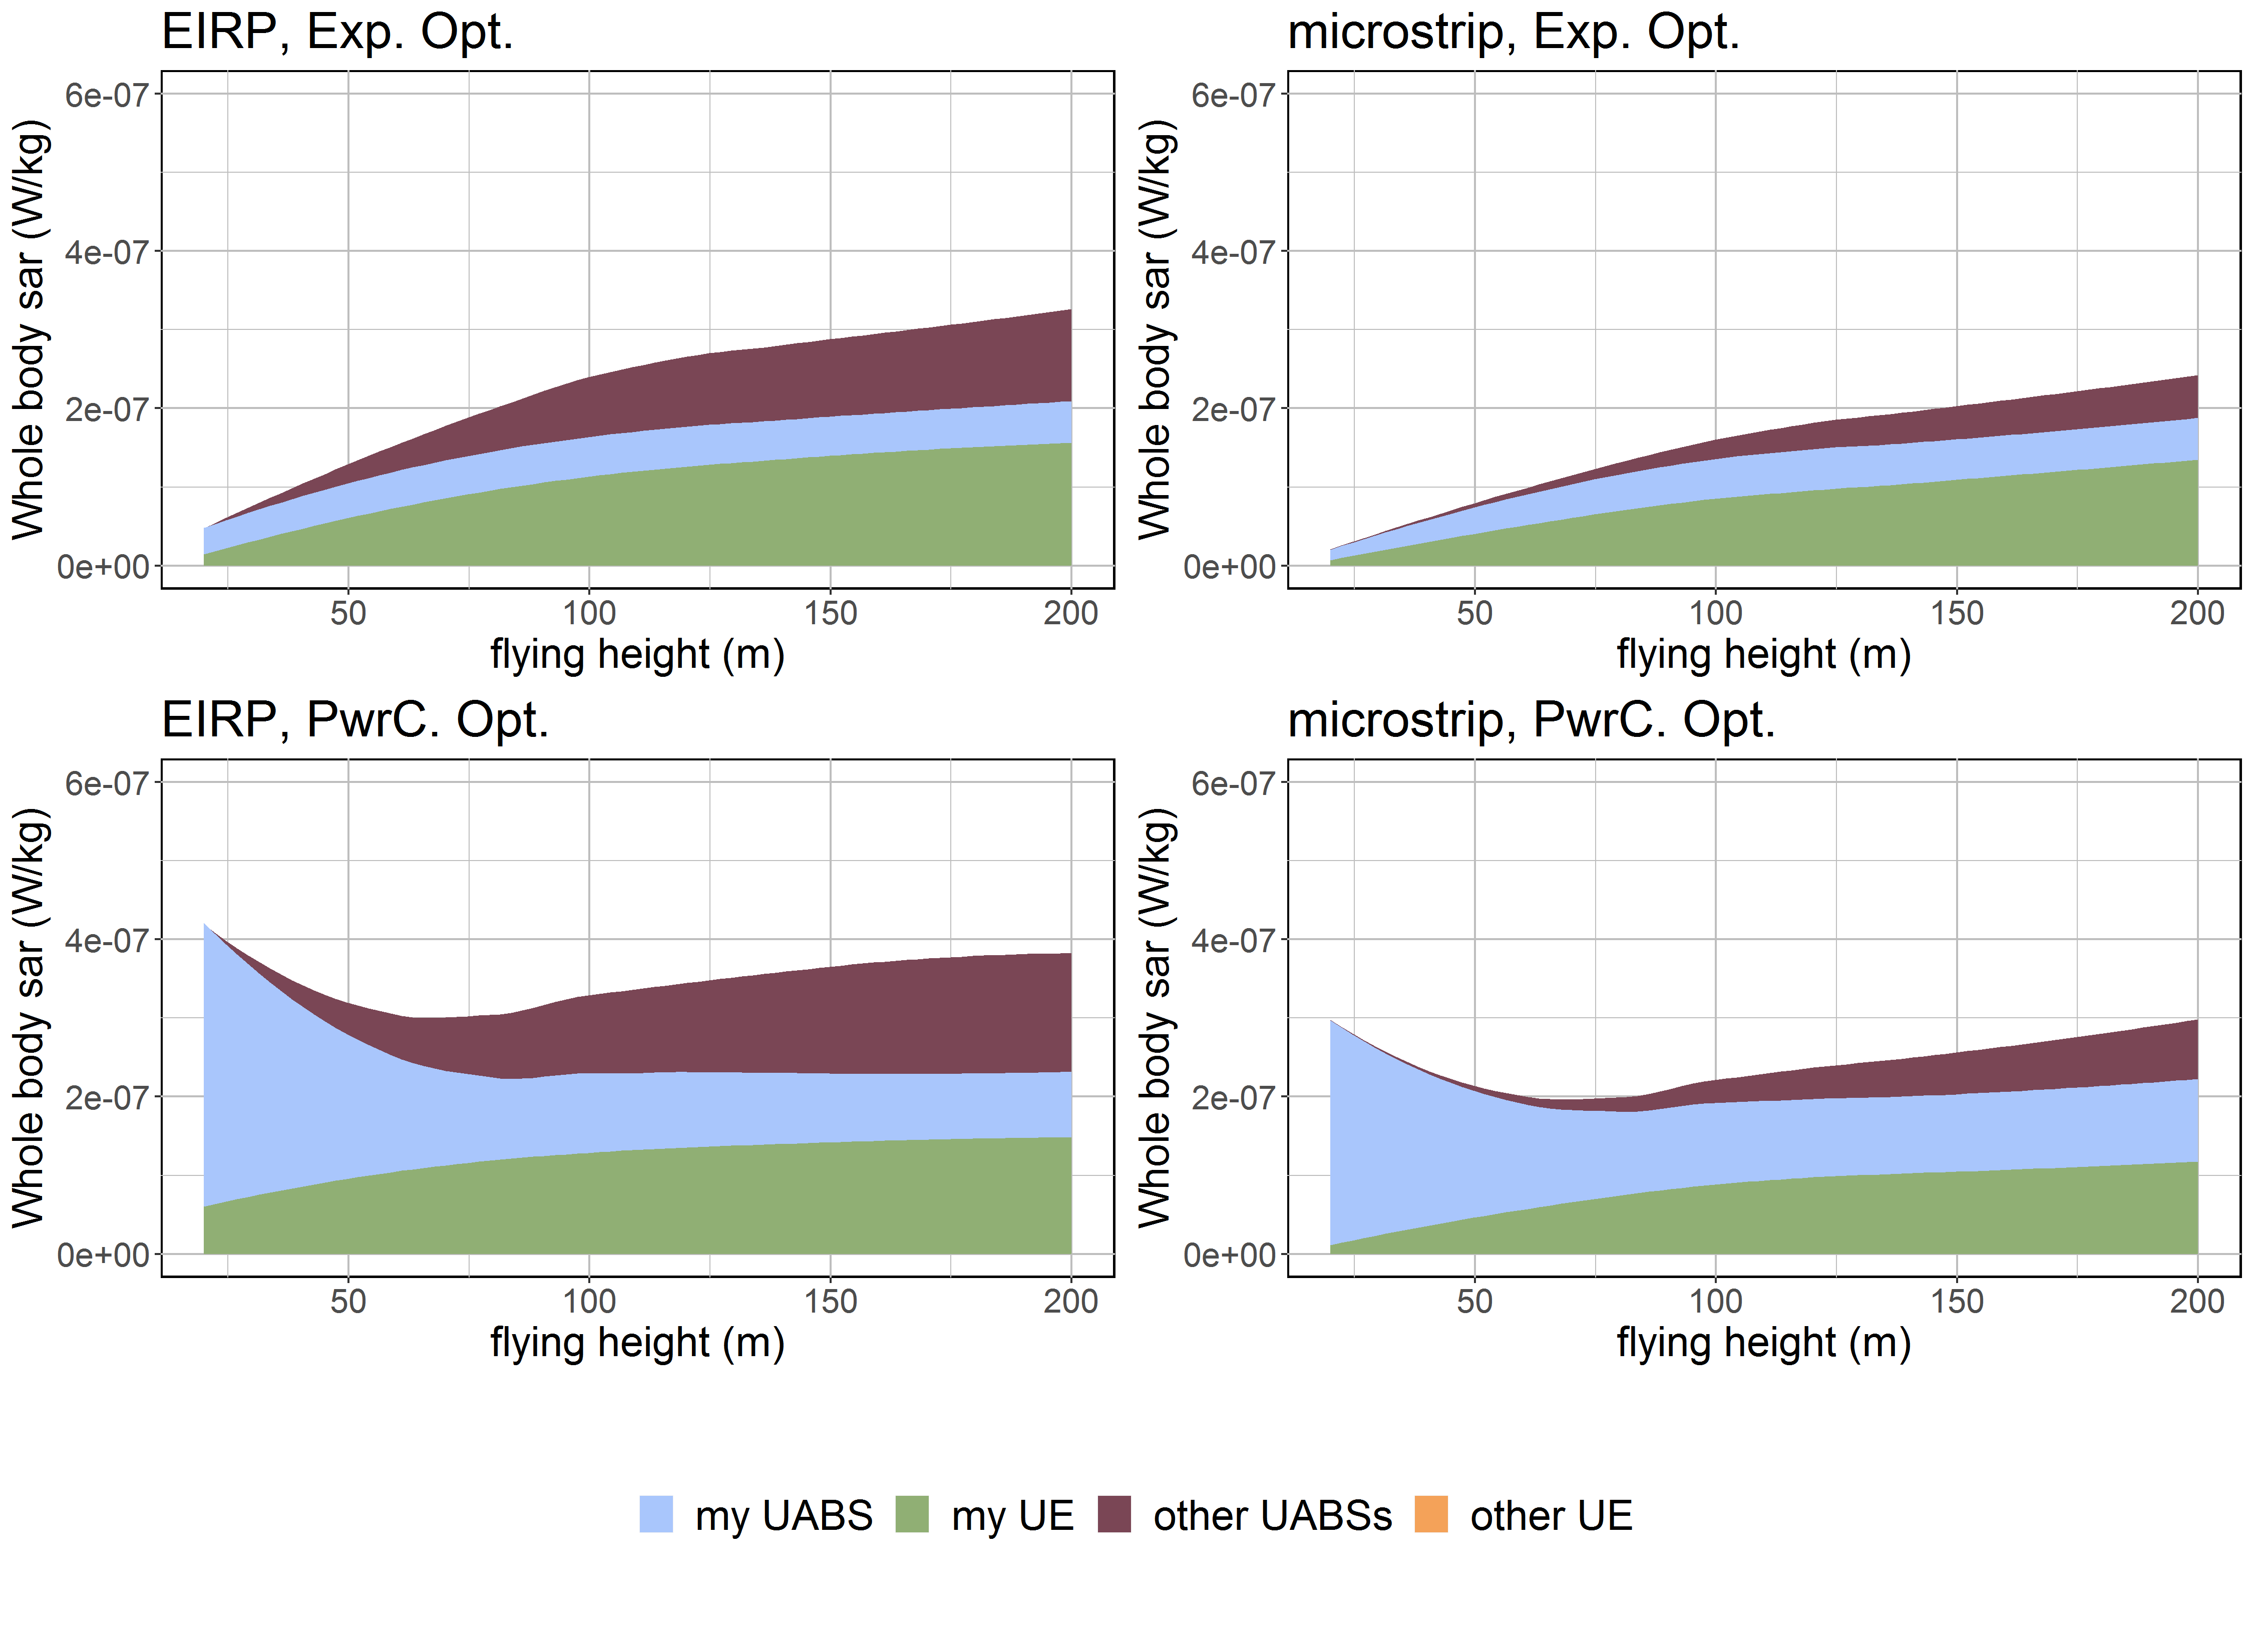
\includegraphics[width=\textwidth]{../results/s3/fhFourSources.png}
  \caption{Each chart shows the total SAR to which the average user is exposed. ``My UABS" stands for the UABS that is serving our average user while ``other UABSs'' stand for 
  all other UABSs to which that user is exposed to but not served by. ``Other" UE refer the exposure from all mobile devices that does not belong that user.}
  \label{fig:s3a_fourSourcesMatrix}
\end{figure}

We can see from \ref{fig:s3a_fourSourcesMatrix} that once the buildings level out (around 70 to 80 metres), the SAR from the serving \gls{UABS} remain 
more or less constant. A behaviour that was already determined in `scenario 1' and `scenario 2: experiment \ref{fig:uvsulsarcentralUsers}'. 

When looking at the exposure from `other \gls{UABS}s', we see an increase in electromagnetic radiation at higher 
flying altitudes.
Also here will the lower path loss from  less obstructing buildings be the reason.
The figures from \ref{fig:s3a_fourSourcesMatrix} further also clearly show that this increase 
in electromagnetic radiation will be less for a microstrip patch antenna. The reason behind this is that energy 
will be more focussed towards the ground and there is less sideways radiation because of attenuation.


%%%%%%%%%%%%%%%%%%%%%%%%%%%%%%%%%%%%%%%%%%%%%%%%%%%%%%%%%%%%%%%%%%%%%%%%%%%%%
\FloatBarrier
\subsection{Influence of the Number of Users}
\label{S3B}

The last case of scenario 3 investigates a variable number of users for a fixed flying height of 100 m. There is no 
restriction on the number of available \gls{UAV}s just like in the previous case meaning that there are at most 
as much \gls{UAV}s as users in the network. The correct behaviour of the decision algorithm became already clear in the previous subsection \ref{S3A} but is also
confirmed by this case.
Figure \ref{fig:s3b_num\gls{UAV}sAndCov} shows on the left how the tool tries to reach a 100\% coverage. The tool reaches this goal 
better for larger populations. The difference remains however very little. The tool also requires more \gls{UAV}s for these large 
populations. An expected behaviour  when looking at scenario \ref{s2b} where, with only one \gls{UABS} available, the percentage of covered users decreases for these larger populations.
 The difference in optimization strategy is very little for small amounts of people but increases very fast. Further, \ref{fig:s3b_dlAndPC} shows an increase 
 in exposure for larger populations because more \gls{UAV}s come with these larger populations and more 
 exposure comes with more \gls{UAV}s as visible in \ref{fig:s3b_num\gls{UAV}sAndCov}.

\begin{figure}[h!]
  \includegraphics[width=\textwidth]{../results/s3/uvsnum\gls{UAV}sAndCov.png}
  \caption{This graph shows how much \gls{UAV}s are required for different flying heights while trying to achieve a 100\% coverage.}
  \label{fig:s3b_num\gls{UAV}sAndCov}
\end{figure}

In a scenario with 600 active users, a clear difference is noticeable between the four configurations. 
For instance, an EIRP power consumption optimized 
network requires the least amount of \gls{UAV}s (Figure \ref{fig:s3b_num\gls{UAV}sAndCov} on the right). This is logical when looking at figure \ref{fig:s3b_dlAndPC} where \gls{UAV}s in such a configuration cause the highest amount of 
electromagnetic radiation. This behaviour was already discussed in subsection \ref{s2b}. 

On the complete opposite, we have a microstrip patch antenna in an exposure optimized network. 
This strategy prioritize the minimization of electromagnetic exposure. In addition, a microstrip antenna has a much more limited range.
Therefore, much more 
\gls{UAV}s are required in order to reach 100\% coverage (Figure \ref{fig:s3b_num\gls{UAV}sAndCov}) and therefore requires much more energy 
to power all the \gls{UAV}s (Figure \ref{fig:s3b_num\gls{UAV}sAndCov} on the right).

So scenario 3 learns that a power consumption optimized network indeed result in less \gls{UAV}s and less 
 power consumption of the entire network. 
At the same time, scenario 2 showed that the active \gls{UABS}s have a higher individual power consumption.
We can therefore state that a power consumption optimized network will reduce it's total power consumption by
using a few high powered \gls{UAV}s.

Likewise for an exposure optimized network, we can conclude that the network has indeed a lower electromagnetic exposure but the power consumption 
of the entire network is much higher. In scenario 2 became already clear that the active \gls{UABS}s have a low power consumption in order to 
guarantee a low electromagnetic exposure towards the users.
We can conclude that an exposure optimized network will reduce the exposure of an individual by 
using a lot low powered \gls{UAV}s.

\begin{figure}[h!]
  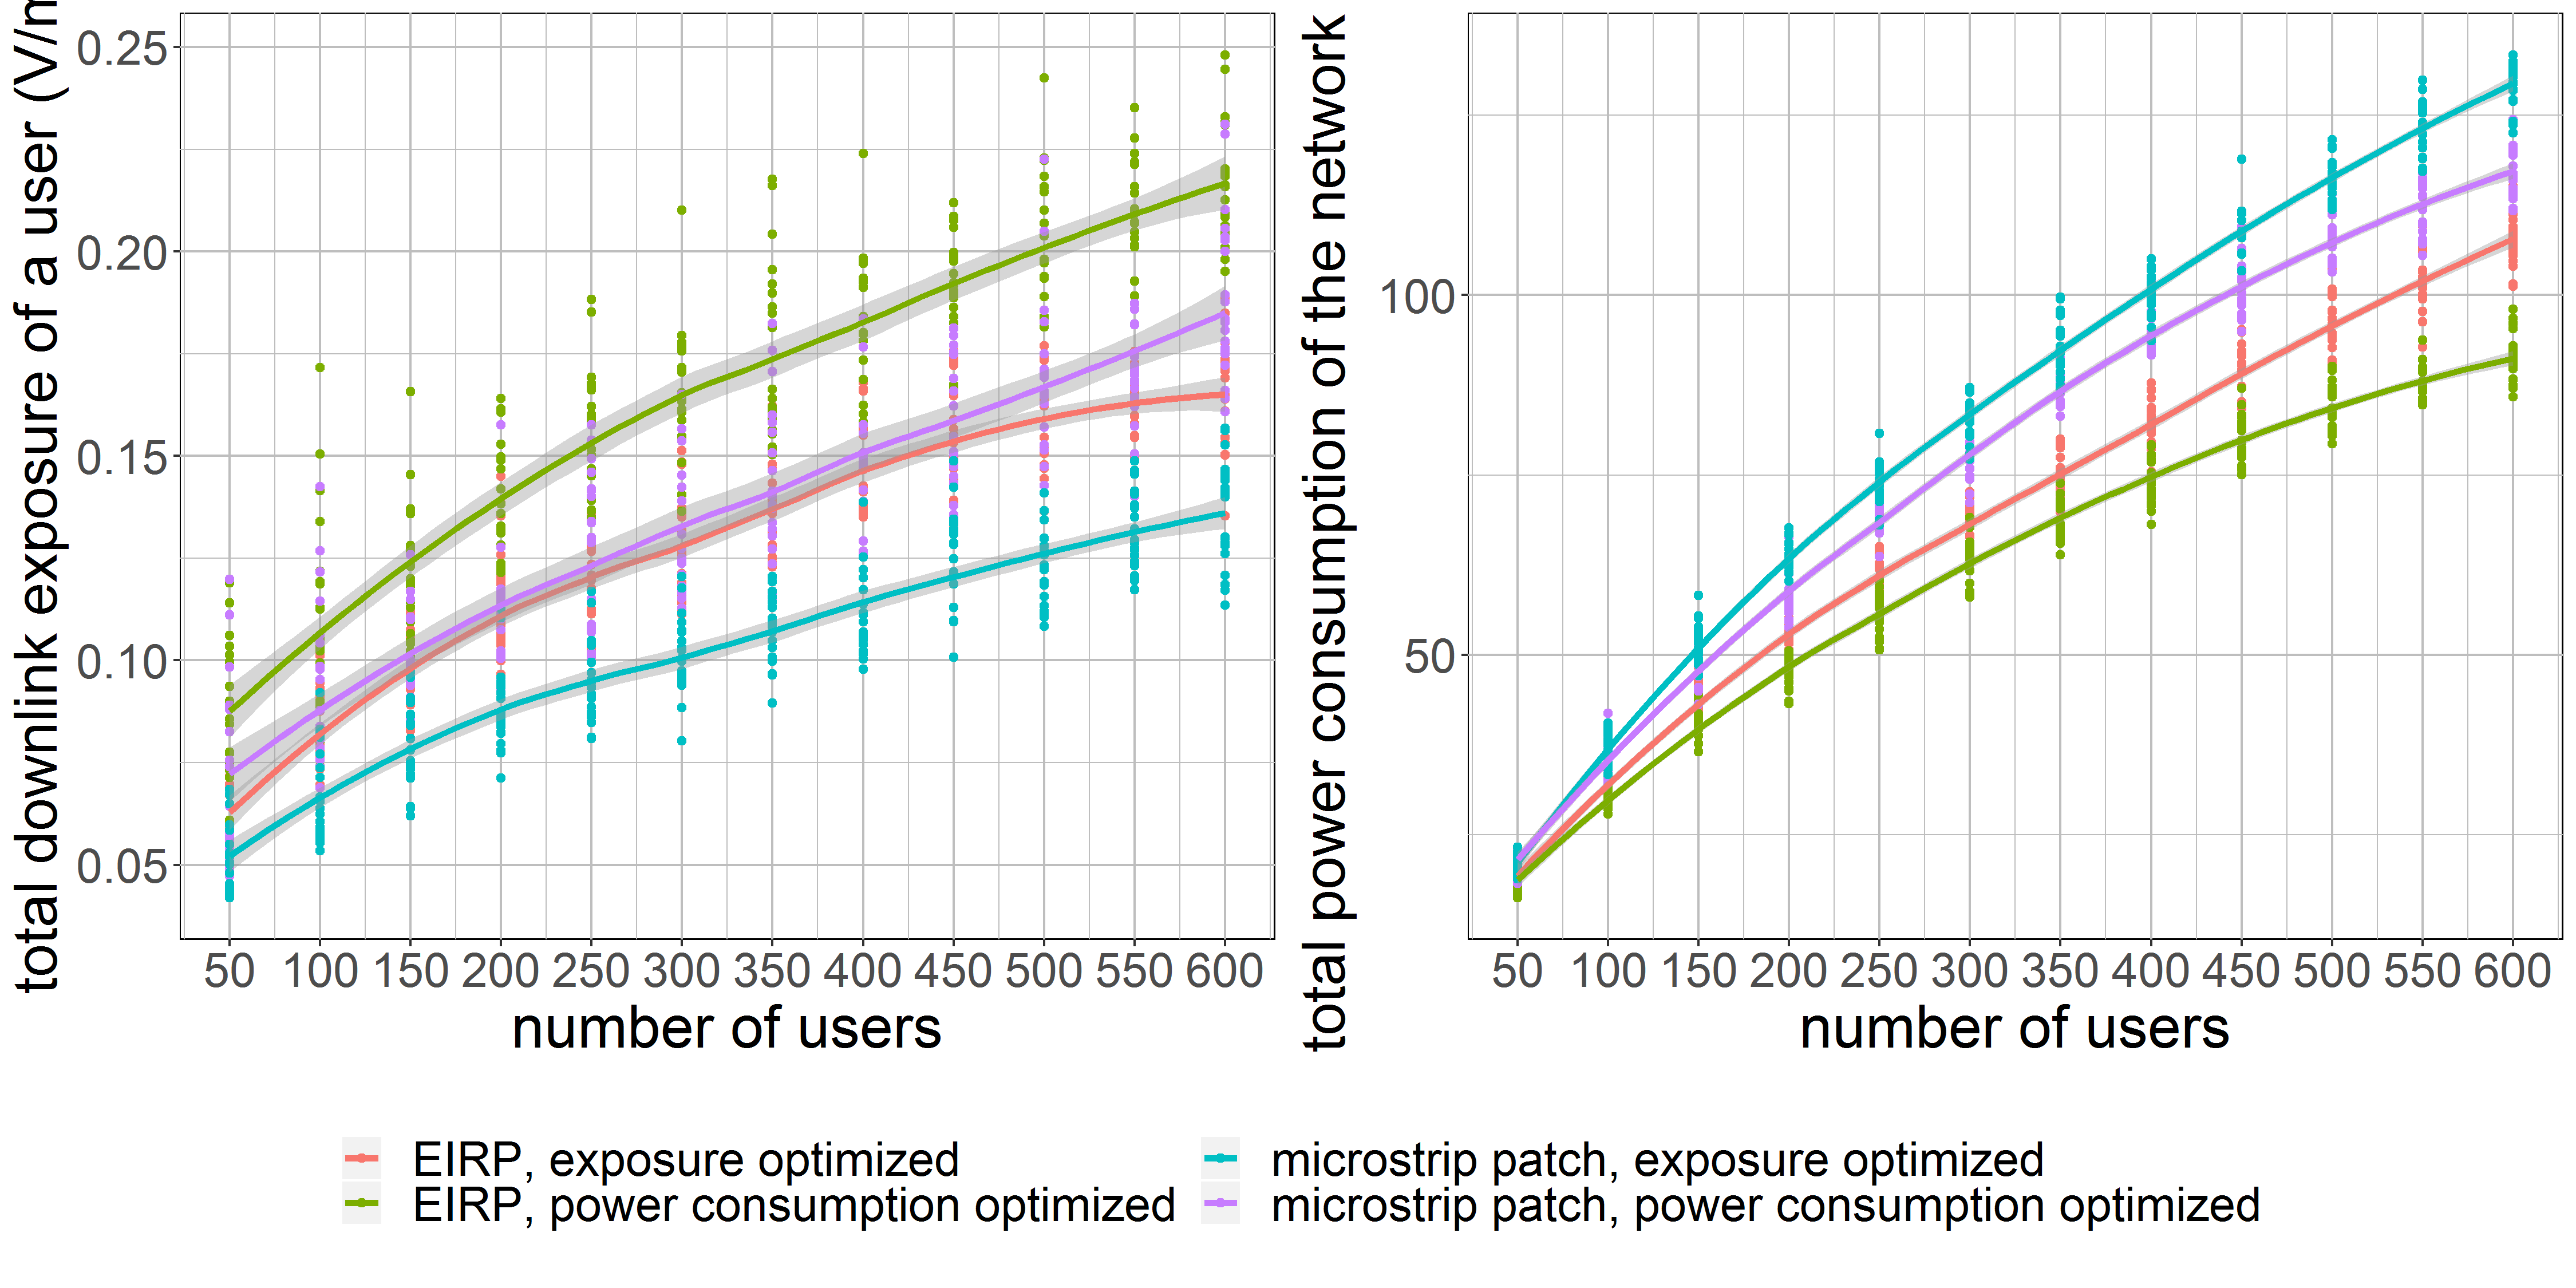
\includegraphics[width=\textwidth]{../results/s3/uvsdlAndPc.png}
  \caption{The influence of the flying height on the downlink electromagnetic radiation of the average user.}
  \label{fig:s3b_dlAndPC}
\end{figure}

When looking at the different contributions to the total \gls{SAR} in figure \ref{fig:s3b_fourSourcesMatrix}, 
we see that the weighted average 
\gls{SAR} from the users own device remains constant. The flying altitude is always the same so the
 \gls{UE} will, on average, radiate at the same intensity for all simulations.
 Further, the \gls{DL} \gls{SAR} from the serving \gls{UABS} is also almost constant  because the \gls{UABS} flies at 100 metres which is
above the average building. There is thus a \gls{LOS} between the \gls{UABS} and most of his connected users.
The only \gls{SAR} value that increases are the \gls{DL} \gls{SAR} from other \gls{UABS}s and the \gls{UL} \gls{SAR} from other \gls{UE}. 
When more users come online, also more \gls{UAV}s will be radiating. Moreover, there is very little path loss because the flying height is above the average building.

\begin{figure}[h!]
  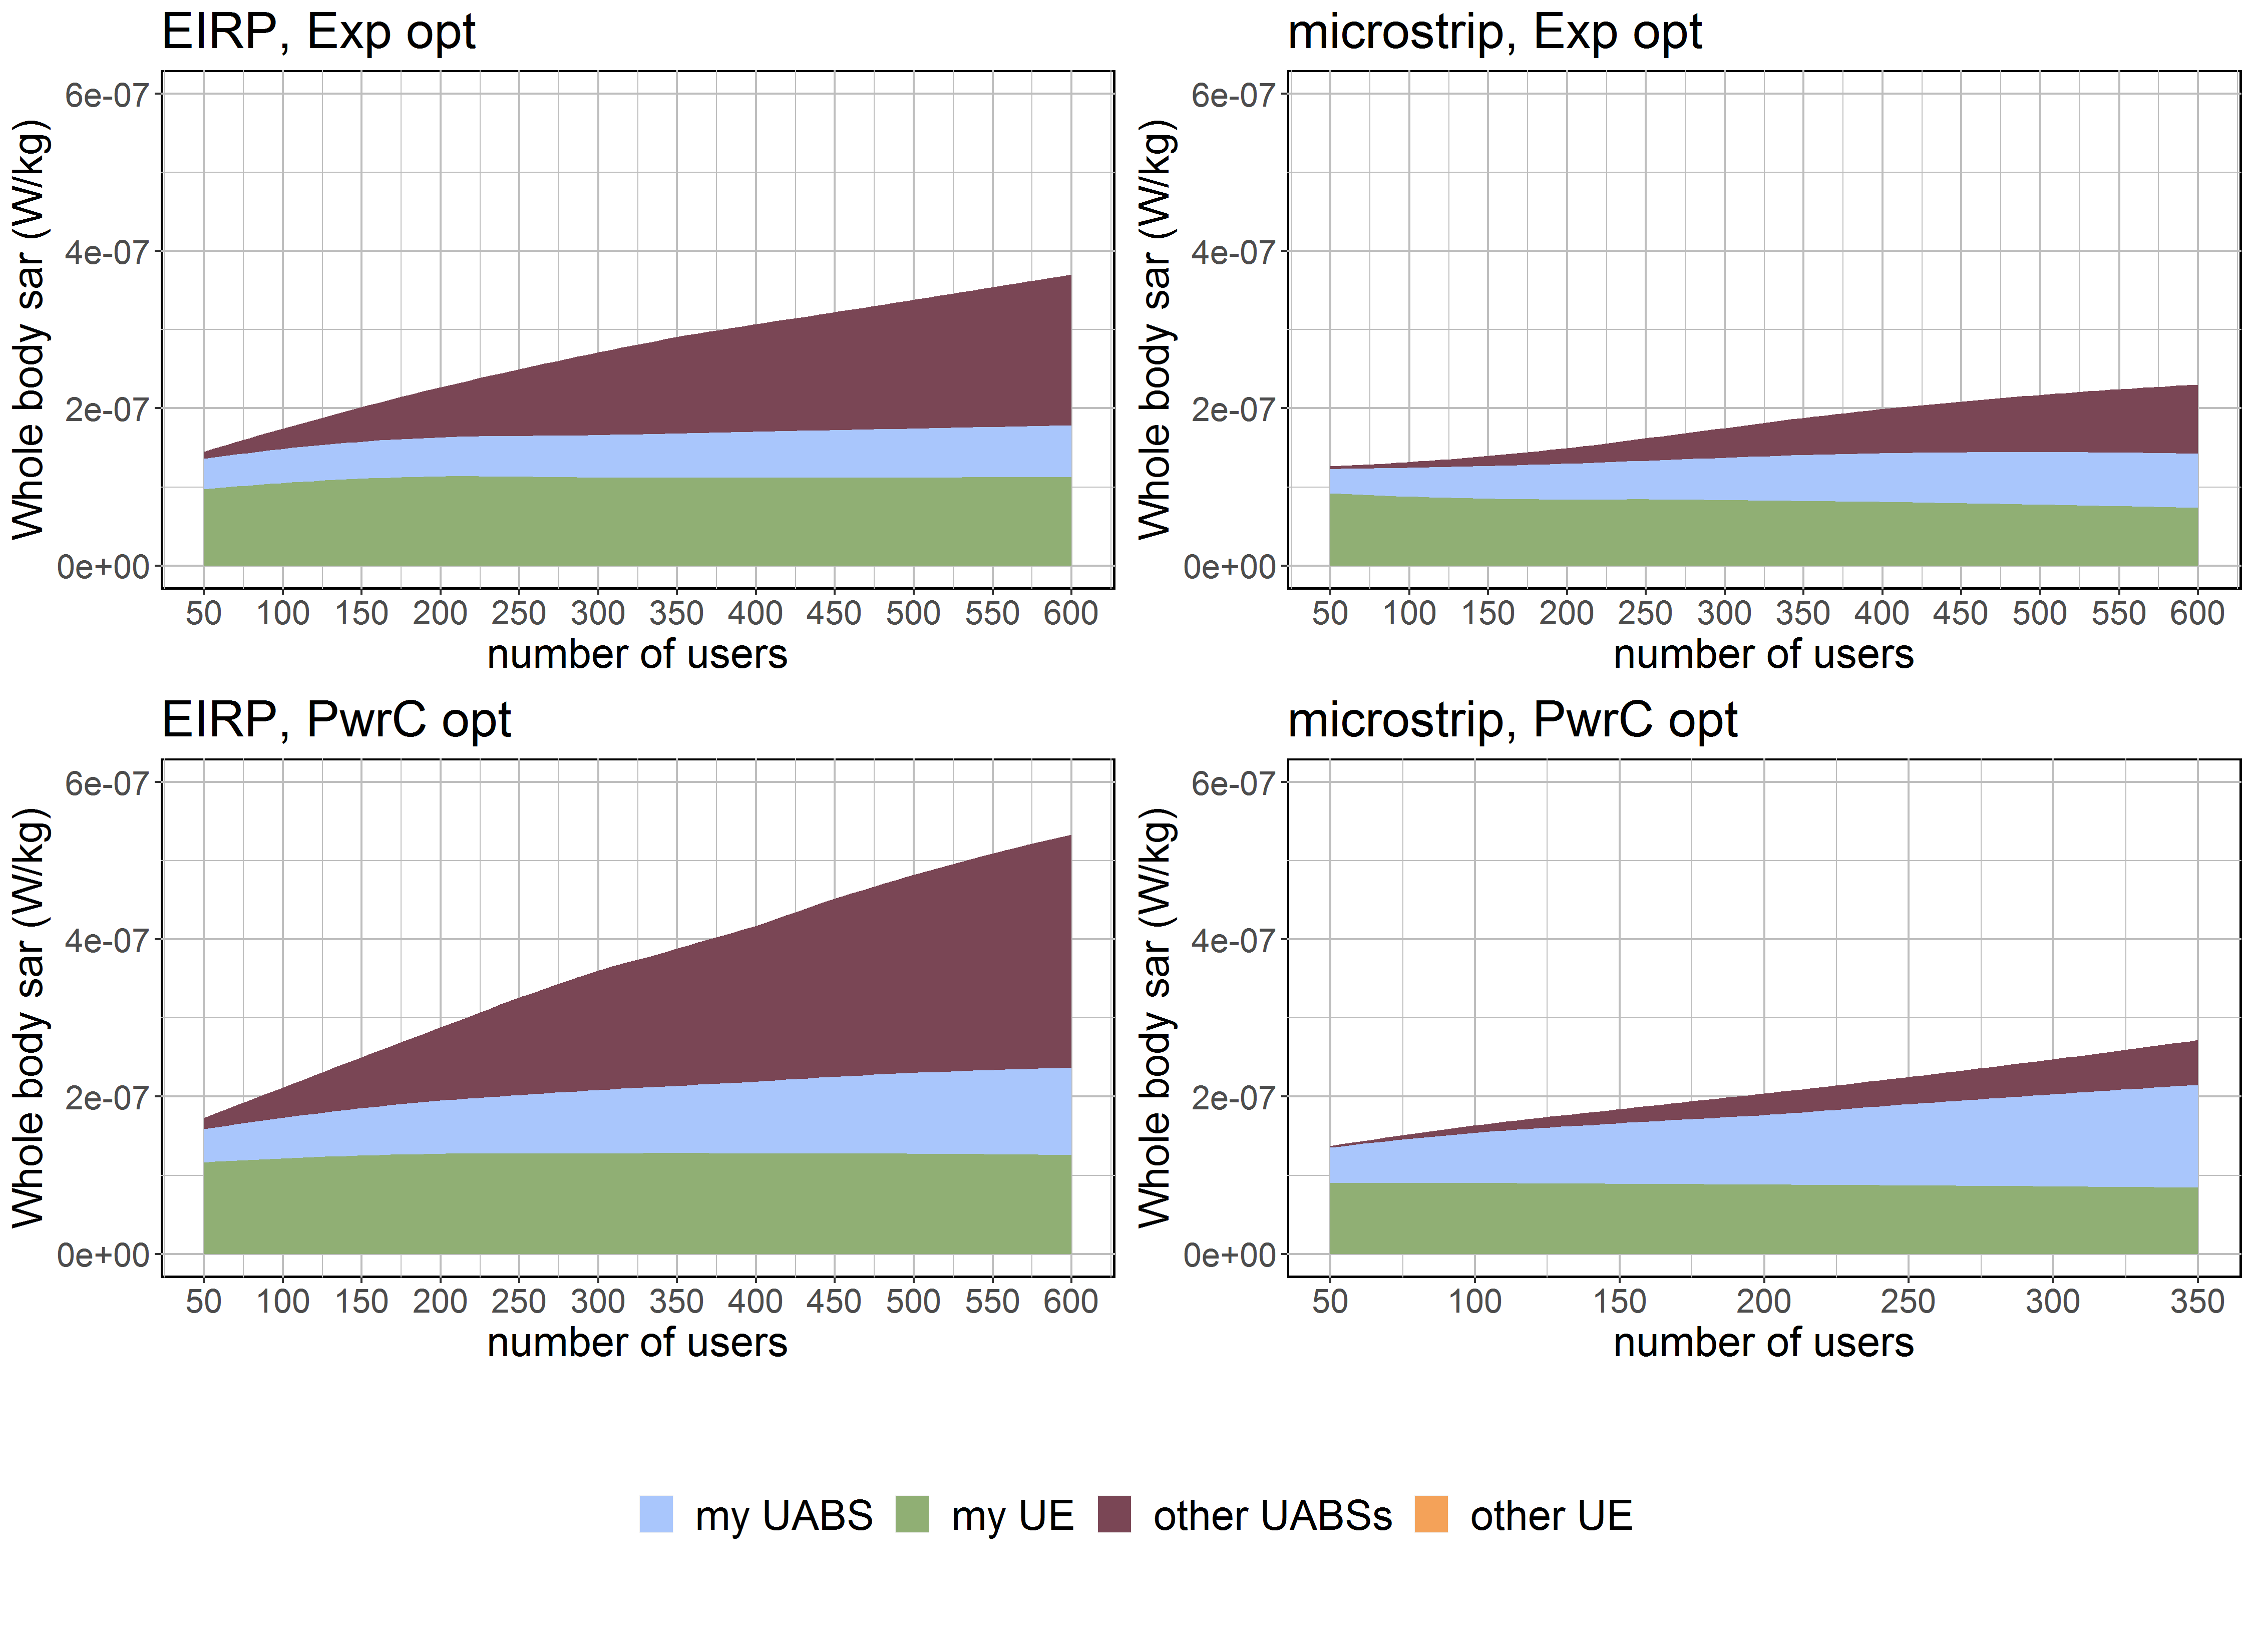
\includegraphics[width=\textwidth]{../results/s3/uFourSources.png}
  \caption{Each chart shows the total SAR to which the average user is exposed. ``My UABS" stands for the UABS that is serving our average user while ``other UABSs'' stand for 
  all other UABSs to which that user is exposed to but not served by. ``Other" UE refer the exposure from all mobile devices that does not belong that user.}
  \label{fig:s3b_fourSourcesMatrix}
\end{figure}
\chapter{Conclusions}
\label{chap:conclusions}

The following section presents the conclusion where the impact of the flying height and users population in a \gls{UAV}-aided network
is investigated by examining electromagnetic exposure and power consumption. Also, optimization techniques towards both evaluation 
parameters have been applied and two different antenna types have been considered.
All conclusions are based on the default configuration with a flying height of 100 metres and 224 active users to cover.
The other parameters are described in table \ref{table:defaultconf}.

\section{Conclusion}

%How can a UABS network be optimized to minimize global exposure or overall power consumption? 
Literature showed that a network can be optimized towards either the power consumption of the entire network 
or the electromagnetic exposure of the average user using a fitness function. This is because the power required to activate a new 
base station is much higher than for raising the electromagnetic radiation and therefore increasing its range \cite{J1}.
The fitness function was originally applied for fixed transmission towers but can also be used 
for \gls{UABS}s as this research shows.
However, the fitness function should be used with care considering that \gls{UABS}s can be placed anywhere as opposed to 
the transmission towers from \cite{J1} who have a predetermined position.  
For default networks, the electromagnetic field radiation from a
power consumption optimized network can be reduced up to 23\% for \gls{isotropicradiator}s and 30\% for microstrip patch antennae 
by optimizing towards electromagnetic exposure. Doing so, decreases the range of the \gls{UABS} and much more \gls{UABS}s will be needed. 
Therefore, exposure optimized networks will, on average, use 18 drones more than power consumption optimized networks
and require therefore 5 $W$ more energy.
A power consumption optimized network on the other hand will try to limit the number of drones 
in order to save energy.
 So as a rule of thumb: an exposure optimized network will result in a lot of low powered devices (increasing the overall power consumption)
while a power consumption optimized network results in a few high powered devices (increasing the exposure of the average user).
The authors from \cite{J17_kuehn2019modelling} confirm this by stating that smaller cells will reduce electromagnetic radiation. 
If the goal is to remain in the air for a longer period of time, an exposure optimized network is recommended because the power consumption of 
an individual \gls{UABS} is lower.
On the other hand, a power consumption optimized network is cheaper because less drones are involved.
Moreover, the results show that the electromagnetic radiation in a power consumption optimized network (with high powered \gls{UABS}s)
is far below the thresholds enforced by the Flemish government with more than a hundred thousandth of the maximal allowed whole body \gls{SAR}.

\definecolor{c_myuabs}{HTML}{A9C6FC}
\definecolor{c_otheruabs}{HTML}{7A4655}
\definecolor{c_myue}{HTML}{90AF74}
\definecolor{c_otherue}{HTML}{F4A259}

\begin{figure}
\begin{tikzpicture}
\pgfplotsset{
        show sum on top/.style={
            /pgfplots/scatter/@post marker code/.append code={%
                \node[
                    at={(normalized axis cs:%
                            \pgfkeysvalueof{/data point/x},%
                            \pgfkeysvalueof{/data point/y})%
                    },
                    anchor=south,
                ]
                {\pgfmathprintnumber{\pgfkeysvalueof{/data point/y}}};
            },
        },
    }
  \begin{axis}[
    title={SAR for default configuration},
    ylabel={Whole body SAR (nW/kg)},
    xlabel={Configurations},
    height=7cm, width=\textwidth,
    legend cell align={left},
    ybar stacked, ymin=0,  
    bar width=10mm,
    %symbolic x coords={a,b,c,d},
    symbolic x coords={EIRP PwrC Opt, EIRP Exp Opt, Microstrip PwrC Opt, Microstrip Exp Opt},
    xtick=data,
    nodes near coords, 
    nodes near coords align={anchor=center},%Move values in bar
    every node near coord/.style={
    },
  ]
  %myUABS
  \addplot [fill=c_myuabs!50] coordinates {
({EIRP PwrC Opt},73)
({EIRP Exp Opt},50)
({Microstrip PwrC Opt},98)
({Microstrip Exp Opt},45)};
  %other uabs
  \addplot [fill=c_otheruabs!50,text=black] coordinates {
({EIRP PwrC Opt},105)
({EIRP Exp Opt},70)
({Microstrip PwrC Opt},30)
({Microstrip Exp Opt},25)
};
%myue
  \addplot [fill=c_myue!50,show sum on top] coordinates {
({EIRP PwrC Opt},127)
({EIRP Exp Opt},115)
({Microstrip PwrC Opt},87)
({Microstrip Exp Opt},85)
};
%other ue
  \addplot [fill=c_otherue!50,show sum on top] coordinates {
({EIRP PwrC Opt},0)
({EIRP Exp Opt},0)
({Microstrip PwrC Opt},0)
({Microstrip Exp Opt},0)
};
  \legend{my UABS,other UABSs,my UE,other UE}
\end{axis}
\end{tikzpicture}
\caption{The contribution of each source towards the total \acs{SAR} for each considered configuration. 
The values are achieved with default values.}
\label{fig:tabel}
\end{figure}


%	How does the network behave differently after the introduction of a realistic antenna?
A directional microstrip patch antenna is introduced because it gives several advantages compared to omnidirectional antennae.
Directional antennae are able to focus their energy there where it is needed, namely towards the ground. Microstrip patch antennae 
further benefit from their thin and lightweight design. The performance 
of this directional microstrip patch antenna has been compared to a 
fictional \gls{isotropicradiator}.
This \gls{isotropicradiator} has higher exposure and coverage for less power compared to a microstrip patch antenna.
For a default network, a microstrip patch antenna can reduce between 30\% and 34\% electromagnetic exposure 
from an \gls{isotropicradiator}. Doing so will require around 24 drones extra and therefore increasing the power consumption with 11 $W$.
The fact that an \gls{isotropicradiator} has higher electromagnetic exposure for less power  is due to the absence of 
attenuation and can hypothetically be compared to an antenna with a very big aperture angle.
A microstrip patch antenna with a more limited aperture angle of \ang{90} requires more resources but 
causes less sideways radiation. So the exposure from other \gls{UABS}s will also be less.

\begin{figure}[hb!]
\centering
  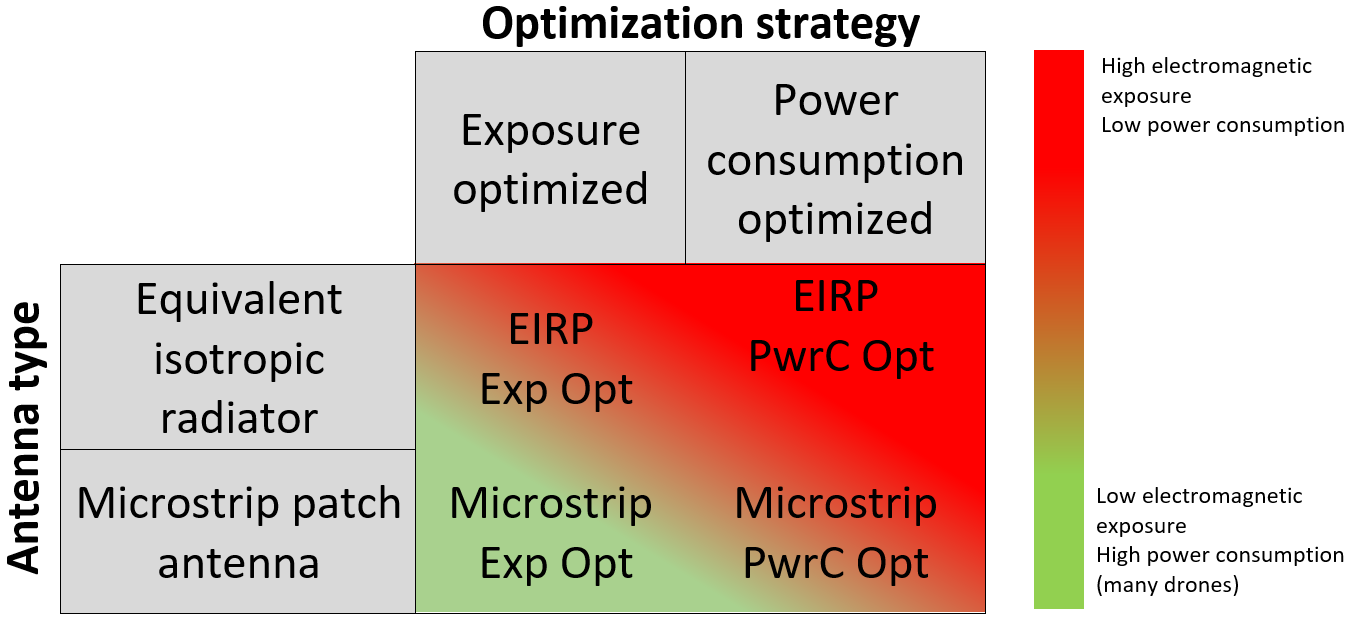
\includegraphics[width=0.8\textwidth]{../images/fourCasesMatrixSol.png}
  \caption{Matrix with the four possible configurations, colour-coded based on the results.}
  \label{fig:resultIllustration}
\end{figure}

Figure \ref{fig:resultIllustration} shows an overview based on the results from the two optimization strategies and the two types of antenna.
Remarkable is that an \gls{EIRP} exposure optimized network behaves very similar to a microstrip power consumption optimized network.
Therefore, the microstrip patch antenna in a power consumption optimized network is recommended. 
The microstrip patch antenna will generate less electromagnetic radiation by design and
 the power consumption optimization reduces the number of required drones and power. A microstrip patch antenna with an aperture 
 angle of \ang{90} is considered as a good solution but if budget is more limited, an antenna with a larger aperture angle 
 would further reduce cost without interfering with the Flemish legislation regarding electromagnetic exposure.


%What is the contribution of each source towards the total electromagnetic exposure?
Figure \ref{fig:pie} gives
an overview of the contribution of \gls{SAR} in percentage to the total 
exposure for a default network. The values have been averaged over all four considered configurations. 
The user's main source of exposure is clearly the user's own device which contributes 52\% of the total experienced exposure.
A conclusion that was also made by the authors of \cite{J17_kuehn2019modelling}
where a 5G network is simulated and by the authors from  \cite{J10.1.1} 
where a \gls{GSM} and \gls{UMTS} network is simulated. Further, in \cite{J10.1.1} is also concluded that,
thanks to power control, the electromagnetic radiation from the mobile phone 
comes really close to the exposure from the \gls{UABS}. 
Also this is confirmed by the results. Figure \ref{fig:pie} shows that the electromagnetic exposure 
from all \gls{UABS}s together covers the remaining 48\% of which 15 \% is from the serving UABS. 
The electromagnetic
 exposure from devices belonging to other people can be ignored compared to the much higher electromagnetic exposure from the other sources
 and contributes only 0.0001\%. It is important to notice that a rather low \gls{pusch} value is used in equation \ref{eq:powerUE} for determining the 
 \gls{UL} radiation and it is believed that a higher value will have a major effect on the \gls{SAR} from the user's own 
 device but also from neighbouring devices. Investigating this parameter is however out of scope and could be addressed in a future work.


\def\angle{0}
\def\radius{3}
\def\cyclelist{{"c_myue","c_otheruabs","c_myuabs","c_otherue"}}
\newcount\cyclecount \cyclecount=-1
\newcount\ind \ind=-1
\begin{figure}[h!]
\centering
 \resizebox {!} {5.5cm} {
\begin{tikzpicture}[nodes = {font=\sffamily}]
  \foreach \percent/\name in {
      52/ my UE,
      33/ other UABSs,
      15/ my UABS,
      0/ Other UE
    } {
      \ifx\percent\empty\else               % If \percent is empty, do nothing
        \global\advance\cyclecount by 1     % Advance cyclecount
        \global\advance\ind by 1            % Advance list index
        \ifnum3<\cyclecount                 % If cyclecount is larger than list
          \global\cyclecount=0              %   reset cyclecount and
          \global\ind=0                     %   reset list index
        \fi
        \pgfmathparse{\cyclelist[\the\ind]} % Get color from cycle list
        \edef\color{\pgfmathresult}         %   and store as \color
        % Draw angle and set labels
        \draw[fill={\color!50},draw={\color}] (0,0) -- (\angle:\radius)
          arc (\angle:\angle+\percent*3.6:\radius) -- cycle;
        \node at (\angle+0.5*\percent*3.6:0.7*\radius) {\percent\,\%};
        \node[pin=\angle+0.5*\percent*3.6:\name]
          at (\angle+0.5*\percent*3.6:\radius) {};
        \pgfmathparse{\angle+\percent*3.6}  % Advance angle
        \xdef\angle{\pgfmathresult}         %   and store in \angle
      \fi
    };
\end{tikzpicture}
 }
\caption{Contribution from each source towards the total SAR that is experienced by the weighted average user. 
The percentages are averaged over the four 
considered configurations.}
\label{fig:pie}
\end{figure}

%How does the \gls{UABS} flying height and number of users influence electromagnetic exposure and power consumption?
As last, the results confirm that the flying height and population size have a major influence on electromagnetic exposure and 
power consumption. It becomes clear that more \gls{UABS}s are required when the population size increases. 
This results in a higher power 
consumption and electromagnetic exposure. When the population increases from 50 to 600 users, 
the electromagnetic radiation increases between 80 and 130 $mV/m$ depending
on the configuration. The power consumption increases with 110 $W$ for all configurations. 
The main source that is influenced by the number of users is the \gls{SAR} from other UABSs with an increase between 1 and 3 $\mu W/kg$, depending on 
the configuration.
Further, increasing the flying altitude has a positive influence on the number of required drones which on their 
turn have a positive influence on power consumption. Increasing the flying altitude from 20 m to 200 m, decreases the number 
of required drones around 59\%. This decrease in number of \gls{UABS}s was also concluded in \cite{J2}.
Also authors from \cite{J17_kuehn2019modelling} made the conclusion that reduced path loss decreases electromagnetic exposure.
The electromagnetic radiation from the \gls{UABS}s remains more or less the same for flying altitudes between 80 and 200 metres. Most 
\gls{UABS}s are in \gls{LOS} and no more power will be used thanks to power control.
However, the electromagnetic radiation from the user's own device does increase in order to reach the high flying drones.
At around 80 metres, the exposure from the  user's device surpasses the exposure from the serving \gls{UABS}.
When more \gls{UABS}s are available in the network, electromagnetic exposure from other \gls{UABS} will increase as well 
because more \gls{UABS}s come into \gls{LOS}. Raising the flying altitude from 20 to 200 m will increase the \gls{SAR} from other 
\gls{UABS}s between 46 and 49 times when using an \gls{EIRP} antenna and between 70 and 85 times when using a microstrip patch antenna.
It is therefore concluded that raising the flying height has a positive influence on the number of 
\gls{UABS}s but is not unlimited since the total \gls{SAR} will increase as well.
When also considering the results from \cite{U1} where a flying altitude of  
80 metres is suggested for an optimal access and backhaul connectivity, a flying height 
of 80 metres is also here proposed for the city centre of Ghent.

\section{Summary}
The microstrip patch antenna with an aperture angle of \ang{90} is a suitable starting point for an antenna. 
This directional antenna focusses electromagnetic radiation where it is needed. Unwanted sideways radiation 
is therefore reduced by design.
The sufficiently large aperture angle covers enough users. The antenna is recommended to be deployed in a power consumption 
optimized network since less drones are required and therefore also less expensive.
The optimal flying height for the city centre of Ghent is believed to be situated at 80 metres since lower flying heights require much more \gls{UABS}s and
higher flying heights have a negative influence on the electromagnetic exposure.  

\section{Future work}

Despite the fact that many parameters have been examined, still some parameters require further investigations.
The \gls{pusch} value defines the minimal required signal strength received by the \gls{UABS} and still needs to be evaluated
for different values. Also, the exposure caused by backhaul links has not been evaluated yet.

The chosen microstrip patch antenna is solely based on literature and performing an excessive research to various 
types of radiation patterns is outside the scope of this master dissertation. It is expected that the radiation can 
further be improved by using microstrip patch antennae in more complex array-configurations. 

The tool provides support for any possible radiation pattern and applies this to any \gls{UABS}.
However, despite some minor changes, each \gls{UABS} can has its custom radiation pattern which makes 
3D beamforming possible. Therefore, electromagnetic exposure can be determined for base stations where MiMo
and massive MiMo are in use.

Also, the tool makes use of an \gls{exact algorithm}. Despite the fact that several  
tactics have been introduced to improve performance, large populations still cause long runtimes. It might be useful 
to reduce the quality of the result in order to improve performance. Mozafari et al. discusses in \cite{U3} several 
other approaches besides \gls{exact algorithm}s like heuristic methods, machine learning and so on.
\bibliographystyle{ieeetr}
\bibliography{referenties}


%
% Include the appendix chapters of the thesis below
%
\appendix                                               % use alphabet for chapter numbering
\begin{appendices}                                      % makes a white page with "appendices" in the center
\chapter{Radiation patterns: datasheet}
\label{ch:radpattern}
Table \ref{tab:datasheetRadiation} gives an overview of the attenuation in the E and H plane. The first radiation pattern 
is with a square groundplane with an edge of 0.060 meter while the second pattern is more of a rectangular shape with a width of 0.0524m and a lenght of 0.0438m.
All other settings are equal as defined in \ref{sub:definingAntenna}
\begin{table*}[!ht]
\centering
\caption{Overview of attenuation in dBm}
\begin{tabular}{|l|l|l|l|l|}
\hline
 & \multicolumn{2}{c|}{pattern 1} & \multicolumn{2}{|c|}{pattern 2}\\\hline

angle & E & H & E & H \\ \hline
0 & 0,00 & 0,00 & 0  & 0 \\ \hline
10 & -0,17 & -0,14 & -0.1561 & -0.158 \\ \hline
20 & -0,67 & -0,57 & -0.5797 & -0.6257 \\ \hline
30 & -1,48 & -1,27 & -1.263 & -1.386 \\ \hline
40 & -2,57 & -2,22 & -2.193 & -2.412 \\ \hline
50 & -3,90 & -3,39 & -3.357 & -3.665 \\ \hline
60 & -5,40 & -4,73 & -4.741 & -5.099 \\ \hline
70 & -7,09 & -6,23 & -6.337 & -6.658 \\ \hline
80 & -8,82 & -7,87 & -8.136 & -8.278 \\ \hline
90 & -10,54 & -9,70 & -10.11 & -9.88 \\ \hline
100 & -12,20 & -11,84 & -12.14 & -11.34 \\ \hline
110 & -13,73 & -14,37 & -13.81 & -12.47 \\ \hline
120 & -15,04 & -17,65 & -14.42 & -13.00 \\ \hline
130 & -16,01 & -21,83 & -13.72 & -12.82 \\ \hline
140 & -16,47 & -23,63 & -12.41 & -12.08 \\ \hline
150 & -16,42 & -20,37 & -11.15 & -11.15 \\ \hline
160 & -16,05 & -17,49 & -10.21 & -10.33 \\ \hline
170 & -15,69 & -15,93 & -9.683 & -9.786 \\ \hline
180 & -15,54 & -15,54 & -9.596 & -9.596 \\ \hline
190 & -15,69 & -16,30 & -9.963 & -9.784 \\ \hline
200 & -16,05 & -18,44 & -10.79 & -10.33 \\ \hline
210 & -16,42 & -22,85 & -12.07 & -11.15 \\ \hline
220 & -16,47 & -31,23 & -13.71 & -12.07 \\ \hline
230 & -16,00 & -24,07 & -15.25 & -12.80 \\ \hline
240 & -15,03 & -18,05 & -15.65 & -12.99 \\ \hline
250 & -13,72 & -14,42 & -14.3 & -12.45 \\ \hline
260 & -12,20 & -11,81 & -12.11 & -11.33 \\ \hline
270 & -10,54 & -9,70 & -9.882 & -9.866 \\ \hline
280 & -8,82 & -7,87 & -7.859 & -8.267 \\ \hline
290 & -7,09 & -6,23 & -6.069 & -6.649 \\ \hline
300 & -5,40 & -4,73 & -4.502 & -5.093 \\ \hline
310 & -3,90 & -3,39 & -3.154 & -3.661 \\ \hline
320 & -2,57 & -2,22 & -2.029 & -2.409 \\ \hline
330 & -1,48 & -1,27 & -1.138 & -1.384 \\ \hline
340 & -0,67 & -0,57 & -0.4963 & -0.6246 \\ \hline
350 & -0,17 & -0,14 & -1143 & -0.1575 \\ \hline
\end{tabular}
\label{tab:datasheetRadiation}
\end{table*}


%%%%%%%%%%%%%%%%%%%%%%%%%%%%%%%%%%%%%%%%%%%%%%%%%%%%%%%%%%%%%%%%%%%%%%%%%%%%%%%%%%%%%%%%%%%%

\chapter{Radiation patterns: example configuration}
\label{ch:radpatexampleconfig}

In listing \ref{c:exampleRadiationConfig} is a possible configuration described for a radiation pattern.
It is important to notice that this example configuration does not represent the used configuration in this master dissertation.
The \verb|radiatoinPattern|-tag consist of a \verb|slices|-tag. This tag can contain as much slices as desired.
In this example, 3 slices are defined indicated with the \verb|attenuation|-tag. This tag contains a mandatory attribute \verb|az| 
which defines the azimuth angle to which all underlying attenuation values belong.
Inside the \verb|attenuation|-tag are all attenuation values written in a \verb|value|-tag.

The tool distributes all values equally over the \ang{180} of that slice. In the example below, each \verb|attenuation|-tag contains 10 values
meaning that the exact attenuation is known every \ang{20}.

The highlighted value of -14,42 is therefore measured at an azimuth angle of \ang{0} and an elevation angle of \ang{120} (counterclockwise).

\begin{listing}[h!]
\begin{minted}[frame=single,framesep=10pt,xleftmargin=20pt,linenos,highlightlines={10}]{xml}
<radiationPattern>
    <slices>
        <attenuation az="0">
            <value>0</value>
            <value>-0.5797</value>
            <value>-2.193</value>
            <value>-4.741</value>
            <value>-8.136</value>
            <value>-12.14</value>
            <value>-14.42</value>
            <value>-12.41</value>
            <value>-10.21</value>
            <value>-9.596</value>
        </attenuation>
        <attenuation az="90">
            <value>0</value>
            <value>-0.6257</value>
            <value>-2.412</value>
            <value>-5.099</value>
            <value>-8.278</value>
            <value>-11.34</value>
            <value>-13.00</value>
            <value>-12.08</value>
            <value>-10.33</value>
            <value>-9.596</value>
        </attenuation>
        <attenuation az="180">
            <value>0</value>
            <value>-0.4963</value>
            <value>-2.029</value>
            <value>-4.502</value>
            <value>-7.859</value>
            <value>-12.11</value>
            <value>-15.65</value>
            <value>-13.71</value>
            <value>-10.79</value>
            <value>-9.596</value>
        </attenuation>
    </slices>
</radiationPattern>
\end{minted}
\caption{Example configuration of a radiation pattern.}
\label{c:exampleRadiationConfig}
\end{listing}

\end{appendices}
\end{document}
